\documentclass[a4paper, 10pt]{article}
\hyphenpenalty=8000
%\textwidth=128mm
%\textheight=244mm
%\documentclass[a4paper,14pt]{report}
\usepackage[a4paper, total={7in, 9.6in}]{geometry}
\usepackage{amsmath, amsthm}
%\usepackage{amsmath}
\usepackage{subfigure}
%\usepackage[demo]{graphicx}
\usepackage{enumitem}
\usepackage{ dsfont }
\usepackage{chemarrow}
\usepackage{float}
\usepackage{ upgreek }
\usepackage{setspace}
\usepackage{amssymb}
\usepackage{float}
\usepackage[utf8]{inputenc}
\usepackage{graphicx}
\usepackage{theorem}
%\usepackage{tikz-cd}
\usepackage{epstopdf}
\usepackage{tikz}
\usepackage{MnSymbol}
\graphicspath{ {images/} }

\pagenumbering{arabic}
\setcounter{page}{1}
\renewcommand{\thefootnote}{\fnsymbol{footnote}}
\usepackage{amsmath}

\newcommand{\RN}[1]{ %
\textup{\uppercase\expandafter{\romannumeral#1}}%
}


\begin{document}
	\pagenumbering{gobble}
	\title{\textbf{Project Report on: \\MATHEMATICAL MODELLING OF BIOLOGICAL SPECIES 
			\centerline{}
			\centerline{}
			\centerline{}
			DYNAMICS OF PREY PREDATOR MODEL WITH STRONG AND WEAK ALLEE EFFECT IN THE PREY WITH BEDDINGTON DEANGELIS TYPE FUNCTIONAL RESPONSE}}
	\date{$20^{th}$ November, 2017}
	\maketitle
	\centerline{}
	\centerline{}
	\centerline{\textit{\large Special Project Report}}
	\centerline{}
	\centerline{}
	\centerline{}
	\centerline{\textit{\large Under the guidance of}}
	\centerline{}
	\centerline{\newline Dr. Balram Dubey}
	\centerline{Professor}
	\centerline{BITS Pilani}
	\vfill
	\rightline{Submitted By:}
	\rightline{}
	\rightline{}
	\rightline{Rasal Kumar}
	\rightline{Msc. (Hons) Mathematics and B.E. ENI 4th year student}
	\rightline{2014B4A80801P}
	\rightline{BITS Pilani, Pilani Campus}
	
	\newpage
	\section*{Acknowledgment}
	\addcontentsline{toc}{section}{Acknowledgment}
	
	I would like to express my gratitude to my project supervisor Dr. Balram Dubey. I was quite eager to learn about Mathematical Modelling of Biological Species and I am extremely grateful for the opportunity provided to us to work under her guidance on the topic. His constant guidance, insights and regular discussions have been extremely valuable. He has provided us with a wonderful research experience, which has shaped our approach to tackle research problems especially on path planning. I will be eternally grateful for the guidance provided.
	
	\newpage
	\tableofcontents
	\newpage
	%\section*{Abstract}
	%\addcontentsline{toc}{section}{Abstract}
	
	
	\newpage
	\pagenumbering{arabic} 
	\section{Introduction} 	Ecological systems are characterized by the interaction of different species with the natural environment. The origin of predator–prey model was done by Lotka and Volterra.The dynamics of this particular type of model and its various modifications have received great attention in the past few decades. A general two dimensional model of interaction between prey and predator is represented by $[7]$
	\[\frac{dx}{dt}=xf(x)-yg(x,y),\]\[\frac{dy}{dt}=y(-d+cg(x,y)),\]
	where $x$ and $y$ denote prey and predator densities at time $t$ respectively. $f(x)$ is per capita growth rate of prey. $g(x,y)$ and $cg(x,y)$ are functional and numerical response of predator for prey, where $c~(0<c<1)$ stands for conversion coefficient denoting the number of newly born predators for each captured prey. $d$ is mortality rate of predator population. \par
	Functional Response plays a very important role in predicting the dynamics of a prey predator model with accuracy. In ecology it is defined as the intake rate of prey by a predator. Some of the functional response that exist are Holling type I, Holling type II, Holling type III, Ratio dependent, Beddington-DeAngelis, Crowley-Martin, Hassel-Verley. Holling type I-III type functional response are prey dependent whereas Beddington-DeAngelis, Crowley-Martin, Hassel-Verley are predator dependent i.e. functional response is function of both the prey and predator's density.\par
	A predator–prey model with a ‘‘functional response’’ for a solution of the observed problems in the classic predator–prey theory.	The Beddington Deangelis model that we consider here is similar to a well-known Holling type II $[1]$ model with an extra term 'by' in the denominator which accounts for the mutual interference among the predators factor.This type of response function can be shown as:
	\[\eta(x,y)=\frac{\alpha x}{(1+ax+by)},\]
	where $\alpha, a$ and $b$ are positive parameters denote attack rate, handling time and magnitude of interference among predators, respectively. Beddington Deangelis functional response represents classical and Holling type II$[1]$ functional response under the following constraints on the parameters:\\\\
	$~~~~$i.$~~~~	a=0,~b=0$ implies linear mass action (Classical Lotka-Volterra) functional response.\\
	$~~~~$ii.$~~~a~\textgreater~ 0,~b=0 $ implies Holling type II (Michaelis-Menten)   functional response.\\
	$~~~~$iii.$~~a= 0,~ b~\textgreater ~0 $ implies Holling type II (Saturation with respect to predator) functional response.\\ \par
	In this article, we analyze the original Beddington–DeAngelis
	model, which considers the intra-specific competition among
	predator species, which always exists in nature. Along with Beddington Deangelis functional response we also consider both strong and weak Allee effect on the the system, a biological phenomenon characterized by a correlation between population size or density and the mean individual fitness.  \par
	Allee effect plays a major role in the structure of population. It creates the possibilities of extinction of species and has a huge impact in population dynamics $[4]$. The Allee effect can be classified into two types on the basis of per capita growth rate at low density. These are known as strong Allee effect and weak Allee effect. Strong Allee effect have negative per capita growth rate at low population level and implies the existence of a threshold level of population so that the species become extinct below this level. On the other hand in weal Allee effect, the per capita growth rate decreases but remains positive at low population level. Figure (1) makes us more clear that initially, the per capita growth rate is negative in strong Allee effect while it remains positive in weak Allee effect.
	\begin{figure}[H]
		\[{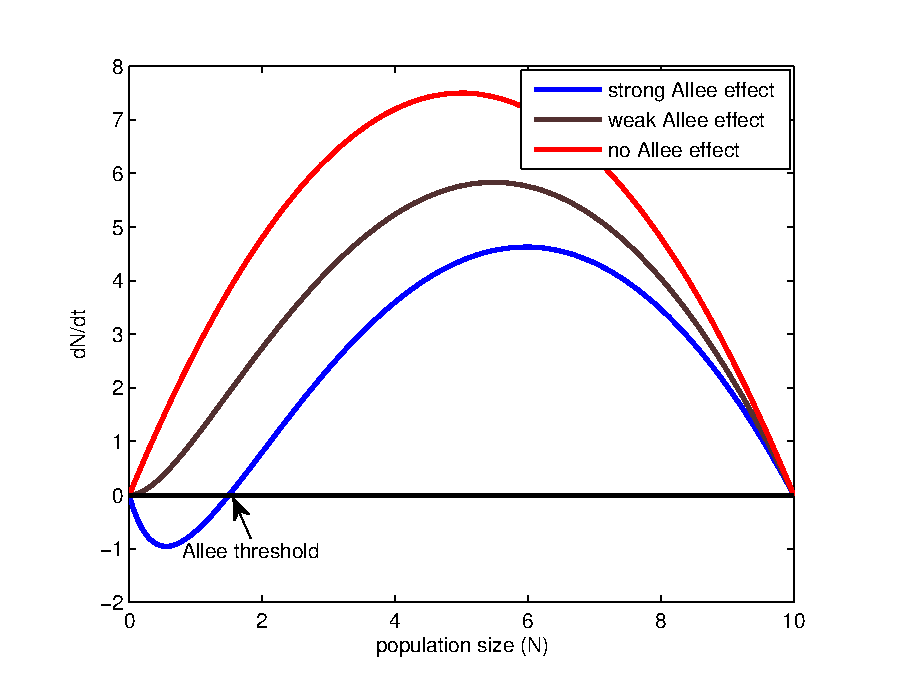
\includegraphics[width=9cm, height=6cm]{1.eps}}\]
		\begin{center} Figure 1: Plot of per capita growth rate as a function of population size.  \end{center}
	\end{figure}  
	 Allee effect is prominent in many natural species. For example, in plants, insects, marine invertebrates, in birds and mammals. In recent times, Allee effect is of great significance to ecologists. It is equally important from the theoretical aspect. Many comparisons have been done in prey-predator system with and without Allee effect. Some studies have been conducted on strong Allee effect on prey-predator model $[5]$. Weak Allee effect has been well studied by few ecologists. Hopf-bifurcation analysis with Allee effect has been carried out by many reserach scientists. \par
	To the best knowledge of the authors, a detailed analysis of strong and weak Allee effect along with Beddington Deangelis functional response has not been studied. Keeping this in mind, we reconstruct the model described by Cantrell and Consner$[3]$  by incorporating strong and weak Allee effect. The rest part of this article is arranged as follows. In next section 2 we formulate the model taking different paramenters into consideration for strong and weak Allee effect. In section 3, we discuss positivity, boundedness, existence of equilibrium points and their local stability analysis for both strong and weak Allee effect models. Numerical simulation has also been carried out to illustrate the analytical findings in section 4. Finally, this report ends with conclusion and significance of theoretical results.
	
		\section{Model Formation}
	Cantrell and Cosner$[3]$ have analyzed the dynamics of following density dependent non-linear mathematical model
	\begin{equation}
	\begin{split}
	&\frac{dx}{dt}=x\Big(1-x-\frac{cy}{1+a_1x+b_1y}\Big),\\
	&\frac{dy}{dt}=y\Big(-d-ey-\frac{fx}{1+a_1x+b_1y}\Big),\\
	&x(0)=x_0~\textgreater~0,~y(0)=y_0~\textgreater~0.
	\end{split}
	\end{equation}
	In this model prey population grows logistically and predator is survived only on the prey population. They follow Beddington Deangelis functional response to hunt the prey. \par
	Now at low and sparse population, prey exhibits strong Allee effect. Let $\beta$ be the strong Allee parameter. The prey-predator dynamics incorporated strong Allee effect in prey population is governed by the following system:
	\begin{equation}
	\begin{split}
	&\frac{dx}{dt}=rx\big(1-\frac{x}{K}\big)\Big(x-\beta\Big)-\frac{\alpha xy}{(1+ax+by)},\\
	&\frac{dy}{dt}=\frac{c\alpha xy}{(1+ax+by)}-\delta_0 y-\delta_1 y^2,
	\end{split}
	\end{equation} 
	
	On the other hand, the model with weak Allee effect is based on probability of successful mating of prey population. It is incorporated into the population growth model by multiplying the probability $AL(P)$ with birth term of prey population, where $AL(P)$ is the probability of successful mating for a female prey during the reproductive period and should follows the bellow criteria:
	\begin{enumerate}
		\item No mating occurs at zero population size, $AL(0)$=0.
		\item $AL'(P)>0$ i.e. if population size increases the probability of successful mating increases.
		\item Mating is guaranteed when the population is sufficiently large, that is $AL(P)\rightarrow 1$ as $P \rightarrow \infty.$ 
	\end{enumerate}  
	We consider the probability function as $AL(P)=\frac{x}{\theta+x},~\theta>0$ (rectangular hyperbolic). Thus the model (1) with weak Allee effect can be given as:
	\begin{equation}
	\begin{split}
	&\frac{dx}{dt}=rx\big(1-\frac{x}{K}\big)\Big(\frac{x}{\theta+x}\Big)-\frac{\alpha xy}{(1+ax+by)},\\
	&\frac{dy}{dt}=\frac{c\alpha xy}{(1+ax+by)}-\delta_0 y-\delta_1 y^2,
	\end{split}
	\end{equation}
	The biological meaning of all parameters and variables in above model is provided in Table (1).\\
	\[	\begin{tabular}{ | p{3.5cm} | p{9cm} | }
	\hline
	Variables/ Parameters& Biological meaning\\
	\hline
	~~~~~~~~~~~~x& Density of prey\\
	~~~~~~~~~~~~y& Density of predator\\
	~~~~~~~~~~~~r&Intrinsic growth rate of prey \\
	~~~~~~~~~~~~K&Carrying capacity\\
	~~~~~~~~~~~~$\theta$& Weak Allee parameter\\
	~~~~~~~~~~~~$\beta$& Strong Allee parameter\\
	~~~~~~~~~~~~$\alpha$& Attack rate of predator on prey\\
	~~~~~~~~~~~~$a$&Handling time\\
	~~~~~~~~~~~~$b$&Magnitude of interference among predators\\
	~~~~~~~~~~~~$c$& Conversion efficiency of $y$ on $x$\\
	~~~~~~~~~~~~$\delta_0$ & Natural death rate of predator\\
	~~~~~~~~~~~~$\delta_1$& Coefficient of intraspecific interference among predators\\
	\hline	
	\end{tabular}\]
	\begin{center}Table 1: Variables and parameters used in model (2) and (3).\end{center}
	\section{Dynamics of of the Model}
	In this section, we will study the dynamics of the model (2) and model (3). We will prove that the solutions of both model systems are positive as well as bounded. Then we will predict about local stability of system at each feasible  equilibrium point. First we investigate the dynamics of model system (2) having strong Allee effect in prey population.
	\subsection{Positivity and boundedness of the solution}
	It is very necessary to prove that the model is biologically well behaved before the detailed study. Positivity of solution shows that the all species survive and boundedness represents as a natural restrictions to growth as a consequence of limited resources, so it is necessary to show positivity and boundedness.\\
	From model system (2), we can write
	\[x(t)=x(0)e^{\big[\int_{0}^{t}\big\{r\big(1-\frac{x(s)}{K}\big)\big(x(s)-\beta)\big)-\frac{\alpha y(s)}{(1+ax(s)+by(s))}\big\}ds\big]},\]
	\[y(t)=y(0)e^{\big[\int_{0}^{t}\big\{\frac{c\alpha x(s)}{(1+ax(s)+by(s))}-\delta_0-\delta_1 y(s)\big\}ds\big]}\]
	which shows that all solutions remain within the first quadrant of $xy$ plane starting from an interior point.\par
	In the following lemma, we show that all solutions of system (2) are bounded which refers that the model is biologically well behaved.\\\\
	\textbf{Lemma:} \textit{The set
		\[\Omega=\Big\{(x,y): 0\leq x \leq K,~0 \leq x+\frac{1}{c}y\leq \frac{rK}{\delta}\Big\}\]
		is a positive invariant set for all the solutions initiating in the interior of the positive quadrant, where $\delta =min\{r,\delta_0\}.$\\
		Proof:} Suppose $W(t)=x(t)+\frac{1}{c}y(t)$\\
	then we have
	\[\frac{dW}{dt}=\frac{dx}{dt}+\frac{1}{c}\frac{dy}{dt} = rx\big(1-\frac{x}{K}\big)(x-\beta)-\frac{\delta_0}{c}y-\frac{\delta_1}{c}y^2 \leq \frac{4r(\beta+K)^3}{27K}-\delta W,\]
	where $\delta =min\{r\beta,\delta_0\}.$\\
	Hence it follows that
	\[\limsup_{t\rightarrow{\infty}} W(t) \leq \frac{4r (\beta+K)^3}{27K\delta}.\]
	This proves the Lemma.
	\subsubsection{Existence of equilibrium points}
	The system (1) has following equilibrium points:
	\begin{enumerate}
		\item The trivial equilibrium point $E_0(0,0).$
		\item The axial equilibrium points $E_1(\beta,0)$ and $E_2(K,0).$
		\item  The system (2) has at least one equilibrium point if the following condition holds true:
		\begin{equation}
		\beta~ \textless ~\frac{\delta_0}{c\alpha-a\delta_0}~ \textless~ K.
		\end{equation}
	\end{enumerate} 
	Proof: A positive equilibrium of system (2) is a solution of the following system of equation
	\begin{equation}
	\begin{split}
	&r(1-\frac{x}{K})(x-\beta)-\frac{\alpha y}{(1+ax+by)}=0\\
	&\frac{c\alpha x}{(1+ax+by)}-\delta_0-\delta_1 y=0.
	\end{split}
	\end{equation}
	From the first equation of system (5), when $y=0$ then $x=\beta$ or $K$ and when $x=0$ then $y=\frac{-r\beta}{\alpha+rb\beta} ~ \textless~ 0.$\\
	Checking for Derivatives,
	Eqn(2) can be written as 
	\[cx\alpha=\delta_0(1+ax+by)+\delta_1(y+axy+by^2)\]
	From above equation we get,
	\[\frac{dy}{dx}=\frac{c\alpha-\delta_0a-\delta_1ay}{\delta_0b+\delta_1+ax\delta_1+2by\delta_1}\]
	Therefore for \[\frac{dy}{dx}>0\]
	\[c\alpha>\delta_0a+\delta_1ay\]
	Now looking at Eqn(1) for checking derivatives at x=$\beta$,K.
	\[r\Big(1-\frac{x}{k})(x-\beta)=\frac{y\alpha}{1+ax+by}\] 
	\[\frac{dy}{dx}_{\lvert
	x=\beta}=\frac{r(1+\alpha\beta)\Big(1-\frac{\beta}{K})}{\alpha}
    ~ \textgreater~ 0.\]
    And
    \[\frac{dy}{dx}_{\lvert
    	x=K}=\frac{-r(1+aK)(k-\beta)}{k\alpha}
    ~ \textless~ 0.\]
	 Since the above equation is continuous and differentiable in $(\beta,K)$ and $y$ both are monotonic increasing at $x=\beta$ and monotonic decreasing at $x=K,$ and $y~\textgreater~0$ for all $x\in (\beta,K).$ Applying Rolle's  mean value theorem, there exists a point in $(\beta,K)$ and in first quadrant such that the slope of the function at that point is zero.\\
	 
The conclusion of the above discussion is both the equations of system have at least one positive solution if the second equation intersects $x-$ axis between $x=\beta$ and $x=K.$\\
	Hence, the system (2) has at least one positive equilibrium point if
	\[\beta~ \textless ~\frac{\delta_0}{c\alpha-a\delta_0}~ \textless~ K.\]
	\textbf{Remark:} There are many situations on positive equilibrium like it may or may not be exist (Fig. 1(a)), it could be unique (Fig. 1(b-c)) or there may be two positive equilibria also (Fig. 1(d)). The number of positive equilibrium for system (2) depend on values of parameters, which we have chosen. 	
	\begin{figure}[H]
		\minipage{0.5\textwidth}
		{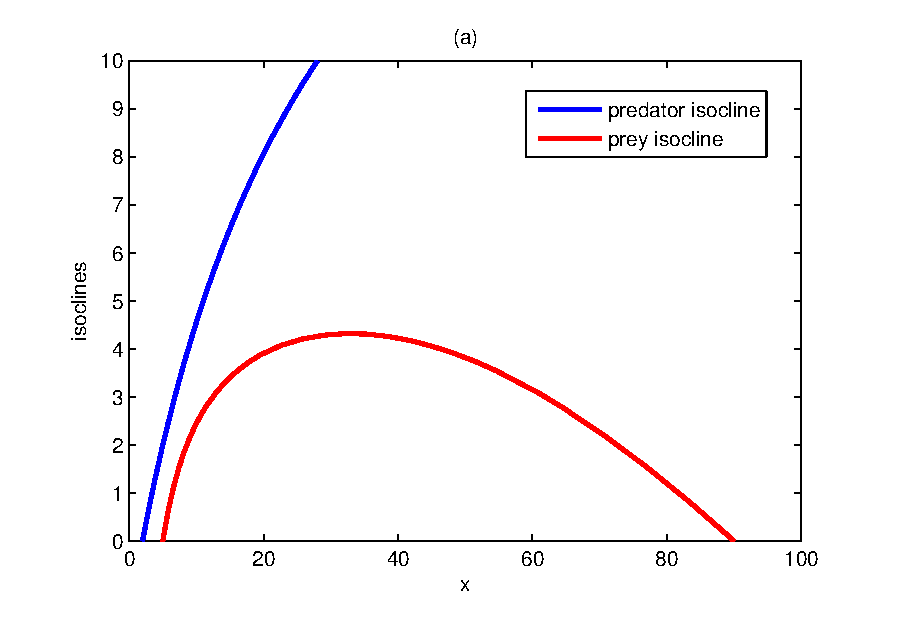
\includegraphics[scale=.6]{2.eps}}
		\endminipage\hfill
		\minipage{0.5\textwidth}
		{\includegraphics[scale=.6]{3.eps}}
		\endminipage\hfill
		\minipage{0.5\textwidth}
		{\includegraphics[scale=.6]{4.eps}}
		\endminipage\hfill
		\minipage{0.5\textwidth}
		{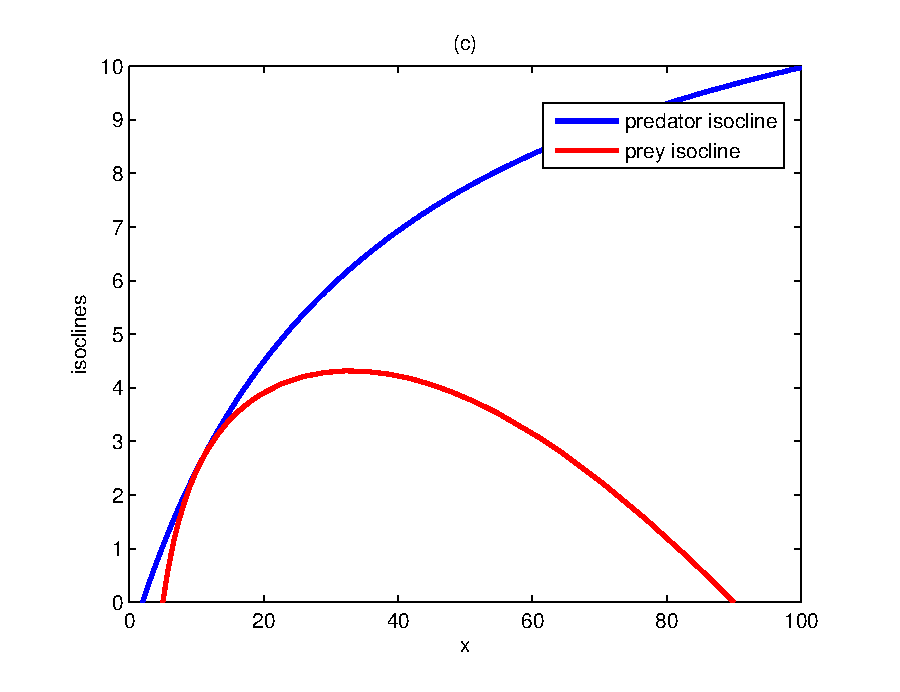
\includegraphics[scale=.6]{5.eps}}
		\endminipage\hfill
		\begin{center} Figure 1: Four possible relative of the prey and predator zero growth isoclines. (a) Interior equilibrium does not exist for the parametric values $\beta=0.6,~\delta_0=0.8~,\delta_1=0.5.$ (b-c) Interior equilibrium exists uniquely for the values of parameters $\beta=0.6,~\delta_0=4~,\delta_1=2$ and $\beta=0.6,~\delta_0=0.8~,\delta_1=1$ respectively. (d) Tow interior equilibria for parameter values $\beta=0.6,~\delta_0=0.8~,\delta_1=2.$ Rest of the parameters are same as that in (24).  \end{center}
	\end{figure}
	\subsubsection{Local stability analysis}
	To analyze the local stability behaviour of the equilibria whenever they exist, we compute the Jacobian matrix for the model system (2) and further this matrix calculated at each of equilibria. Then using Routh-Hurwitz criteria, we get following results:
	\begin{enumerate}
		\item The equilibrium Point $E_0(0,0)$ is always asymptotically stable.
		\item \begin{itemize}
			\item $E_2(\beta,0)$ is locally unstable if $c\alpha \beta~\textgreater ~\delta_0(1+a\beta).$
			\item $E_2(\beta,0)$ is saddle point having stable manifold along the $x-$axis and unstable manifold along the $y-$axis if $c\alpha \beta ~\textless~\delta_0(1+a\beta).$
		\end{itemize}
		\item \begin{itemize}
			\item $E_2(K,0)$ is locally asymptotic stable if $c\alpha K~\textless~\delta_0(1+aK).$
			\item $E_2(K,0)$ is saddle point having stable manifold along the $x-$axis and unstable manifold along the $y-$axis if $c\alpha K~\textgreater~\delta_0(1+aK).$
		\end{itemize}
	\end{enumerate}
	In order to investigate the stability behaviour of positive equilibrium, let $M(E^*)$ denotes the variational matrix evaluated at $E^*$ 
	\[M(E^*)=\begin{bmatrix}
	A_{11}&A_{12}\\A_{21}&A_{22}
	\end{bmatrix},\]
	where $A_{11}=-\frac{rx^*}{K}\Big(2x^*-(k+\beta)\Big)+\frac{\alpha ax^*y^* }{(1+ax^*+by^*)^2} \,~~A_{12}=-\frac{\alpha x^*(1+ax^*)}{(1+ax^*+by^*)^2},$\\
	$A_{21}=\frac{c\alpha y^*+c\alpha by*^2}{(1+ax^*+by^*)^2},~~A_{22}=-\frac{bc\alpha x^*y^*}{(1+ax^*+by^*)^2}-\delta_1 y^*.$\\ \\
	Then the characteristic equation of $M(E^*)$ is given by
	\begin{equation}
	\lambda^2+A_1\lambda+A_2=0,
	\end{equation}
	where $A_1=-tr(M(E^*))=-(A_{11}+A_{22})$ and $A_2=det(M(E^*))=A_{11}A_{22}-A_{12}A_{21}.$\\\\
	Using the Routh-Hurwitz criteria, both the eigenvalues of $M(E^*)$ have negative real part if and only if $A_1~\textgreater~0,~A_2~\textgreater~0.$\\
	\medskip Thus we can state the following theorem.\\ 
	\textbf{Theorem:} The system (2) is locally asymptotic stable around the interior equilibrium $E^*$ if and only if $A_1~\textgreater~0,~A_2~\textgreater~0.$\\\\
	\textbf{Remark:} It can be noted that if $A_{11}~\textless~0,$ then $A_1~\textgreater~0,~A_2~\textgreater~0.$ Consequently the interior equilibrium $E^*$ is \smallskip asymptotically stable.\\
	In equation (6), if we assume $A_2~\textless~0,$ then one eigenvalue is real and positive and other eigenvalue is real and negative.\medskip Thus, the following theorem follows:\\
	\medskip \textbf{Theorem:} If $A_2~\textless~0,$ then the interior equilibrium $E^*$ is a saddle point. \\
	Now, assume that $A_1~\textless~0,$ and $A_2~\textgreater~0.$ Then both the eigenvalues are real and positive or both the eigenvalues are \smallskip complex conjugate having positive real parts. Thus we can state the following theorem.\\
	\medskip \textbf{Theorem:} If $A_1~\textless~0,$ and $A_2~\textgreater~0,$ then the interior equilibrium $E^*$ is unstable.
	\subsubsection{Bi-stability}
	In this subsection, we investigate the possibility of multistability of model system (2).
	We will see that the model may be bistable with trivial and interior equilibrium. Bi-stability is a phenomenon where the system can converge to different equilibrium in the same parametric region based on the variation of initial condition.\par 
	In stability analysis part, we have seen that $E_0$ is always stable equilibrium and interior equilibrium $E^*$ is stable if $A_{11}~\textless ~0.$ Hence, if $A_{11}~\textless ~0$ holds, then system (2) exhibits bi-stability.

	\subsection{Dynamics of weak Allee effect model}
	\textbf{Theorem*:}\textit{ All the solutions of model system (3) with initial conditions that initiate in $R_+^2$ are positive invariant and uniformly bounded.\\
		Proof:} Solutions of model system (3) which starts in $R_+^2$ are positive invariant as well as uniformly bounded. The proof is straight forward and can be omitted.\\\\
	\subsubsection{Existence of equilibrium points}
	The system (3) has following equilibrium points:
	\begin{enumerate}
		\item The trivial equilibrium point $E_0(0,0).$
		\item The axial equilibrium point $E_2(K,0).$
		\item The system (3) has a unique interior equilibrium $E_*(x_*,y_*)$ if the following condition holds:
		\[0~ \textless ~\frac{\delta_0}{c\alpha-a\delta_0}~ \textless~ K.\]
	\end{enumerate}
	\subsubsection{Local stability analysis}
	To analyze the local stability behavior of equilibrium points, we adopt same process as we done in strong Allee case and obtained following results:
	\begin{enumerate}
		\item The equilibrium point $E_0(0,0)$ is unstable proper node.
		\item The equilibrium point $E_0(K,0)$ is stable proper node.
	\end{enumerate}
	In order to analyze the stability behavior of interior equilibrium, let $M'(E_*)$ denotes the variational matrix evaluated at $E_*$ 
	\[M'(E_*)=\begin{bmatrix}
	A'_{11}&A_{12}\\A_{21}&A_{22}
	\end{bmatrix},\]
	where $A'_{11}=-\frac{rx^*}{K(\theta+x^*)}+rx^*\Big(1-\frac{x}{k}\Big)\Big(\frac{\theta}{(\theta+x)^2}\Big)+\frac{\alpha axy}{(1+ax+by)^2},$
	$A'_{12}=\frac{-x\alpha(1+ax)}{(1+ax+by)^2}.$\\ \\
	$A'_{21}=\frac{cy\alpha(1+by)}{(1+ax+by)^2}.$
	$A'_{22}=\frac{-c\alpha bx^*y^*}{(1+ax+by)^2}-\delta_1 y*.$\\ \\
	Then the characteristic equation of $M'(E_*)$ is given by
	\begin{equation}
	\lambda^2+A'_1\lambda+A'_2=0,
	\end{equation}
	where $A'_1=-tr(M'(E_*))=-(A'_{11}+A_{22})$ and $A'_2=det(M'(E_*))=A'_{11}A_{22}-A_{12}A_{21}.$\\\\
	Using the Routh-Hurwitz criteria, both the eigenvalues of $M'(E_*)$ have negative real part if and only if $A'_1~\textgreater~0,~A'_2~\textgreater~0.$\\
	\medskip Thus we can state the following theorem.\\ 
	\textbf{Theorem:} The system (3) is locally asymptotic stable around the interior equilibrium $E'_*$ if and only if $A'_1~\textgreater~0,~A'_2~\textgreater~0.$\\
	\textbf{Remark:} It can be noted that if $A'_{11}~\textless~0,$ then the interior equilibrium $E_*$ is asymptotically stable.\\\\


	\section{Numerical Simulation}
In this section, we will present numerical simulations to validate the analytical findings, obtained in previous sections using MATLAB 2015b. As this is not a case study, real data are not available for this model, so we consider some hypothetical data.

\subsubsection{Strong Allee case}
For the model (2), we consider a set of parameters as follows:
\begin{equation}
\begin{split}
& r=0.5,~K=10,~\beta=0.4,~\alpha=0.7,\\
& a=0.04,~b=0.07,~c=0.7,~\delta_0=1,~\delta_1=0.3,
\end{split}
\end{equation}
with initial conditions $x(0)=y(0)=2.$
For the above set of values of parameters condition (4) satisfied. Thus at least positive equilibrium exists. The system (2) has only one positive equilibrium point $E^*(4.4337,2.1270).$ 
\begin{figure}[H]
	\minipage{0.5\textwidth}
	{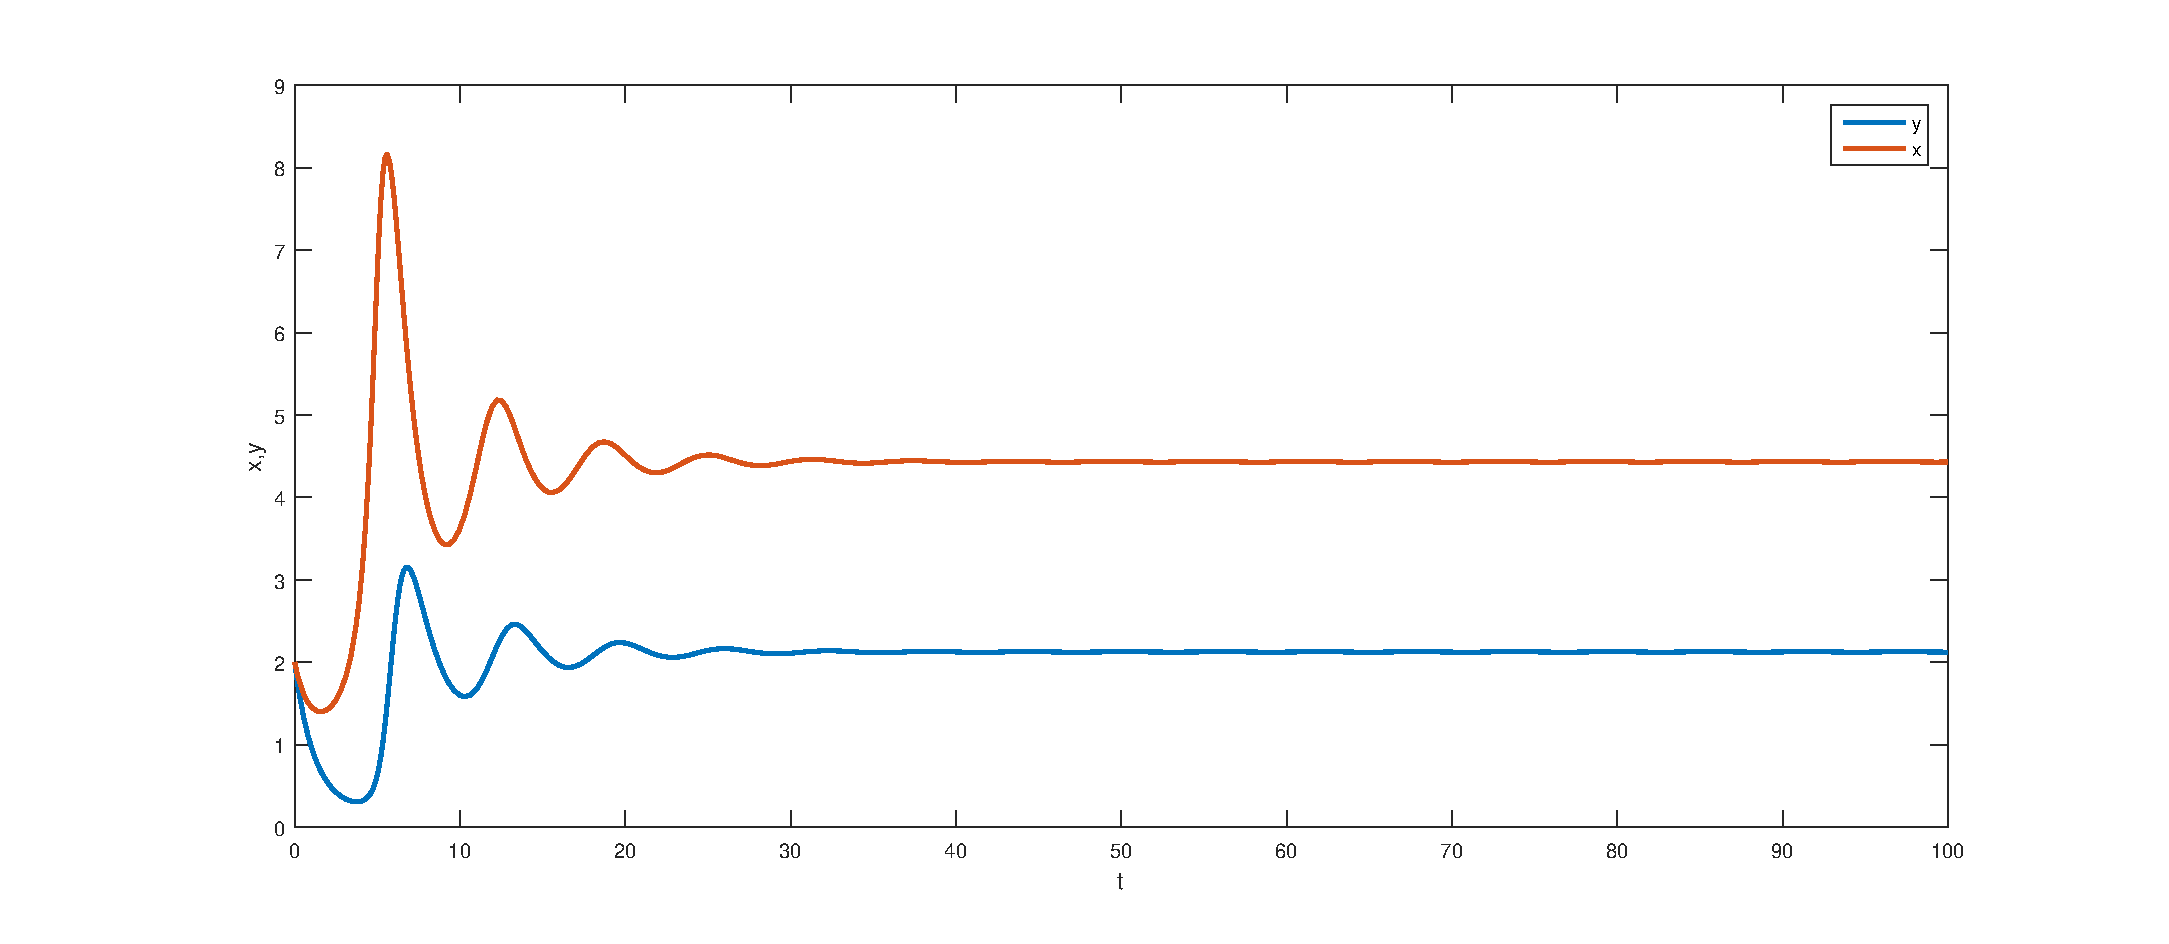
\includegraphics[width=9cm, height=6cm]{6.eps}}
	\endminipage\hfill
	\minipage{0.5\textwidth}
	{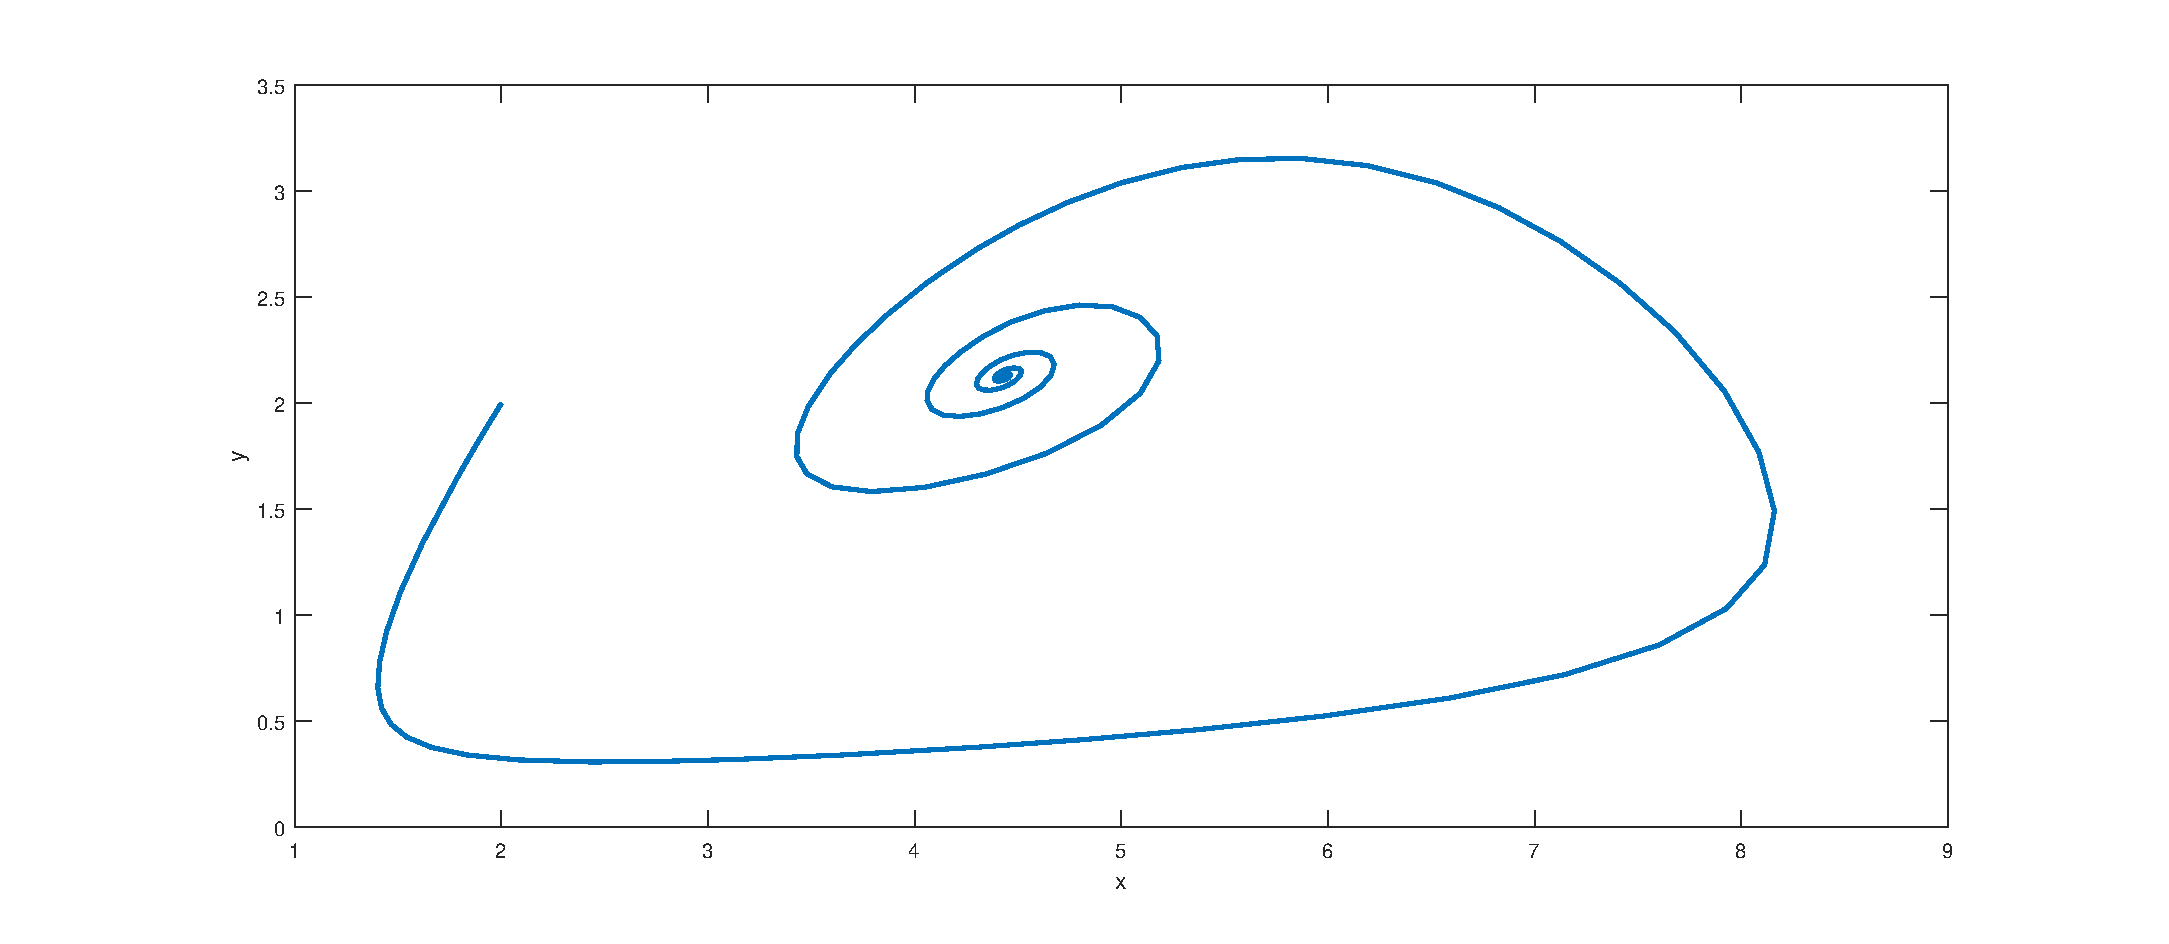
\includegraphics[width=9cm, height=6cm]{7.eps}}
	\endminipage\hfill
	\begin{center} Figure 2: (a)Time series of $x$ and $y$ and (b) phase portrait  for the set of values of parameter given in (8).  \end{center}
\end{figure}
It is also noted that $A_{11}~\textless~0$ holds for the set of parameters chosen in (8). So the interior equilibrium $E^*$ is asymptotically stable, depicted in figure 2. This figure shows that the density of prey and predator species both are decreasing initially, then some fluctuations occur and eventually settle down to the equilibrium level.
\begin{figure}[H]
	\[{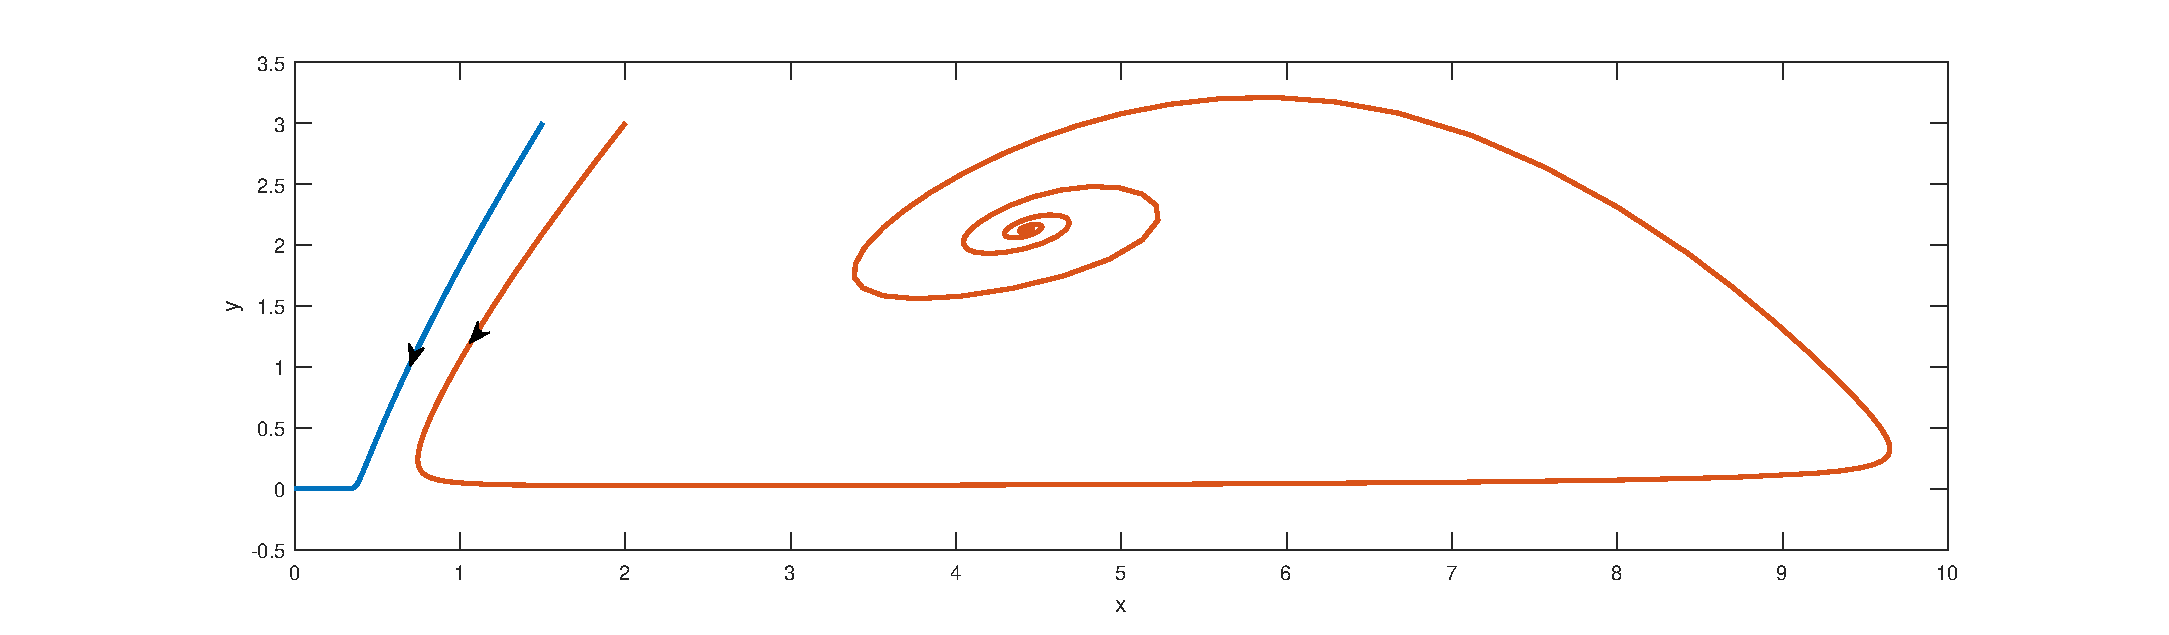
\includegraphics[width=9cm, height=6cm]{8.eps}}\]
	\begin{center} Figure 3: The system (2) exhibits bi-stability for different initial conditions and rest of the parameters have the same values as in (8).  \end{center}
\end{figure}
In figure 3, we shown the bi-stable behavior of system. For this, we plotted two trajectories of solution curves of $x$ and $y$ with different initial conditions. This figure shows that the trajectory, starts from $(1,2)$ converges to the trivial equilibrium $E_0$ and the other trajectory, initiates from $(2,2)$ converges to interior equilibrium $E^*.$
\begin{figure}[H]
	\minipage{0.5\textwidth}
	{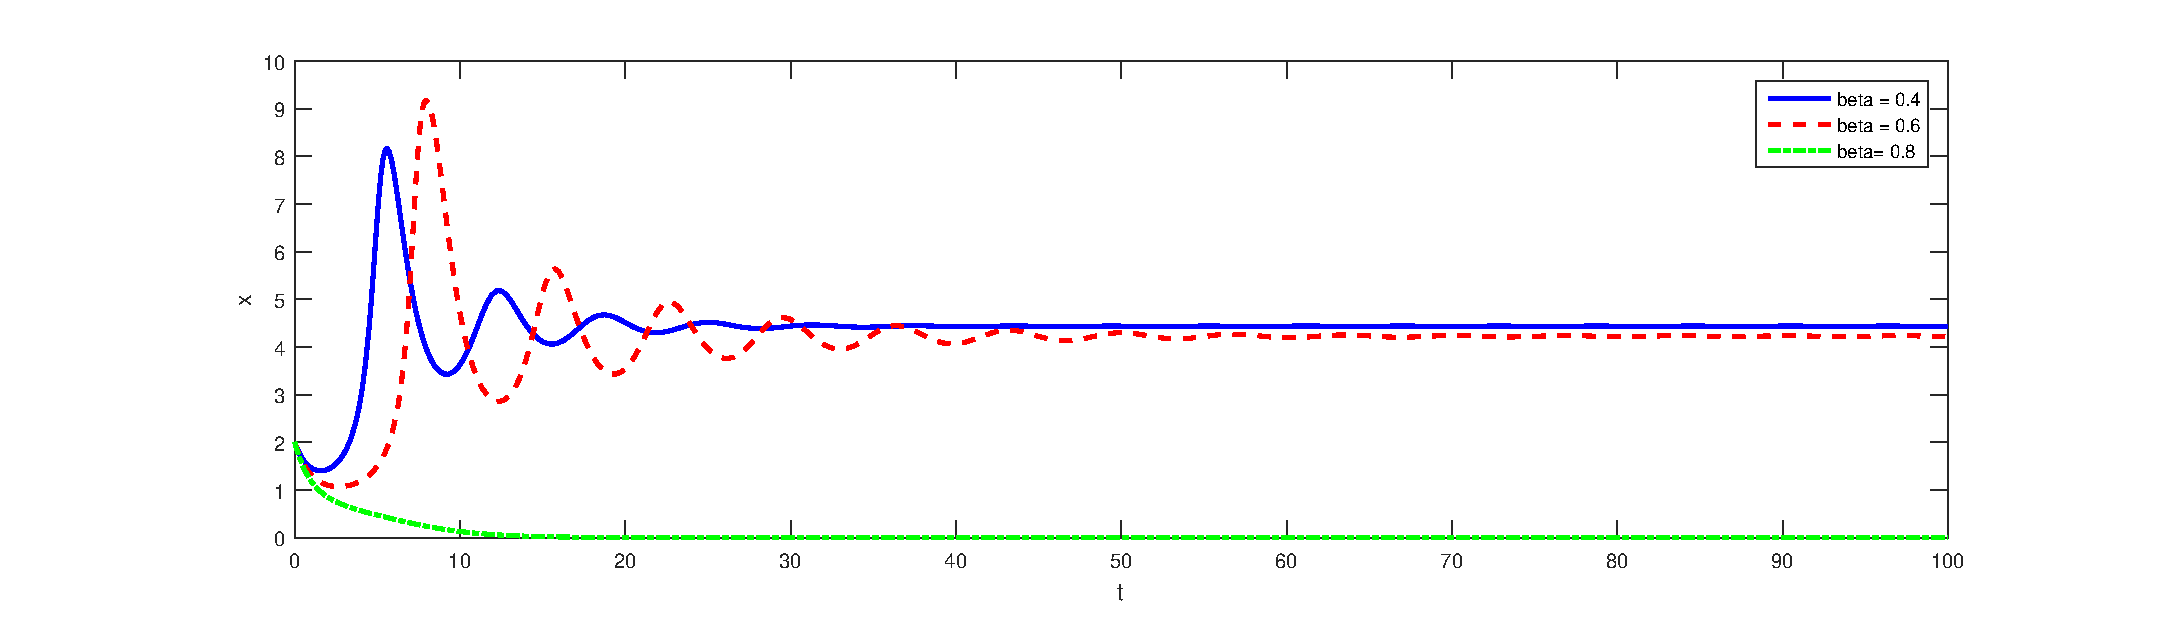
\includegraphics[width=9cm, height=6cm]{9a.eps}}
	\endminipage\hfill
	\minipage{0.5\textwidth}
	{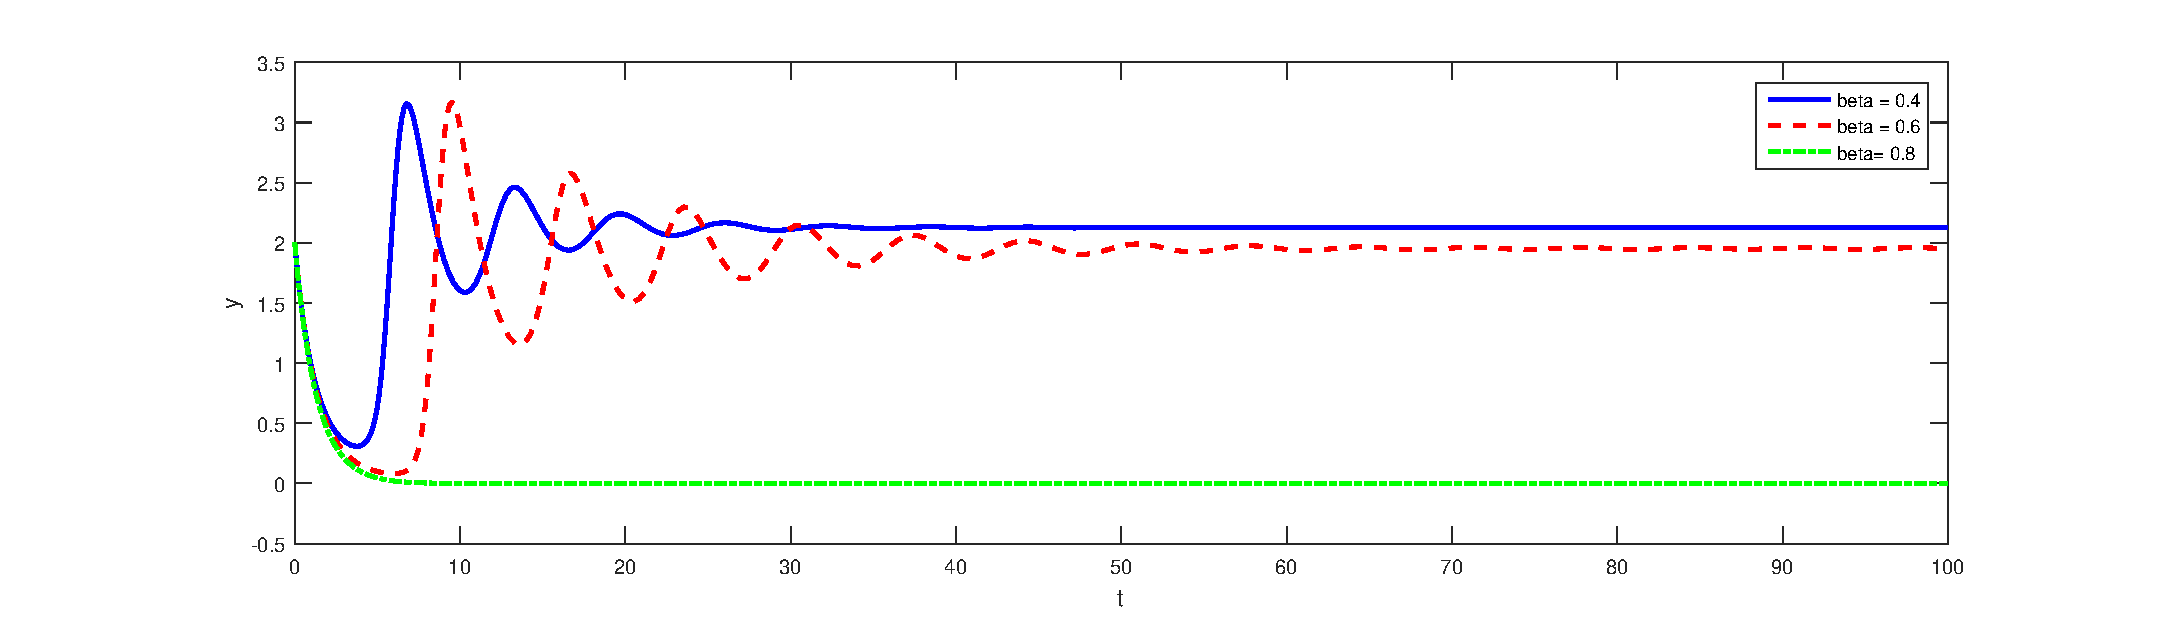
\includegraphics[width=9cm, height=6cm]{9b.eps}}
	\endminipage\hfill
	\[{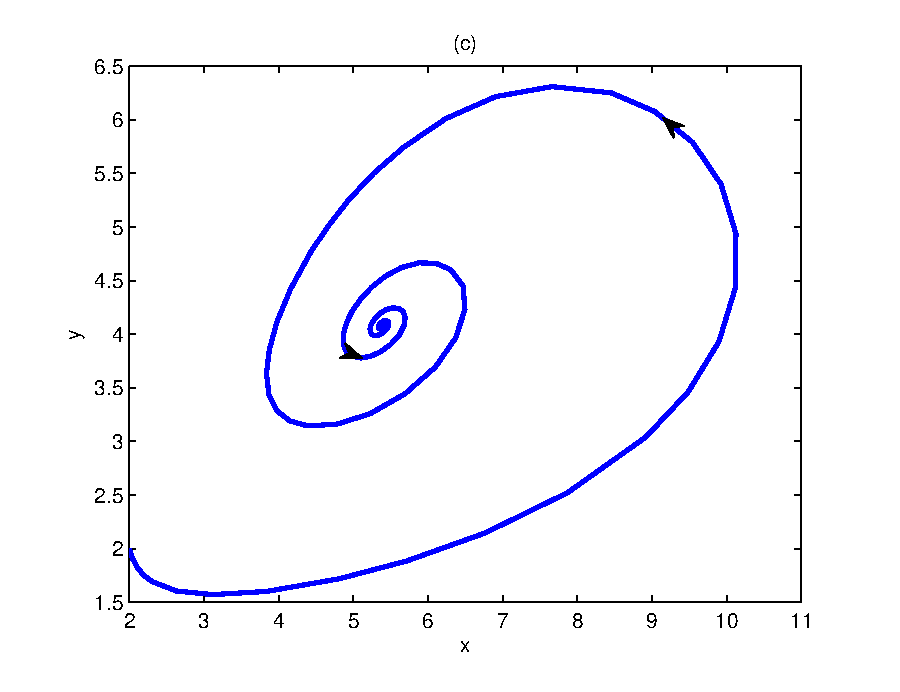
\includegraphics[width=9cm, height=6cm]{10.eps}}\]
	\begin{center} Figure 4: (a-b) Time series of $x$ and $y$ for the different values of Allee parameter $\beta$ (c) phase portrait for $\beta=0.4~\textless~\beta^*.$ $E^*$ is asymptotically stable.  \end{center}
\end{figure}
Now, we observe the dynamical behavior of the system for the variation of the Allee parameter $\beta.$ It is noted that as we increase the value of parameter $\beta,$ the time of fluctuations for both prey and predator increase. Time series analysis (4(a-b)) and phase portrait (4(c)) has shown in figure 4 for different values of $\beta,$ which refers that the system is stable for $\beta =0.4,0.6$ and for $\beta= 0.8.$ the system converges to a stable equilibrium point. At $\beta=\beta^*=0.72,$ interior equilibrium $E^*$ becomes unstable and beyond this threshold value of $\beta,$ system converges to the stable trivial equilibrium point $E_0$ for same initial conditions. Figure 5 depicts that the positive equilibrium  $E^*$ is unstable for $\beta =0.73~\textgreater~\beta^*.$\\\\
\textbf{Remark:} We can conclude after above discussion that as we increase Allee parameter $\beta,$ the life expectancy of both biological species decreases and after a critical value of $\beta~(=\beta^*)$ they move to extinction. 
\begin{figure}[H]
	\minipage{0.5\textwidth}
	{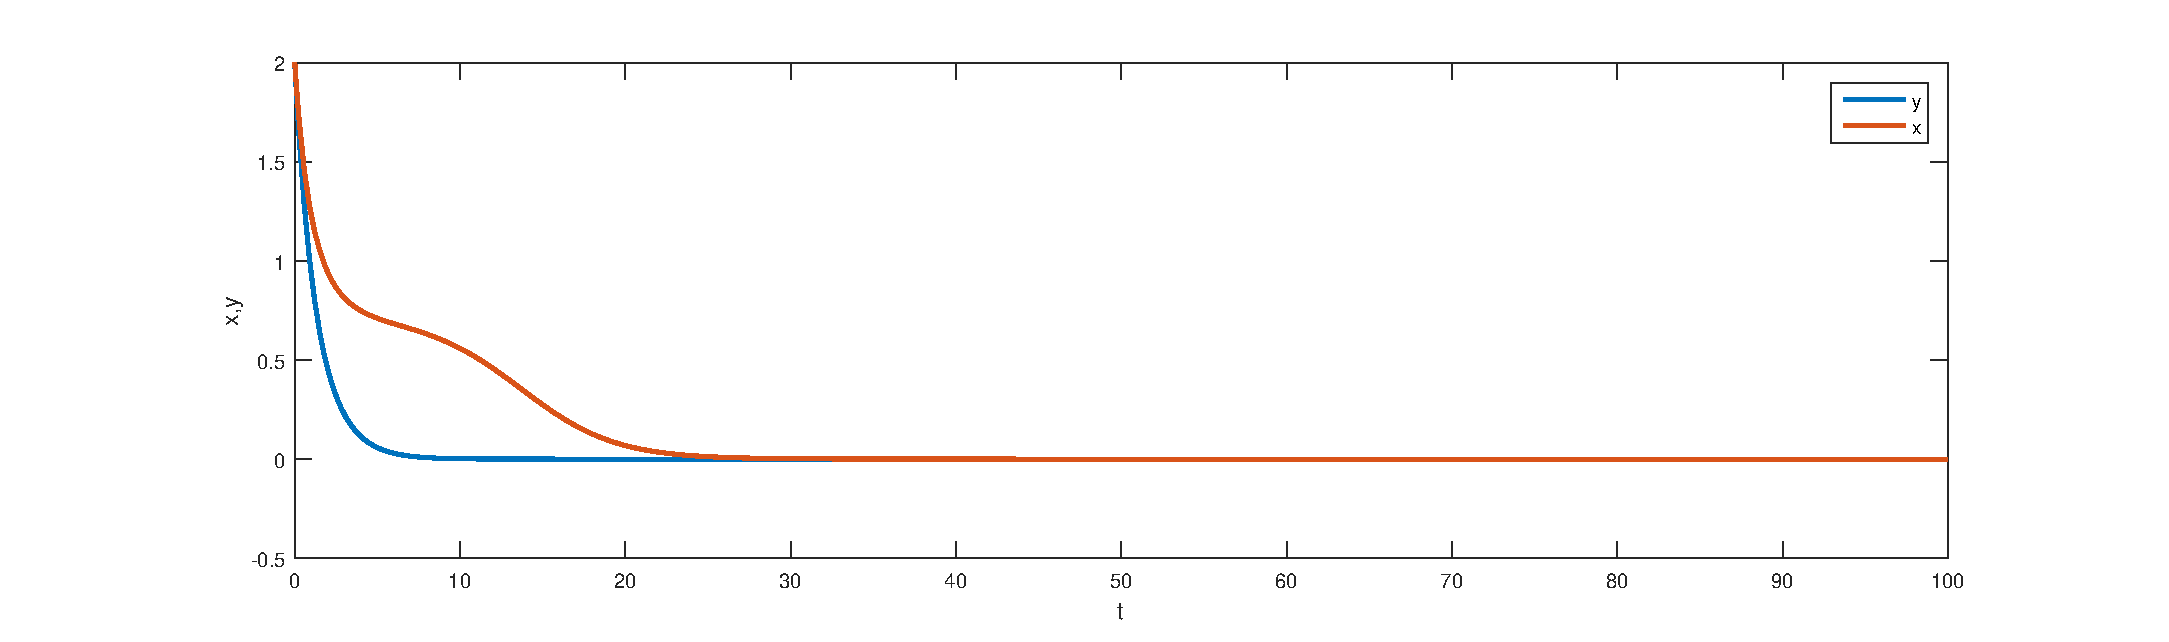
\includegraphics[width=9cm, height=6cm]{11.eps}}
	\endminipage\hfill
	\minipage{0.5\textwidth}
	{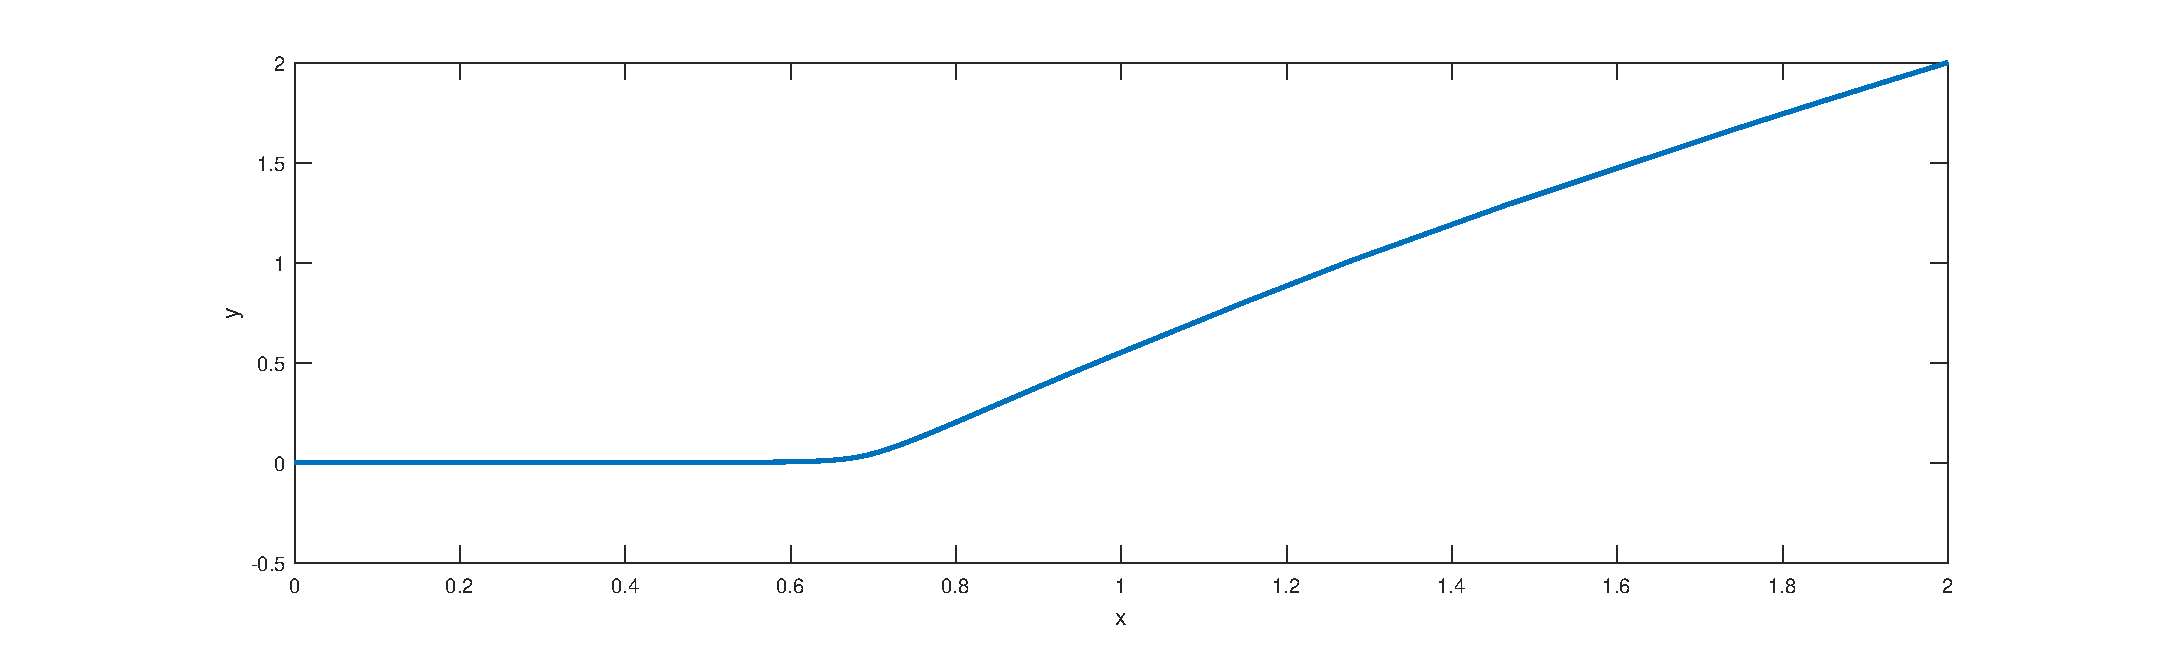
\includegraphics[width=9cm, height=6cm]{12.eps}}
	\endminipage\hfill
	\begin{center} Figure 5: Time series of $x$ and $y$ (a) and phase portrait (b) for $\beta=0.73~\textgreater~\beta^*.$ $E^*$ as the system goes to etinction and converges to $E_0(0,0).$    \end{center}
\end{figure}
In the model system (2), the parameter $a$ is also a crucial parameter because it tells us about the handling time. Therefore we will analyze how the dynamics of system changes with respect to $a$ by using Hopf-bifurcation analysis.
\begin{figure}[H]
	\minipage{0.5\textwidth}
	{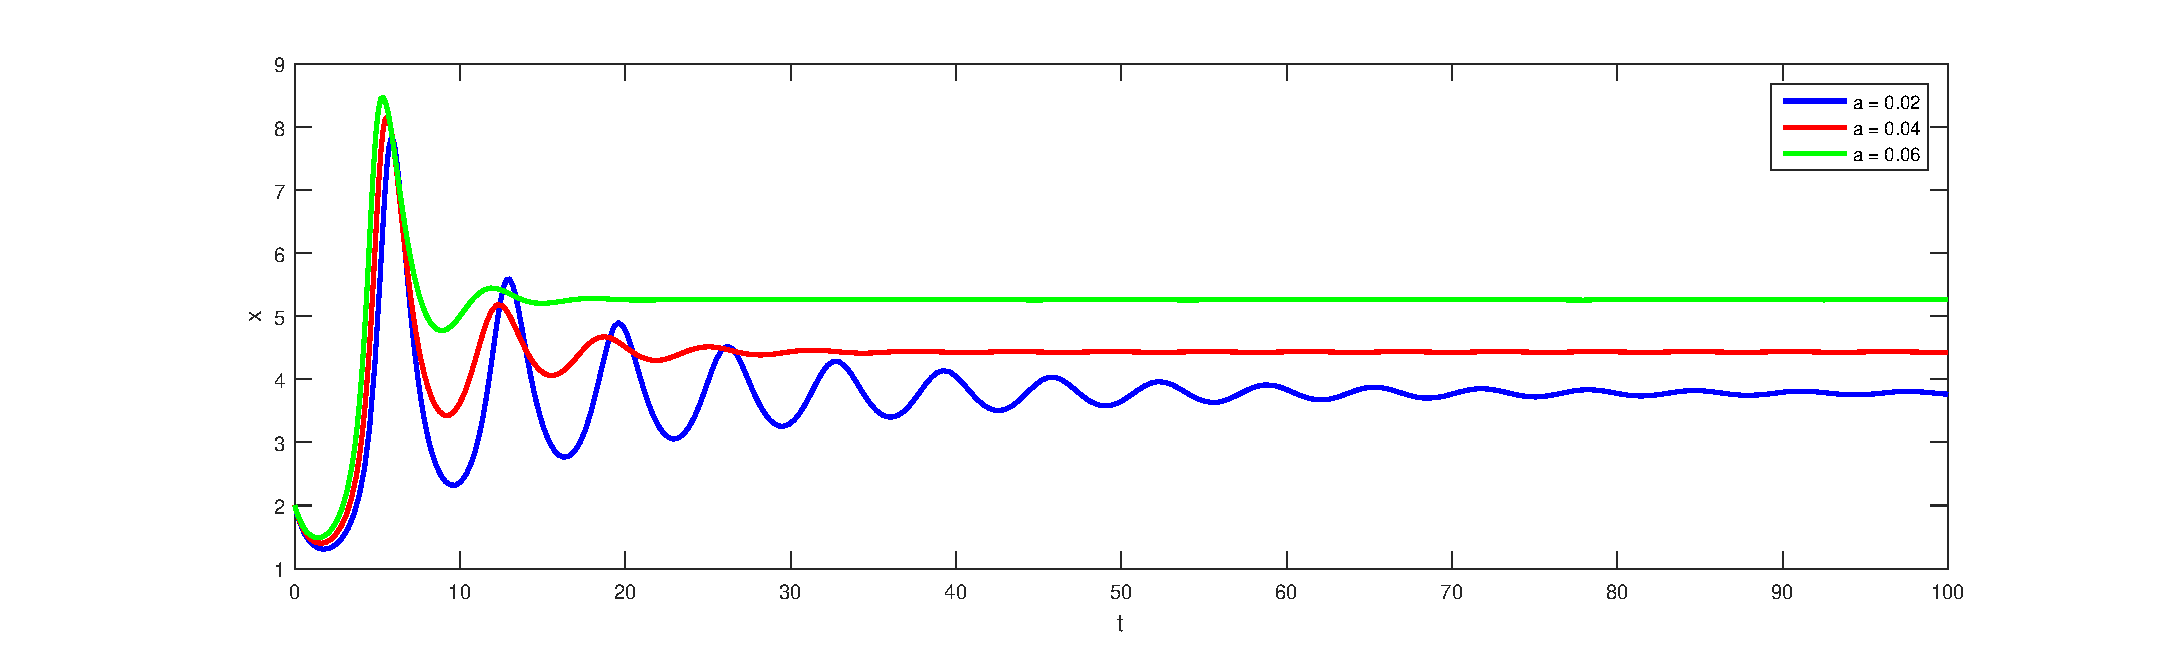
\includegraphics[width=9cm, height=6cm]{13a.eps}}
	\endminipage\hfill
	\minipage{0.5\textwidth}
	{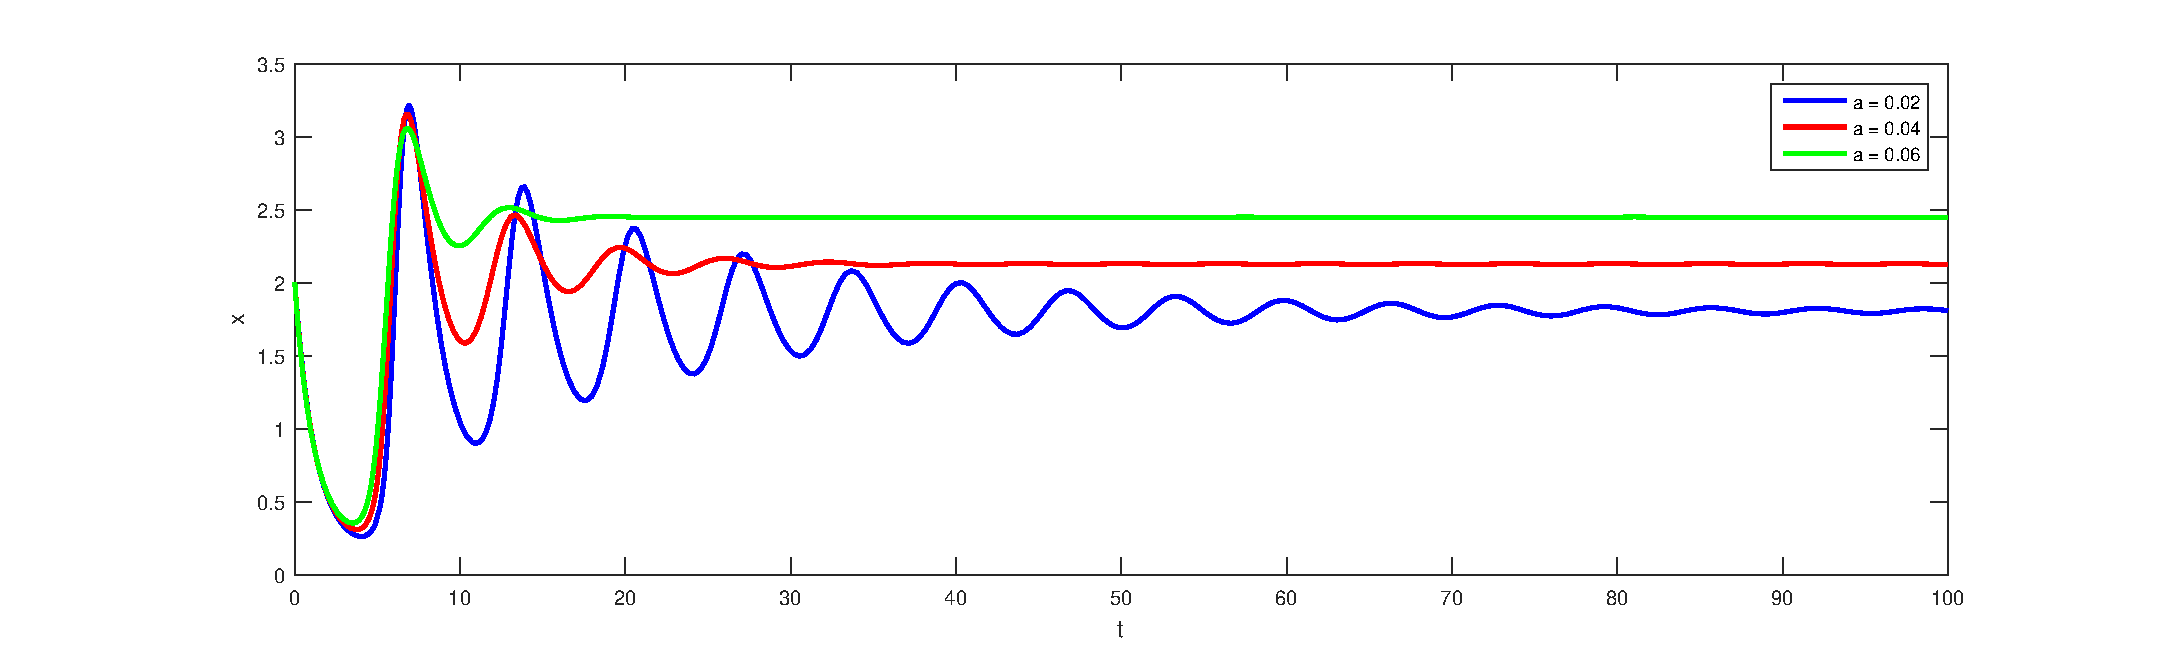
\includegraphics[width=9cm, height=6cm]{13b.eps}}
	\endminipage\hfill
	\begin{center} Figure 6: (a)Time series of $x$  (b) Time series of $y$  for different values of parameter $a$   \end{center}
\end{figure}
We observe that with the increase in handling time the system gains more stablity.
\begin{figure}[H]
	\minipage{0.5\textwidth}
	{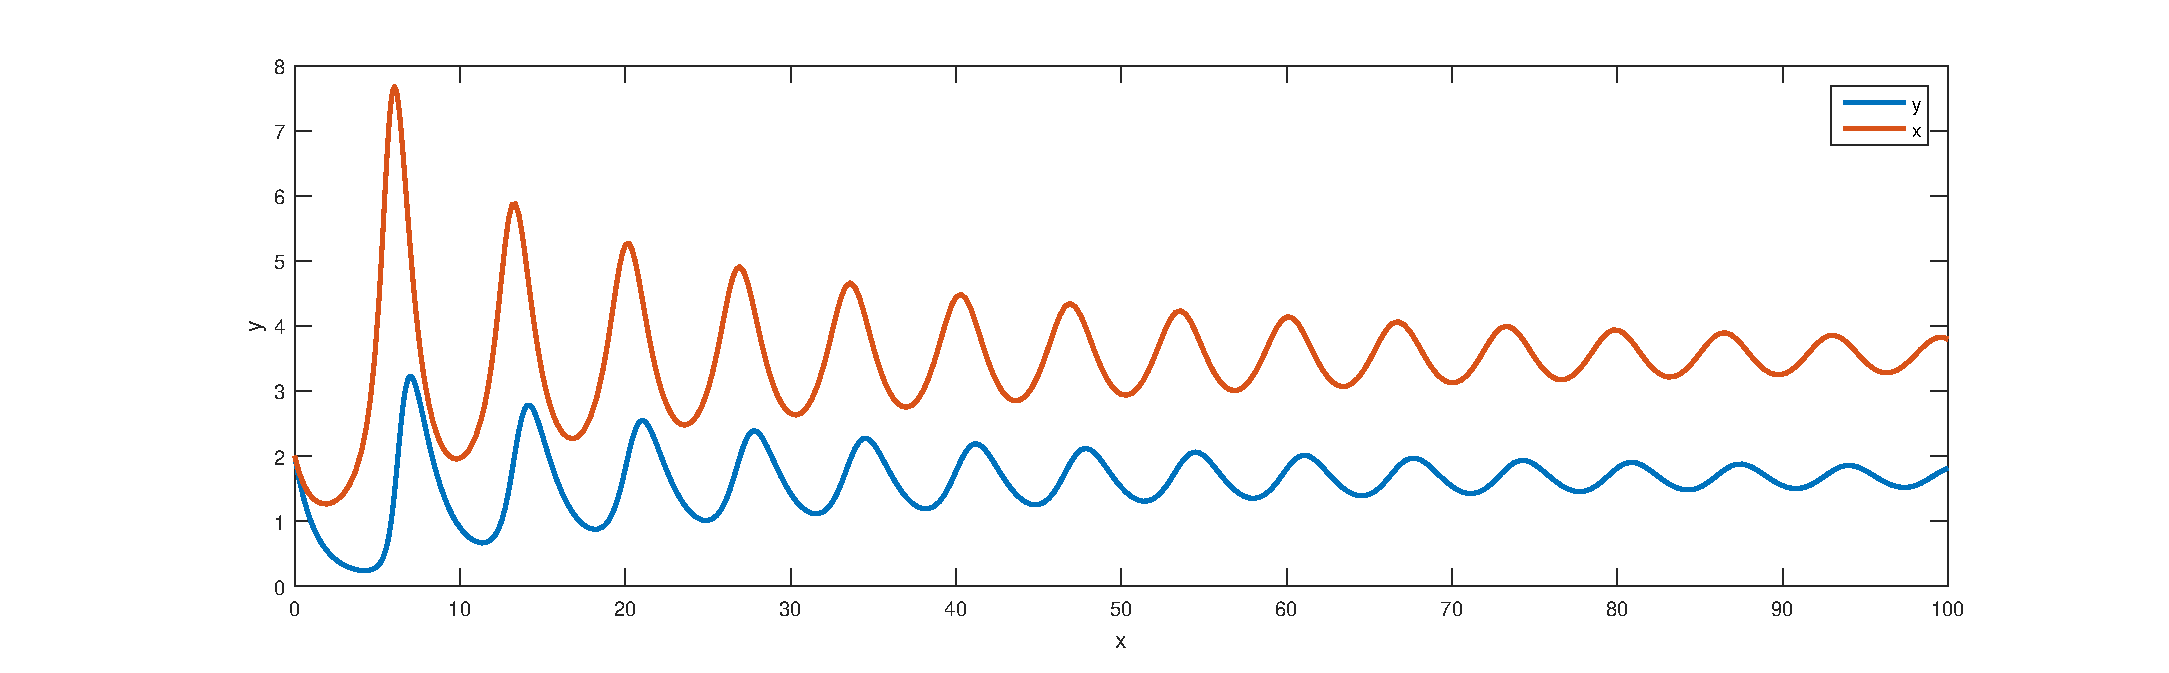
\includegraphics[width=9cm, height=6cm]{14a.eps}}
	\endminipage\hfill
	\minipage{0.5\textwidth}
	{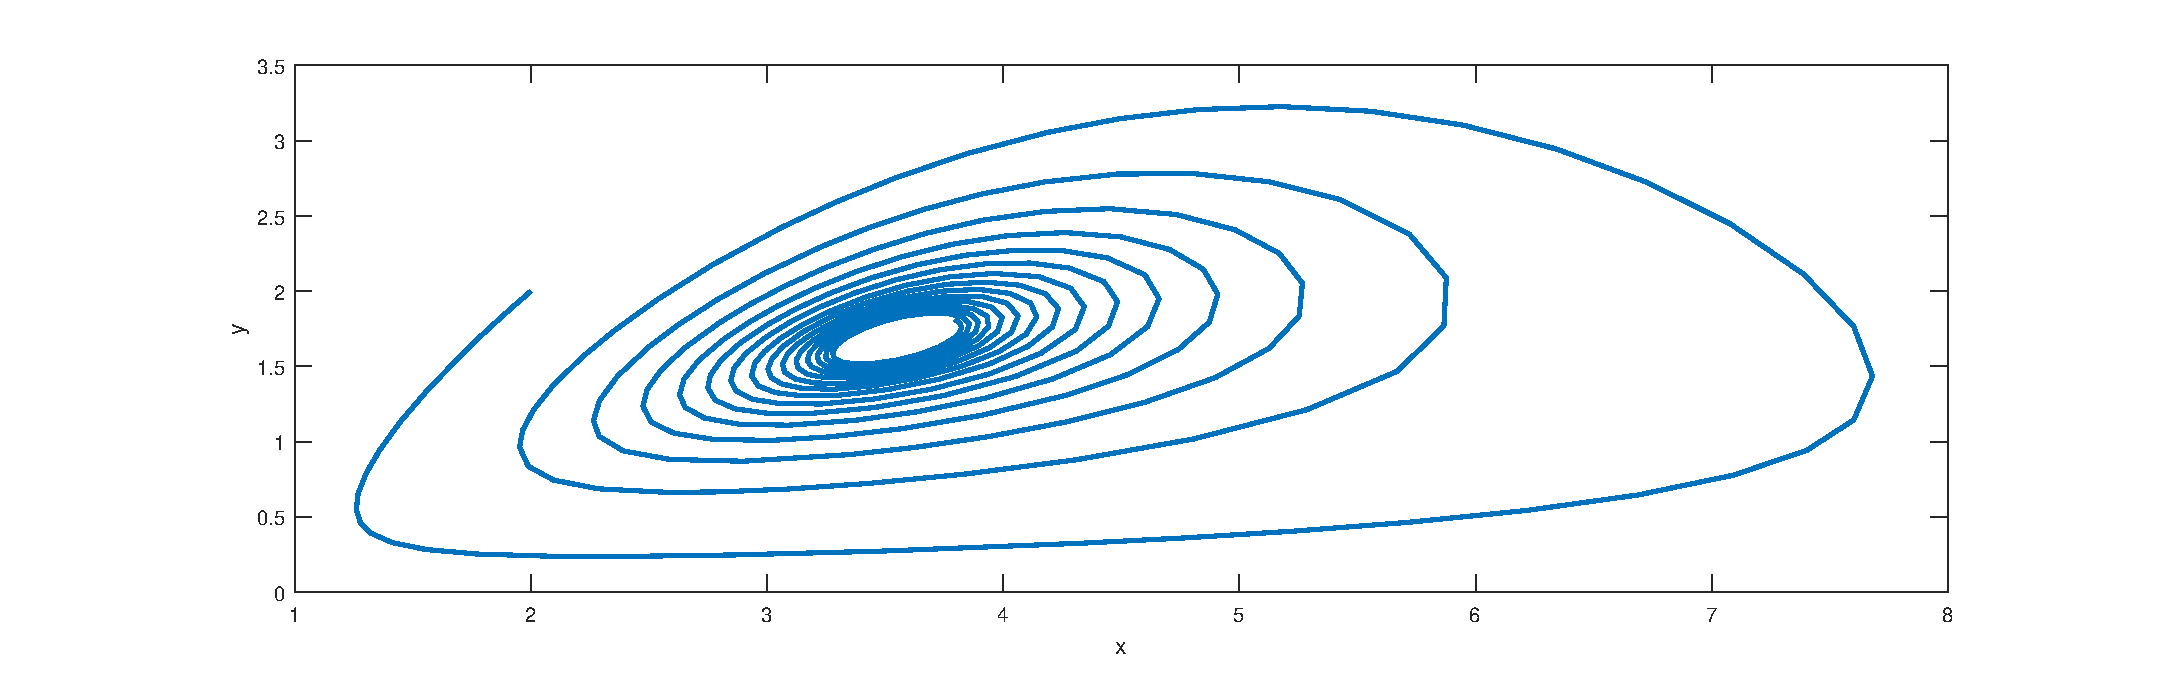
\includegraphics[width=9cm, height=6cm]{14b.eps}}
	\endminipage\hfill
	\begin{center} Figure 7: (a)Time series of $x,y$  (b)  of $y$ vs $x$ for Hopf-Bifurcation of parameter $a$  \end{center}
\end{figure}
The system (2) shows Hopf-bifurcation at $a=a^*=0.011$ and values of other parameters are same as in (8). In figure 7 we depicted time series (Fig. 7(a)) and phase portrait of the system (Fig. 7(b)) for $a=0.010~\textless~a^*=0.011,$ which refers that the system (2) has periodic solutions. 
 
In the model system (2), the parameter $b$ is of great significance because it gives us an idea about the magnitude of interference among predators. Therefore we will analyze how the dynamics of system changes with respect to $b$ by using Hopf-bifurcation analysis.
\begin{figure}[H]
	\minipage{0.5\textwidth}
	{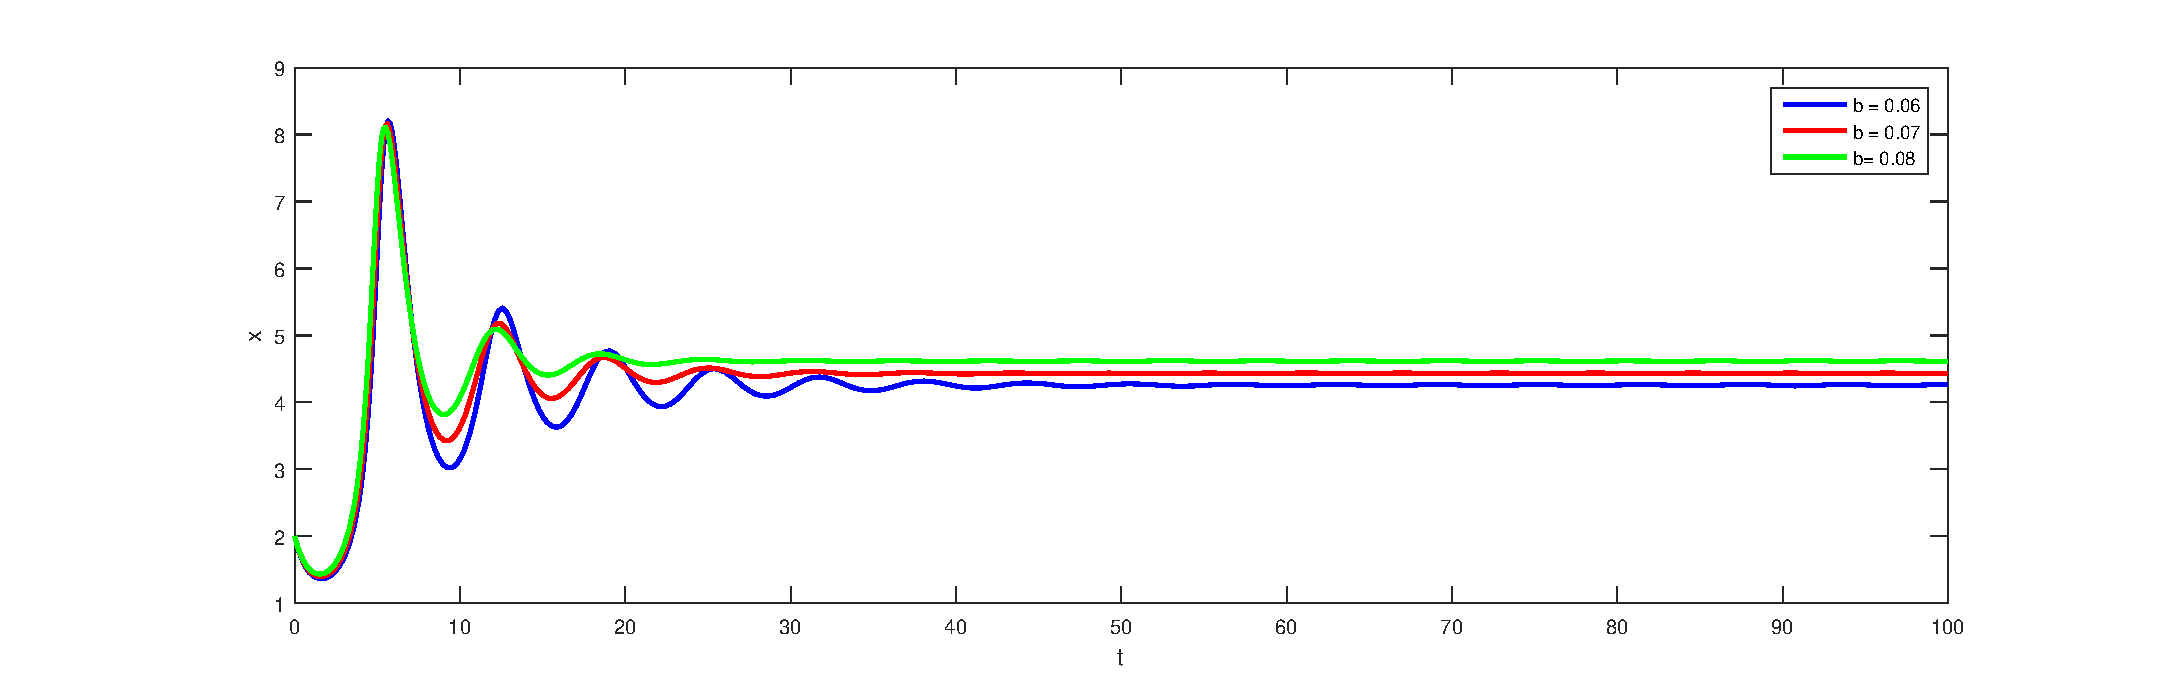
\includegraphics[width=9cm, height=6cm]{15a.eps}}
	\endminipage\hfill
	\minipage{0.5\textwidth}
	{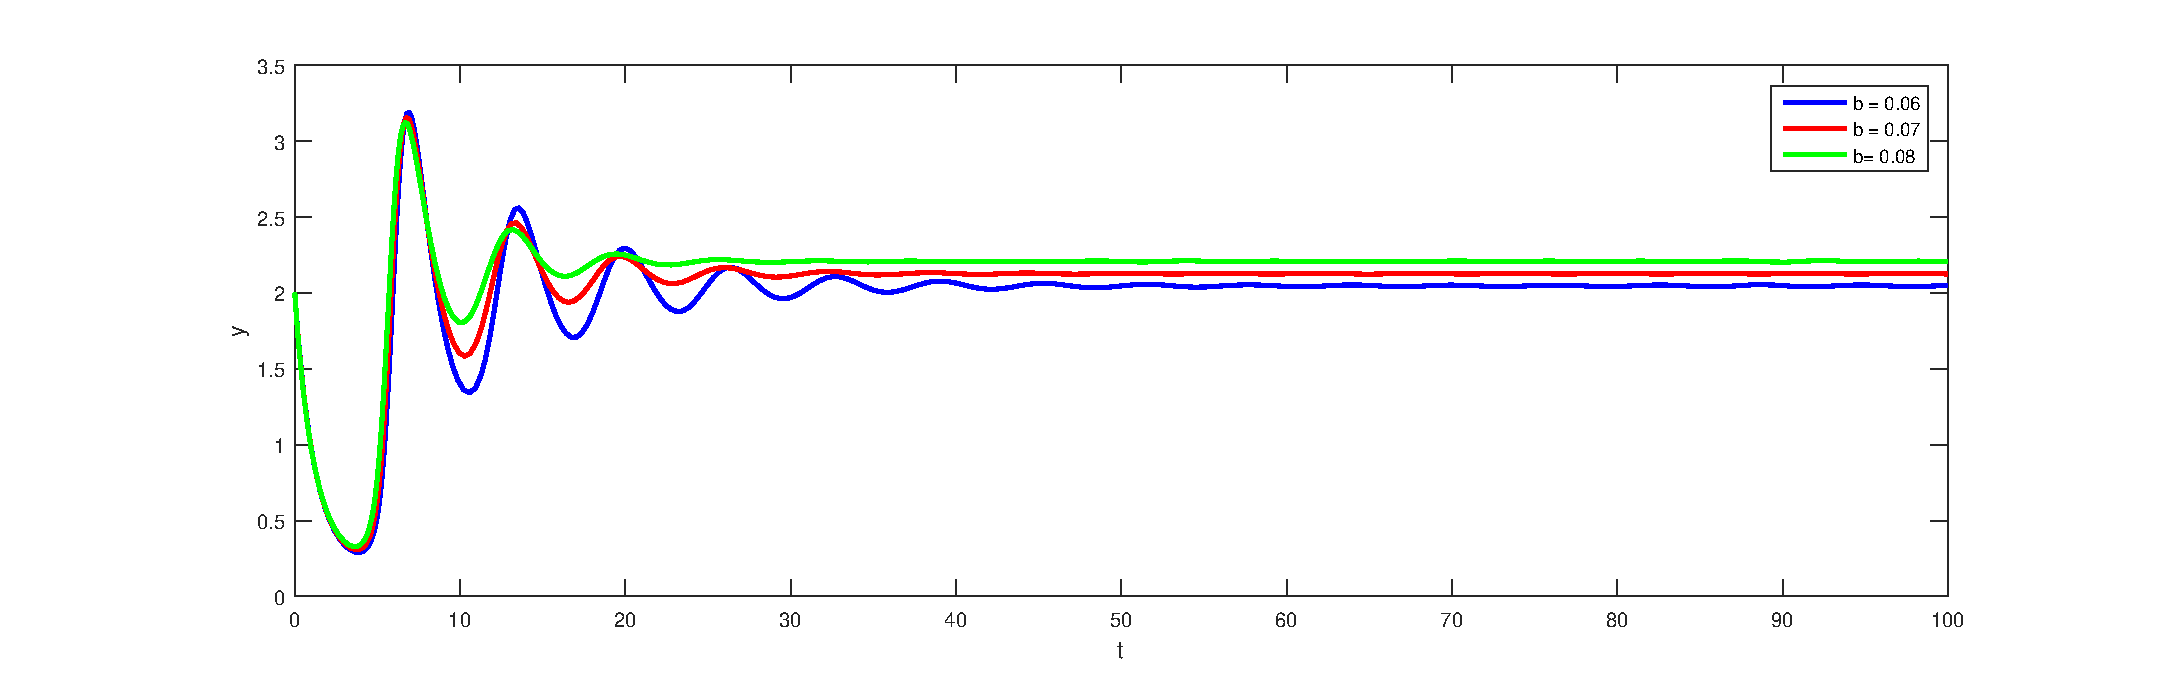
\includegraphics[width=9cm, height=6cm]{15b.eps}}
	\endminipage\hfill
	\begin{center} Figure 8: (a)Time series of $x$  (b) Time series of $y$  for different values of parameter $b$   \end{center}
\end{figure}
From figure 8, we observe that as the mutual interaction increases the system tends to become more stable.
\begin{figure}[H]
	\minipage{0.5\textwidth}
	{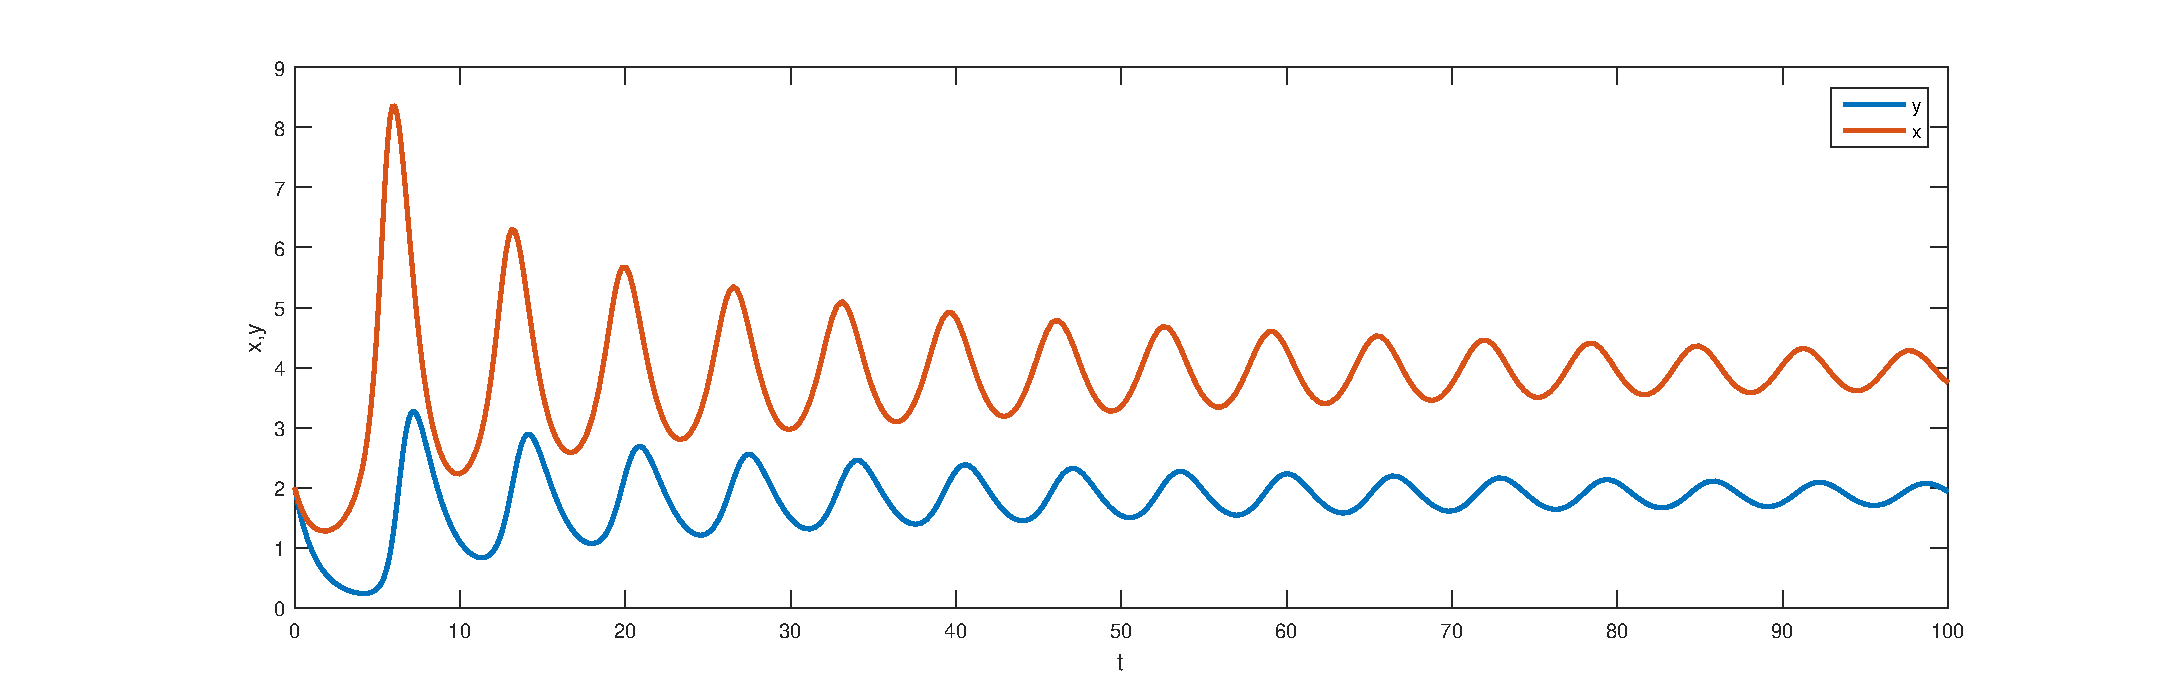
\includegraphics[width=9cm, height=6cm]{16a.eps}}
	\endminipage\hfill
	\minipage{0.5\textwidth}
	{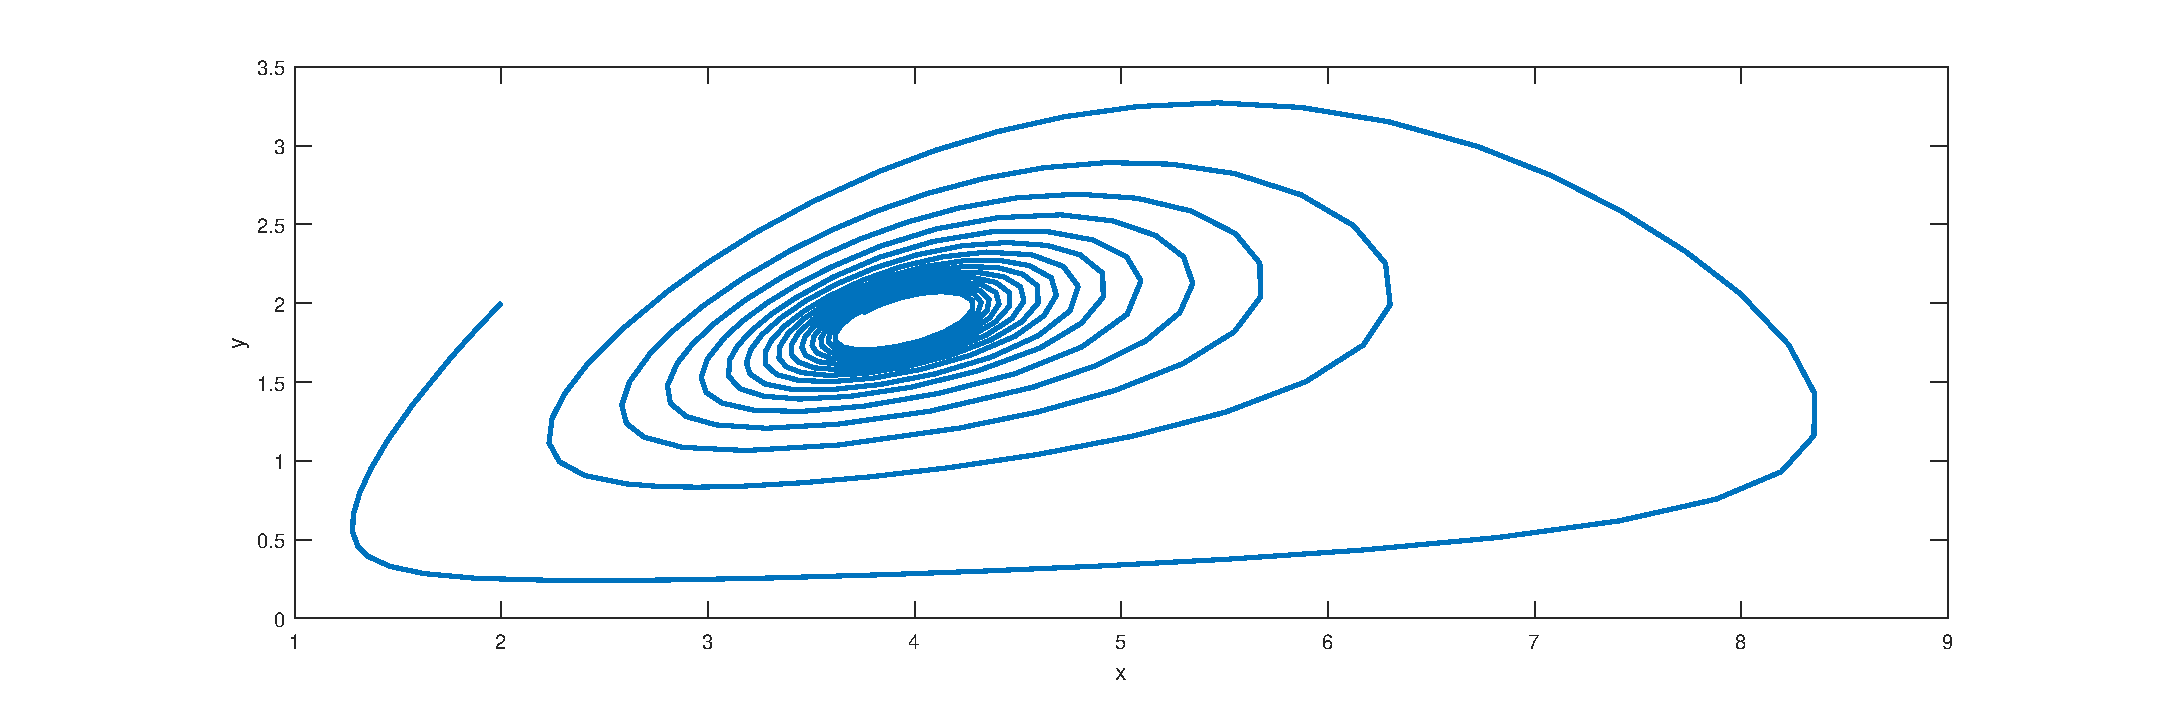
\includegraphics[width=9cm, height=6cm]{16b.eps}}
	\endminipage\hfill
	\begin{center} Figure 9: (a)Time series of $x,y$  (b)  of $y$ vs $x$ for Hopf-Bifurcation of parameter $b$   \end{center}
\end{figure}
The system (2) shows Hopf-bifurcation at $b=b^*=0.041$ and values of other parameters are same as in (8). In figure 9 we depicted time series (Fig. 9(a)) and phase portrait of the system (Fig. 9(b)) for $b=0.040~\textless~b^*=0.041,$ which refers that the system (2) is unstable.

Also in model (2), the parameter $\delta_0$ is also important because it tells us about about the natural death rate of the predators. Therefore we will analyze how the dynamics of system changes with respect to $\delta_0$ by using Hopf-bifurcation analysis.
\begin{figure}[H]
	\minipage{0.5\textwidth}
	{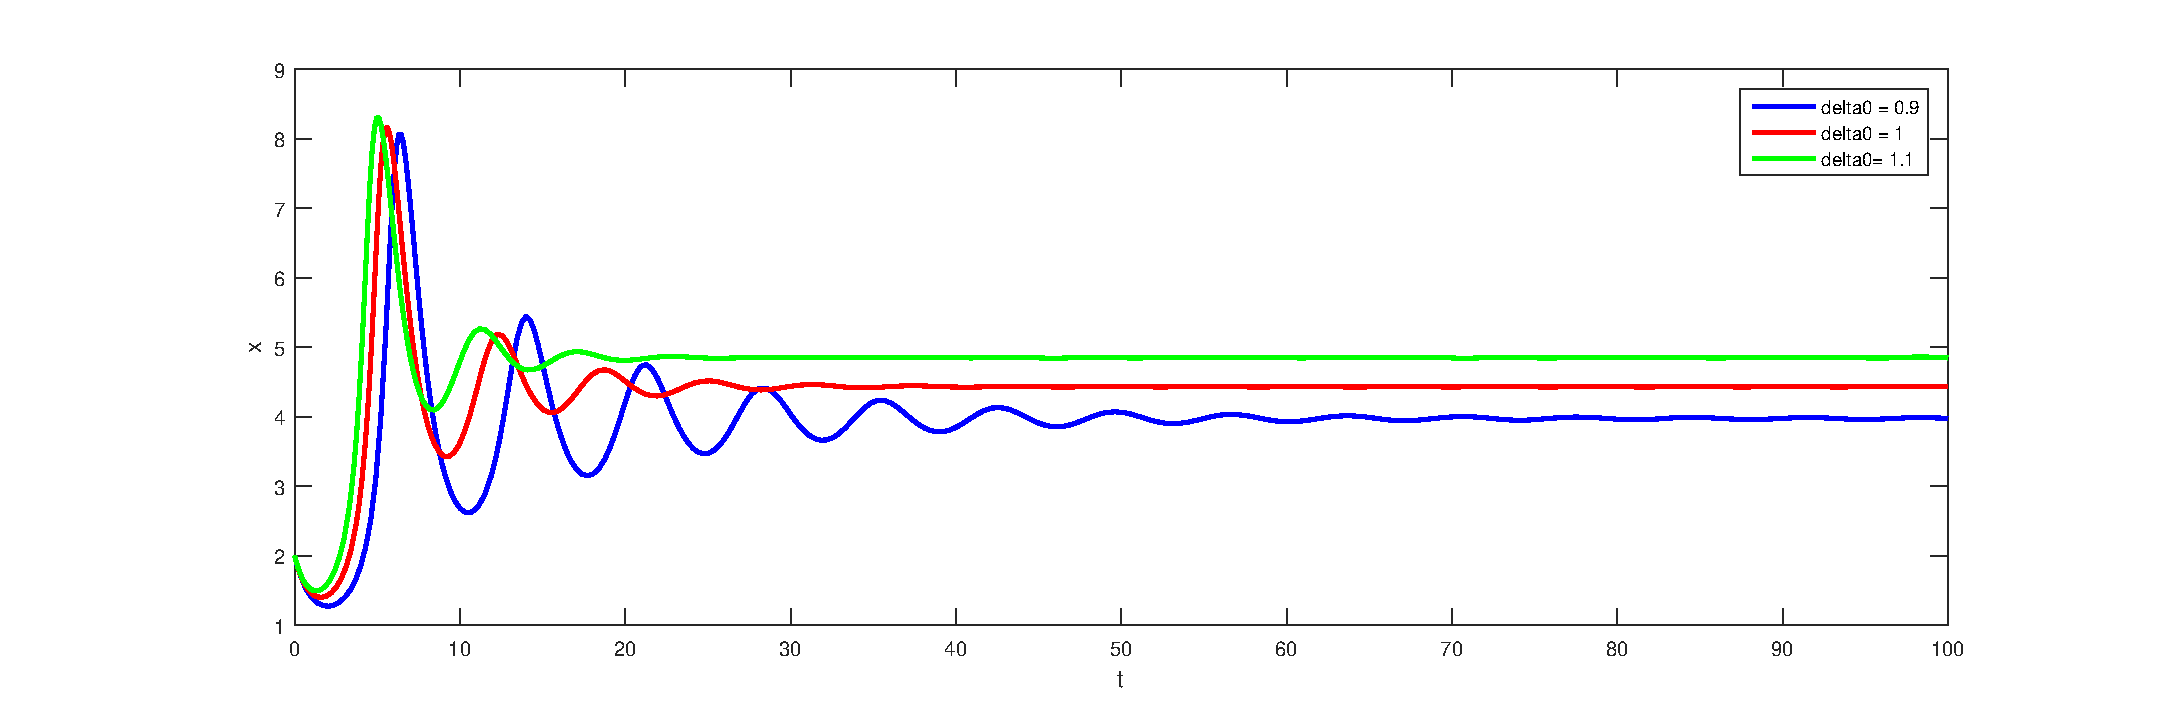
\includegraphics[width=9cm, height=6cm]{17a.eps}}
	\endminipage\hfill
	\minipage{0.5\textwidth}
	{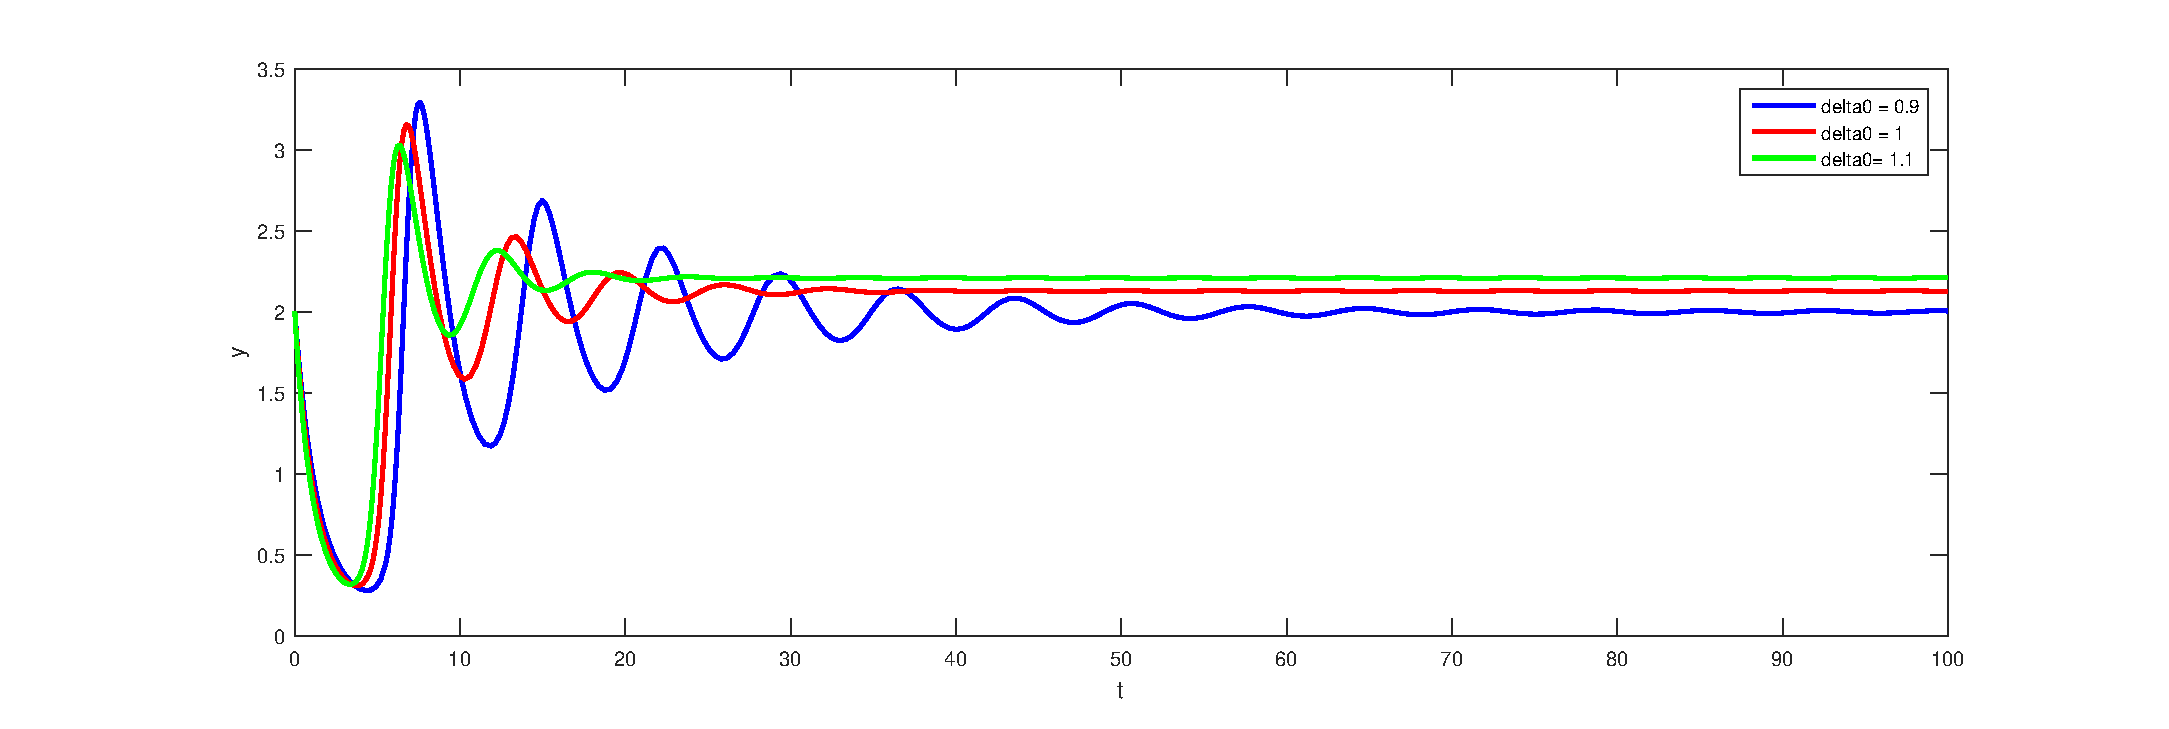
\includegraphics[width=9cm, height=6cm]{17b.eps}}
	\endminipage\hfill
	\begin{center} Figure 10: (a)Time series of $x$  (b) Time series of $y$  for different values of parameter $\delta_0$   \end{center}
\end{figure}
From figure 10, we observe that as the natural death rate of the predator increases the system tends to become more stable.
\begin{figure}[H]
	\minipage{0.5\textwidth}
	{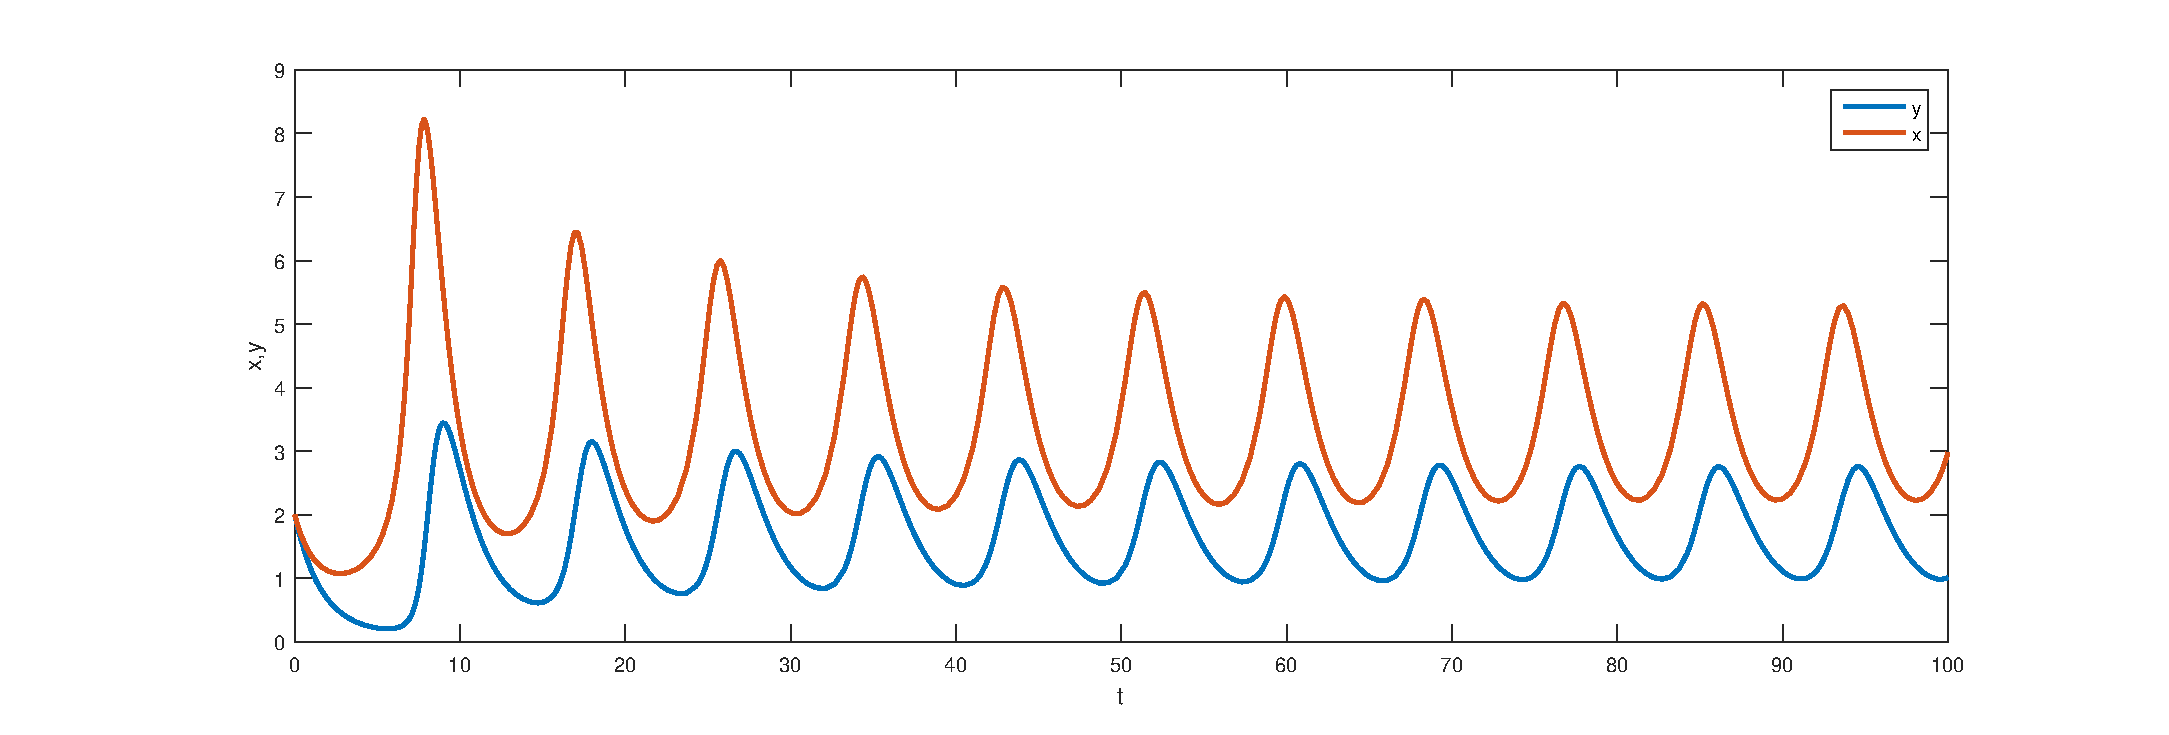
\includegraphics[width=9cm, height=6cm]{18a.eps}}
	\endminipage\hfill
	\minipage{0.5\textwidth}
	{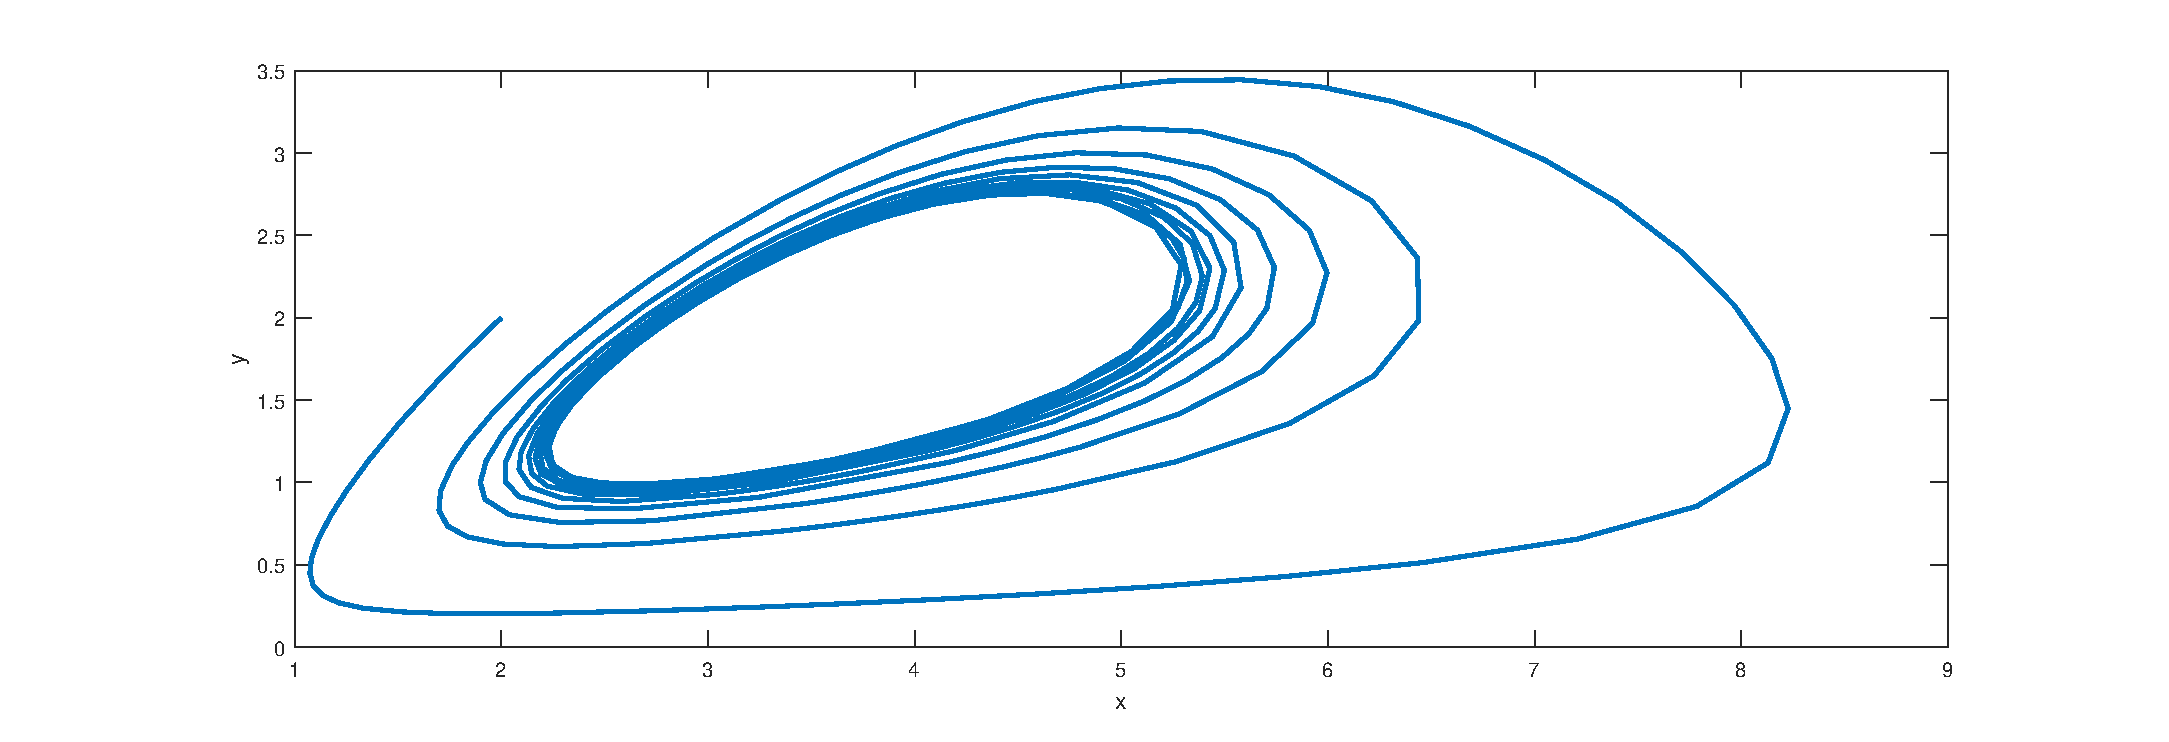
\includegraphics[width=9cm, height=6cm]{18b.eps}}
	\endminipage\hfill
	\begin{center} Figure 11: (a)Time series of $x,y$  (b)  of $y$ vs $x$ for Hopf-Bifurcation of parameter $\delta_0$   \end{center}
\end{figure}
The system (2) shows Hopf-bifurcation at $\delta_0=\delta_0^*=0.87$ and values of other parameters are same as in (8). In figure 11 we depicted time series (Fig. 7(a)) and phase portrait of the system (Fig. 7(b)) for $\delta_0=0.83~\textless~\delta_0^*=0.87,$ which refers that the system (2) has periodic solutions.
\begin{figure}[H]
	\minipage{0.5\textwidth}
	{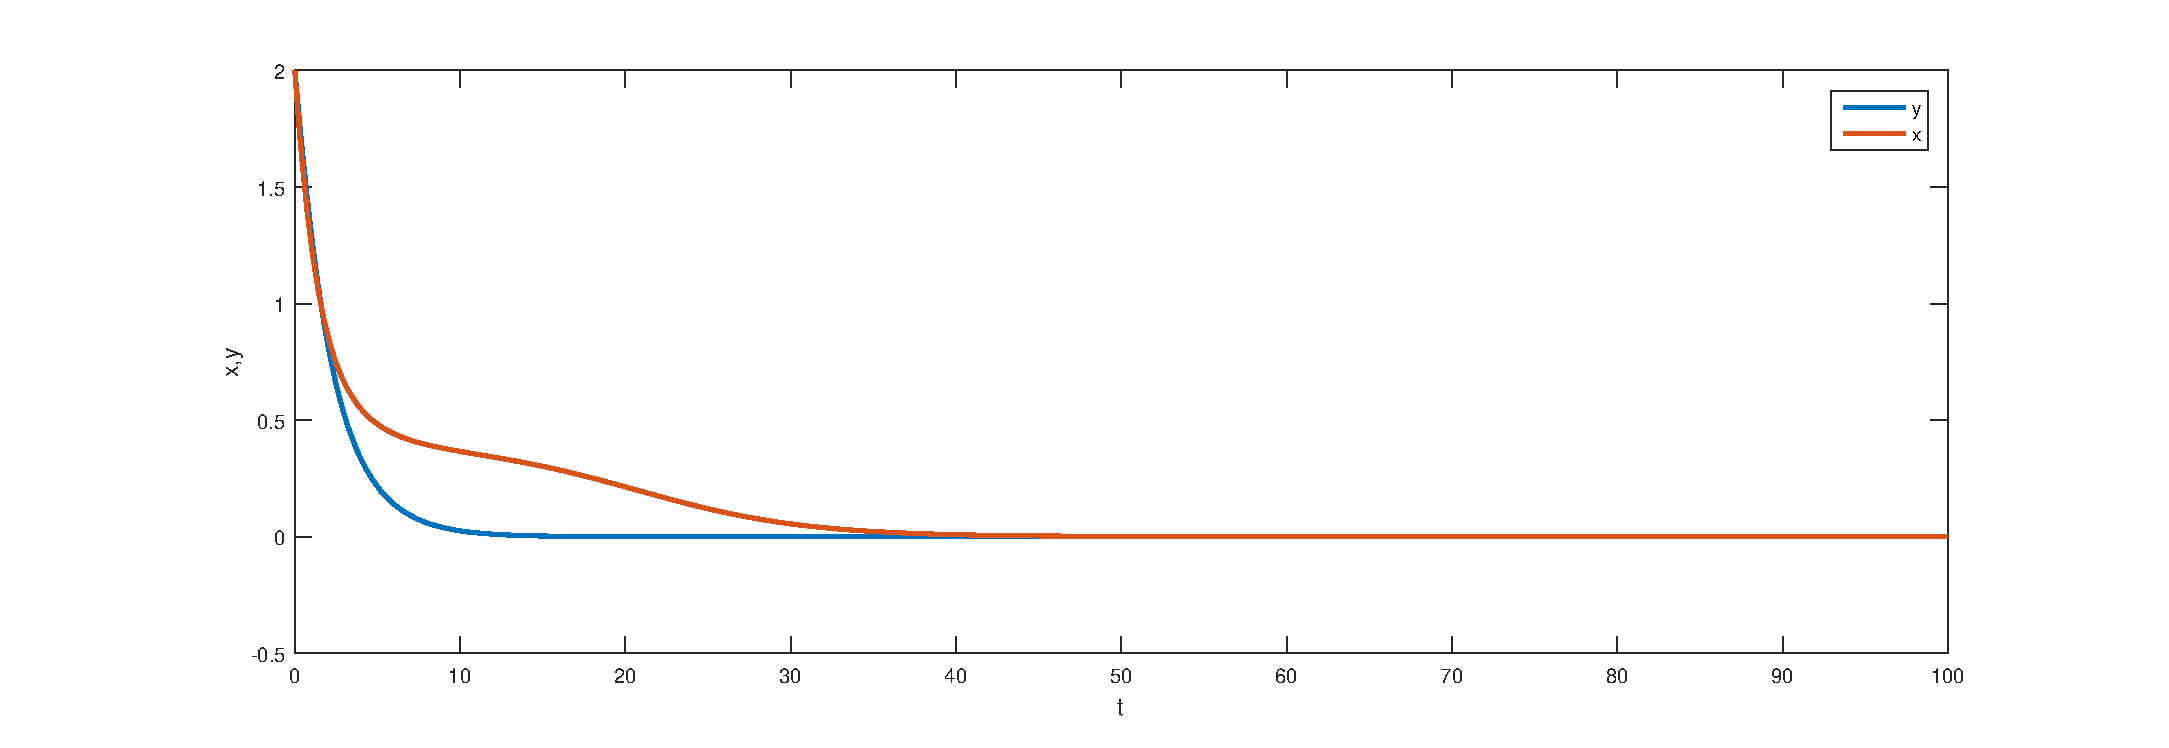
\includegraphics[width=9cm, height=6cm]{19a.eps}}
	\endminipage\hfill
	\minipage{0.5\textwidth}
	{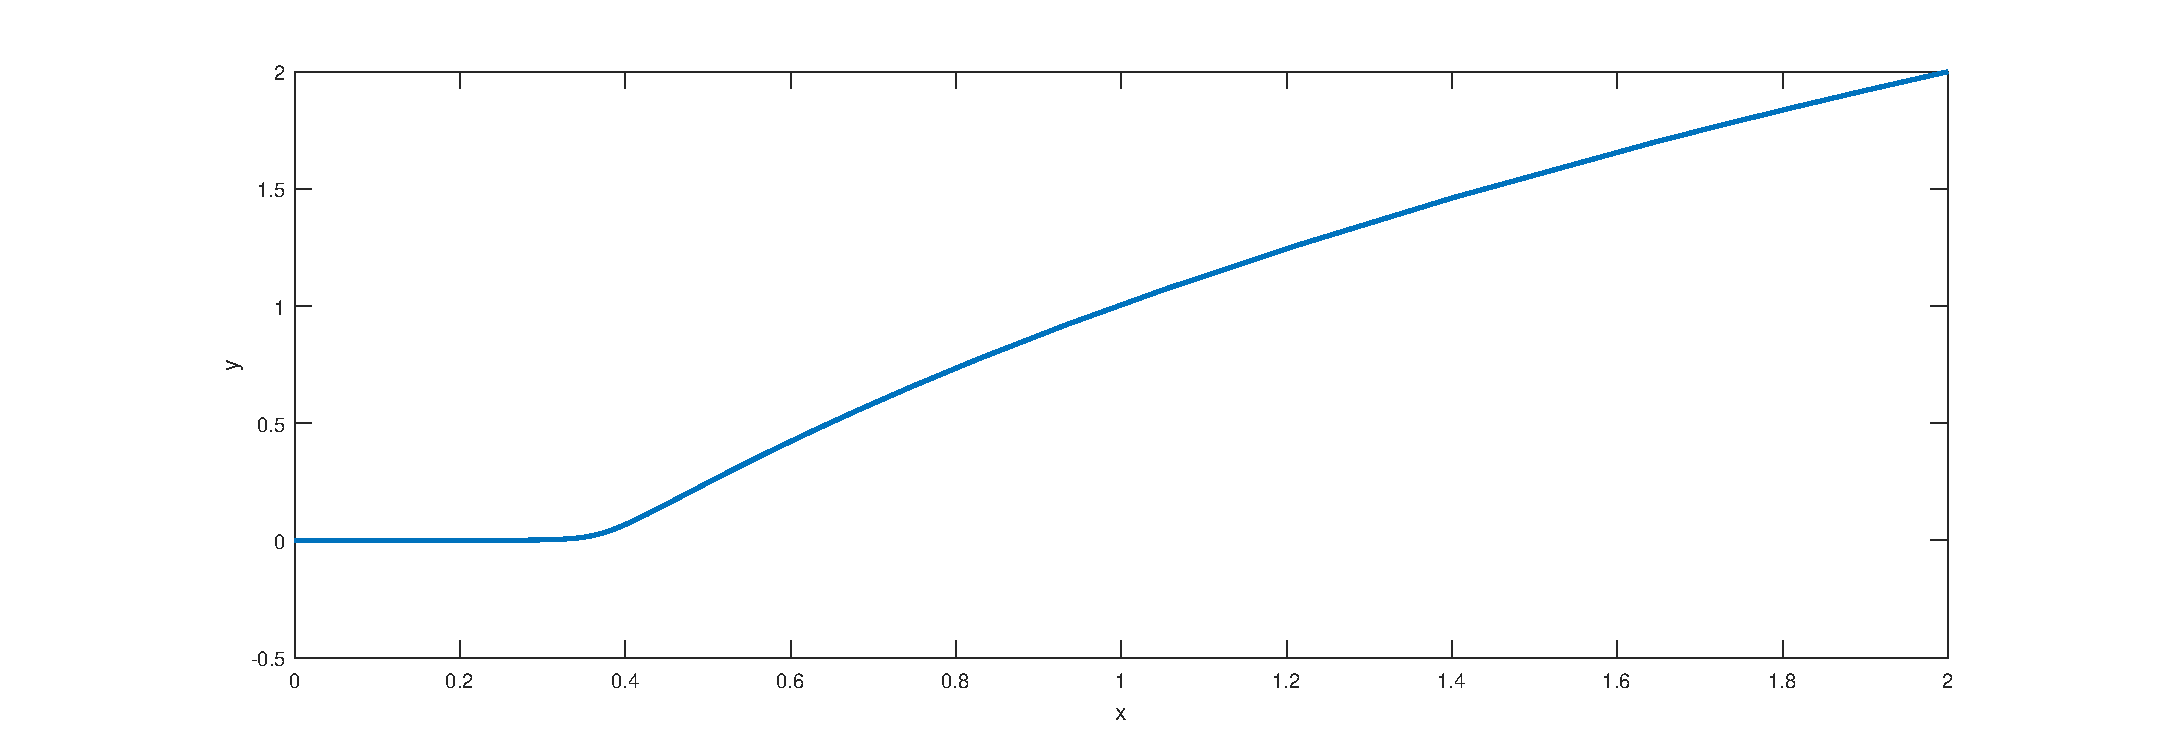
\includegraphics[width=9cm, height=6cm]{19b.eps}}
	\endminipage\hfill
	\begin{center} Figure 12: (a)Time series of $x,y$  (b)  of $y$ vs $x$ for extinction of the system for parameter $\delta_0$   \end{center}
\end{figure}  
From fig. 12 we see that the system that at $\delta_0=\delta_0^**=0.6$ and values of other parameters are same as in (8), the system stablilizes to the trivial equilibrium point solution and hence becomes extinct. 

Also in model (2), the parameter $\delta_1$ is also important because it tells us about about the intraspecific interference among the predators. Therefore we will analyze how the dynamics of system changes with respect to $\delta_1$ by using Hopf-bifurcation analysis.
\begin{figure}[H]
	\minipage{0.5\textwidth}
	{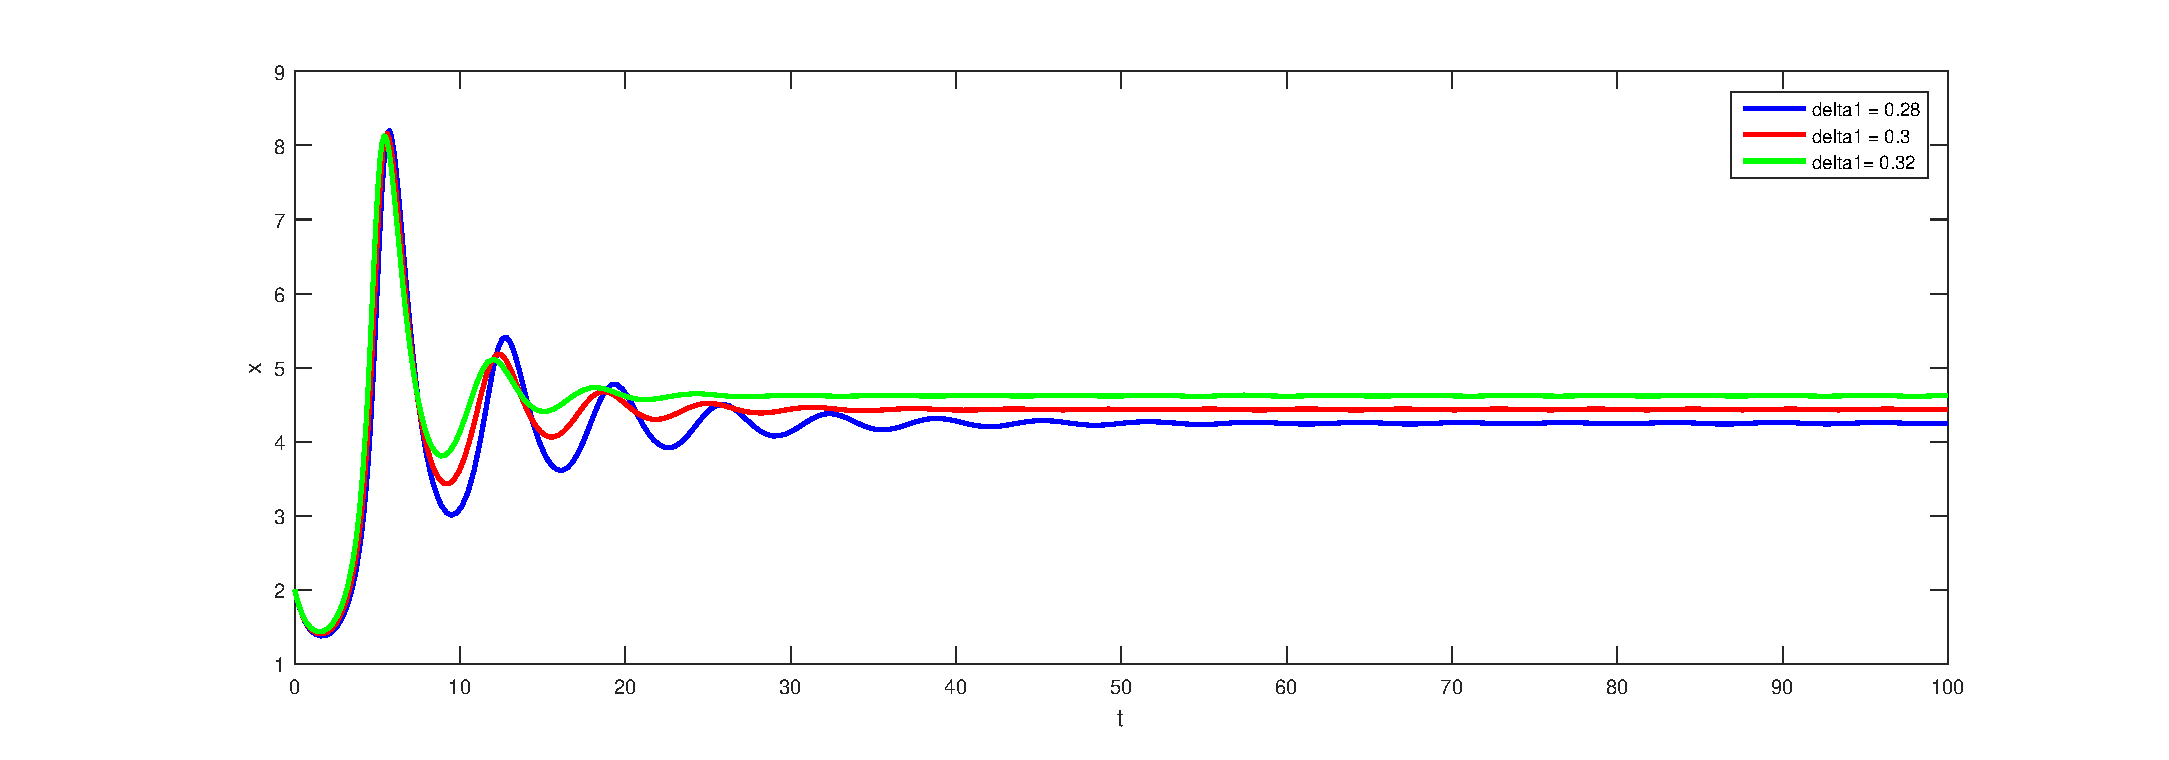
\includegraphics[width=9cm, height=6cm]{20a.eps}}
	\endminipage\hfill
	\minipage{0.5\textwidth}
	{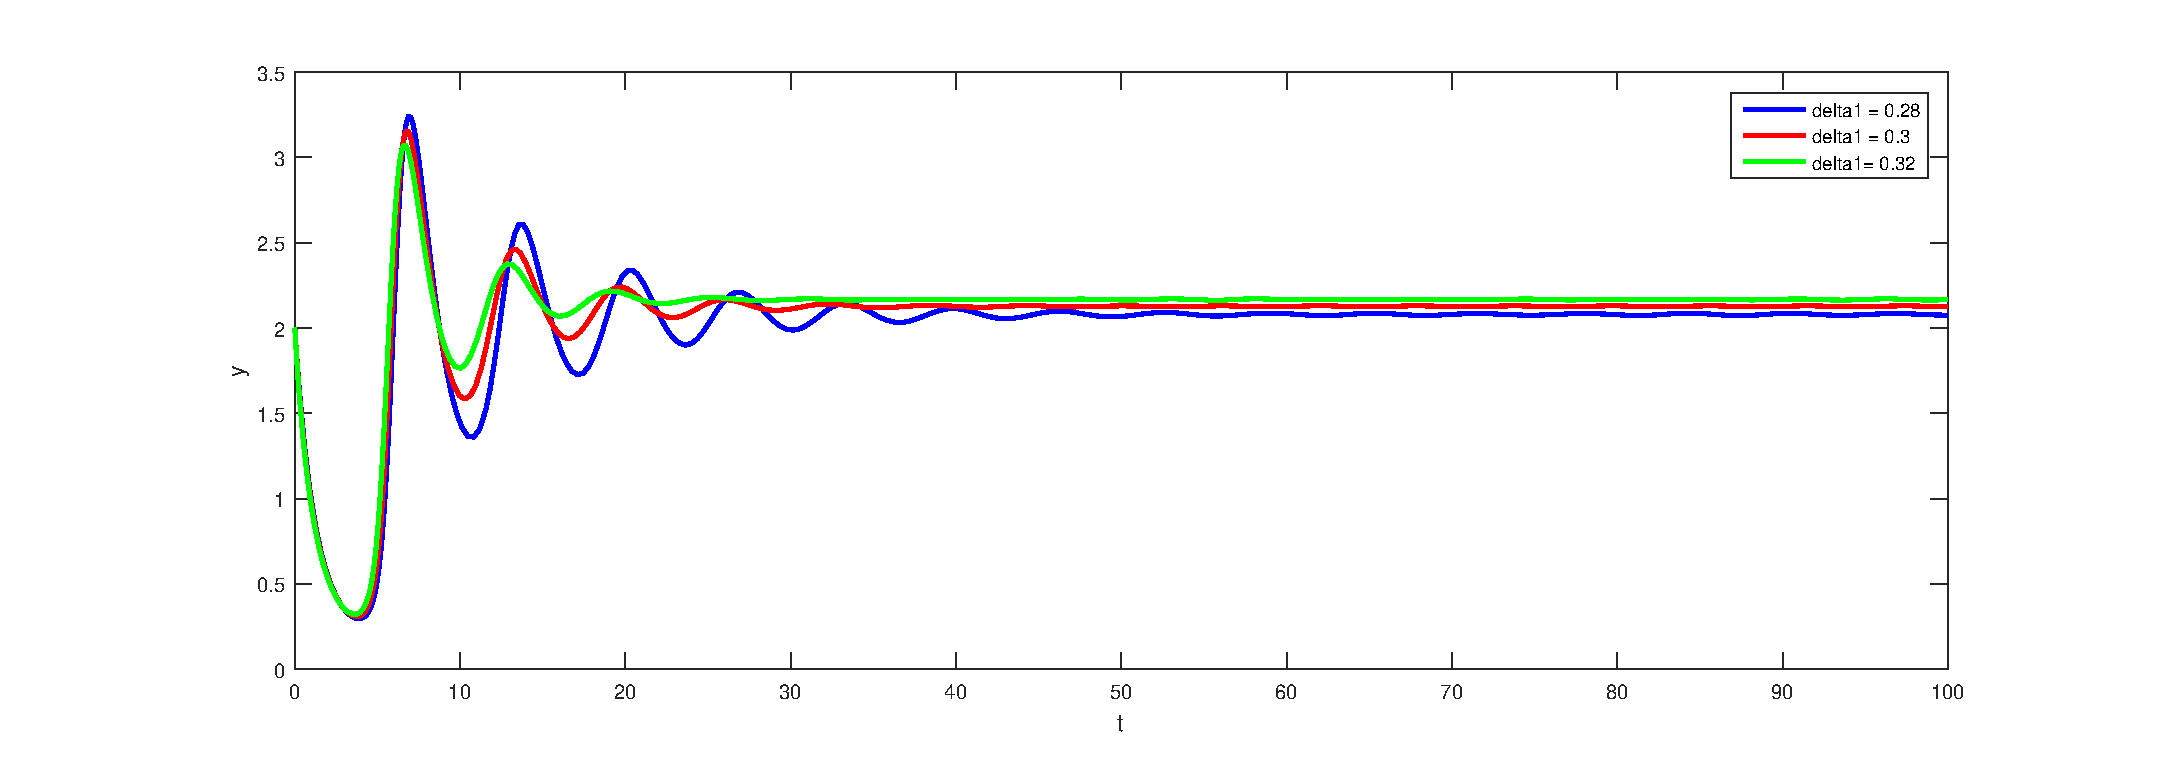
\includegraphics[width=9cm, height=6cm]{20b.eps}}
	\endminipage\hfill
	\begin{center} Figure 13: (a)Time series of $x$  (b) Time series of $y$  for different values of parameter $\delta_0$   \end{center}
\end{figure}
From figure 10, we observe that as $\delta_1$ increases the system gains stability.
\begin{figure}[H]
	\minipage{0.5\textwidth}
	{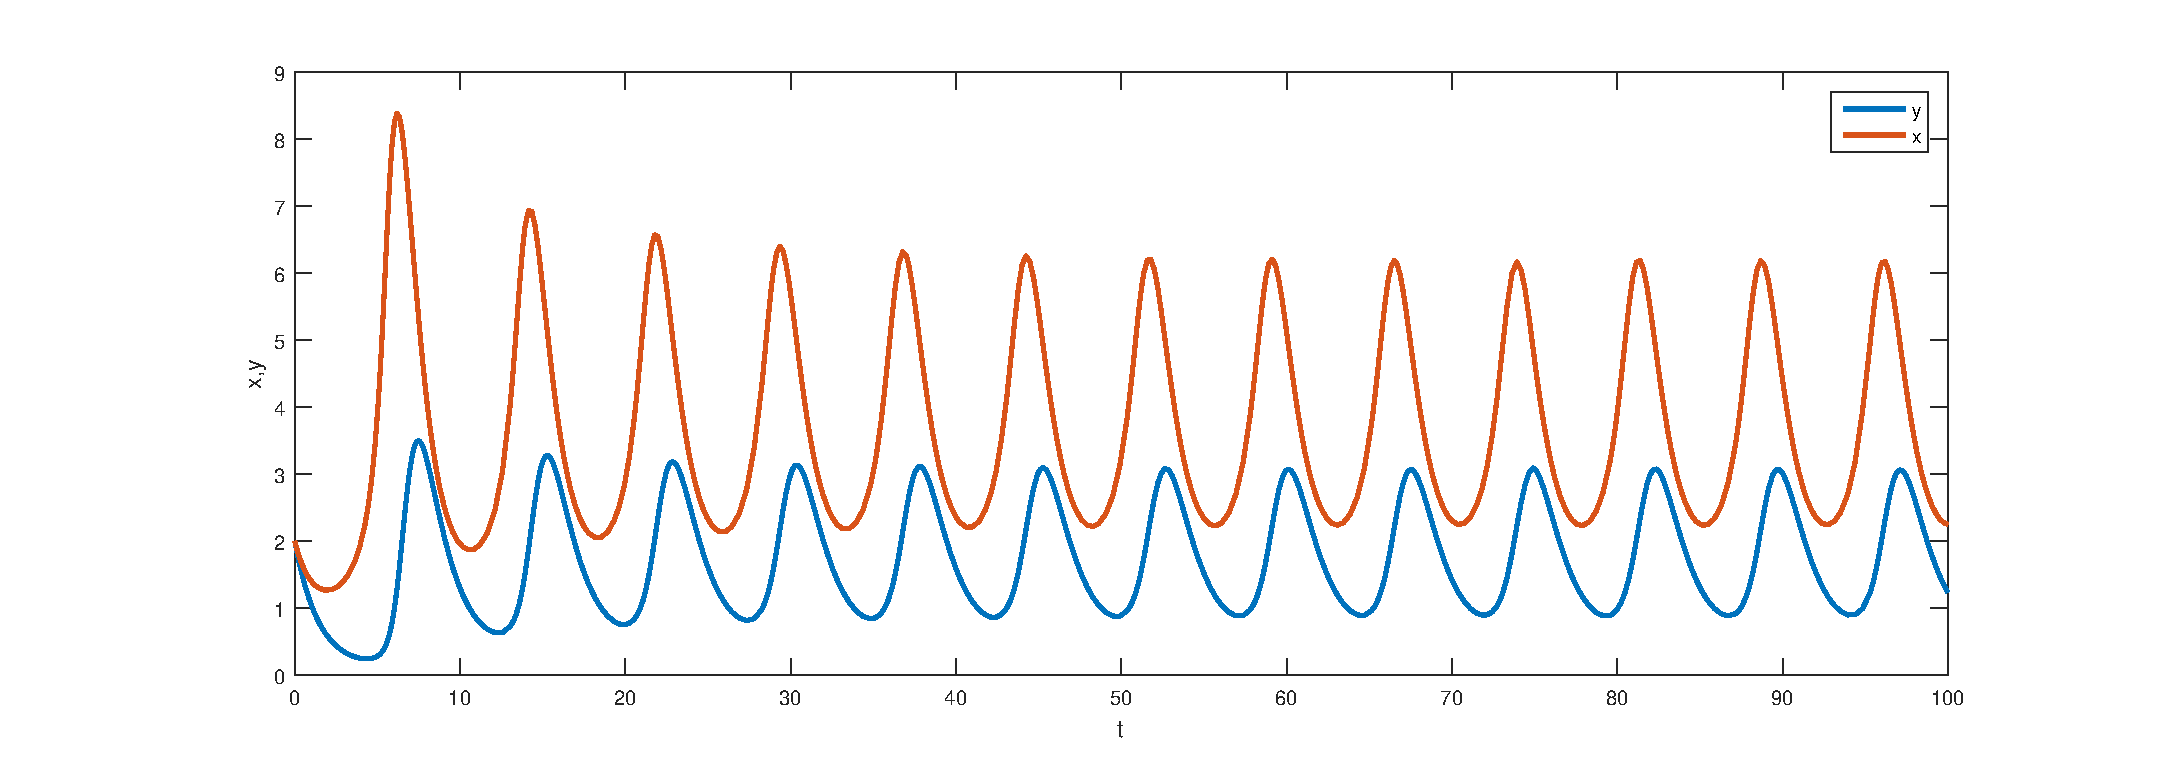
\includegraphics[width=9cm, height=6cm]{21a.eps}}
	\endminipage\hfill
	\minipage{0.5\textwidth}
	{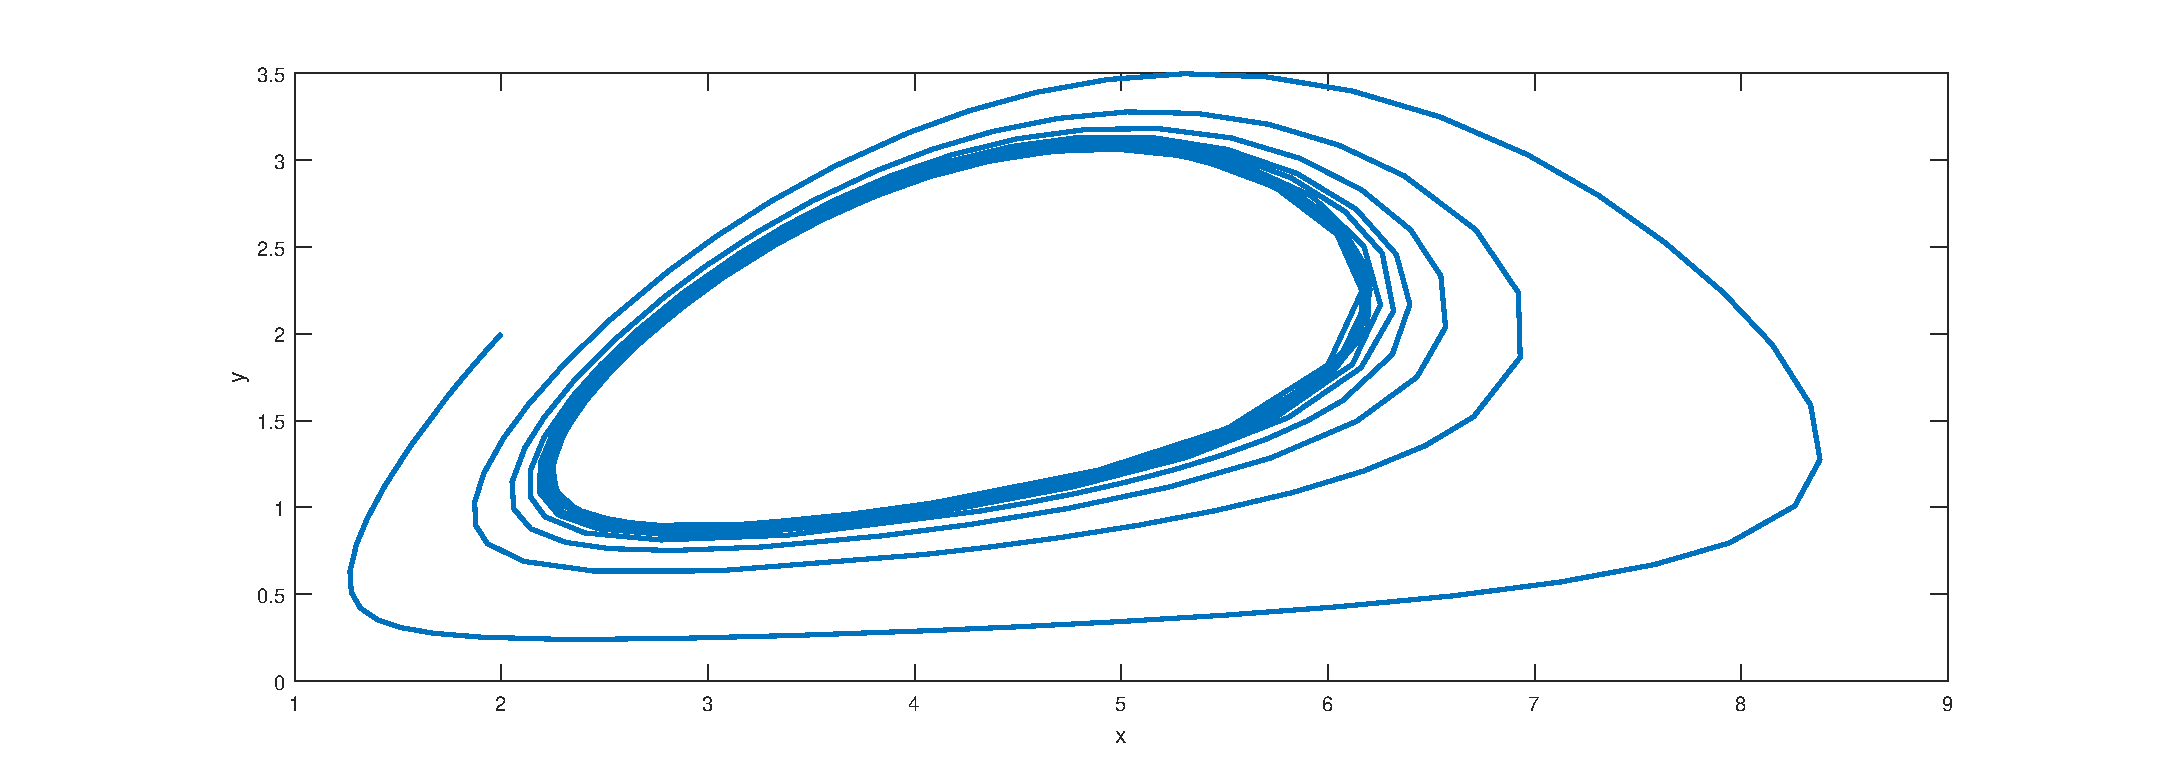
\includegraphics[width=9cm, height=6cm]{21b.eps}}
	\endminipage\hfill
	\begin{center} Figure 14: (a)Time series of $x,y$  (b)  of $y$ vs $x$ for Hopf-Bifurcation of parameter $\delta_1$   \end{center}
\end{figure}
The system (2) shows Hopf-bifurcation at $\delta_1=\delta_1^*=0.25$ and values of other parameters are same as in (8). In figure 11 we depicted time series (Fig. 14(a)) and phase portrait of the system (Fig. 14(b)) for $\delta_1=0.2~\textless~\delta_1^*=0.25,$ which refers that the system (2) has periodic solutions.
\begin{figure}[H]
	\minipage{0.5\textwidth}
	{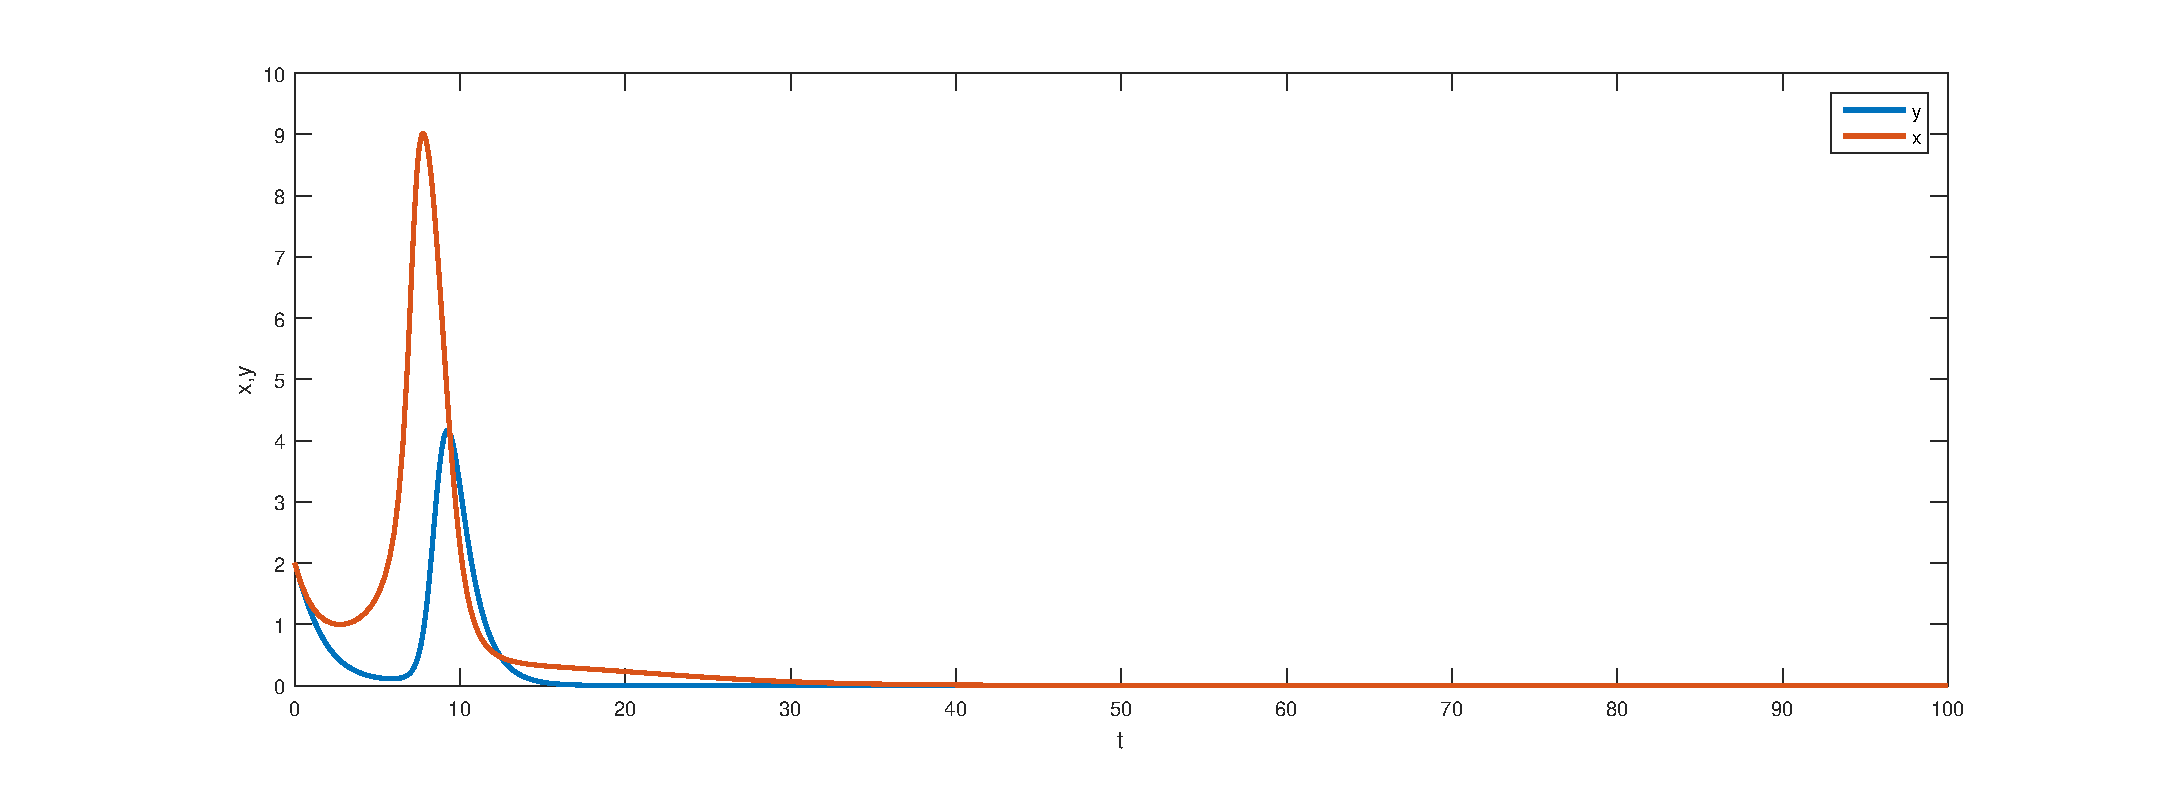
\includegraphics[width=9cm, height=6cm]{22a.eps}}
	\endminipage\hfill
	\minipage{0.5\textwidth}
	{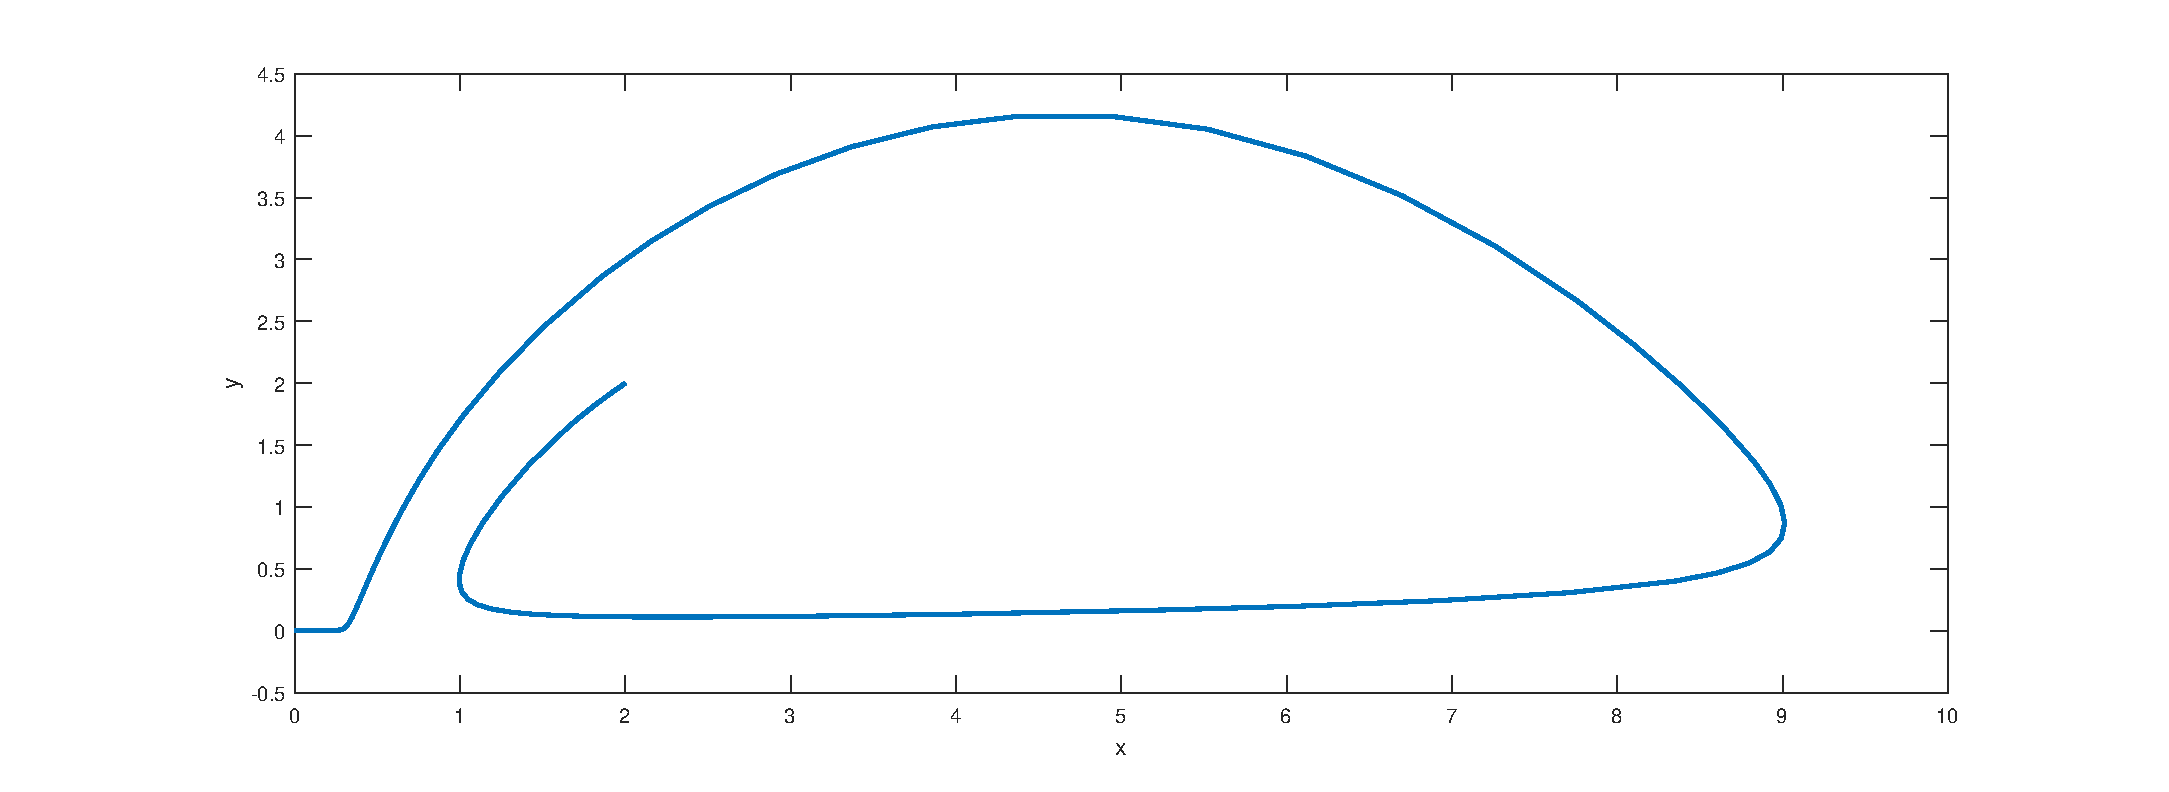
\includegraphics[width=9cm, height=6cm]{22b.eps}}
	\endminipage\hfill
	\begin{center} Figure 15: (a)Time series of $x,y$  (b)  of $y$ vs $x$ for extinction of the system for parameter $\delta_1$   \end{center}
\end{figure}  
From fig. 12 we see that the system that at $\delta_1=\delta_1^**=0.13$ and values of other parameters are same as in (8), the system stablilizes to the trivial equilibrium point solution and hence becomes extinct.
\subsubsection{Weak Allee case}
For the model (3), we consider a set of parameters as follows:
\begin{equation}
\begin{split}
& r=2,~K=50,~\theta=4,~\alpha=0.7,\\
& a=0.04,~b=0.07,~c=0.7,~\delta_0=1,~\delta_1=0.3,
\end{split}
\end{equation}
with initial conditions $x(0)=y(0)=2.$
\begin{figure}[H]
	\minipage{0.5\textwidth}
	{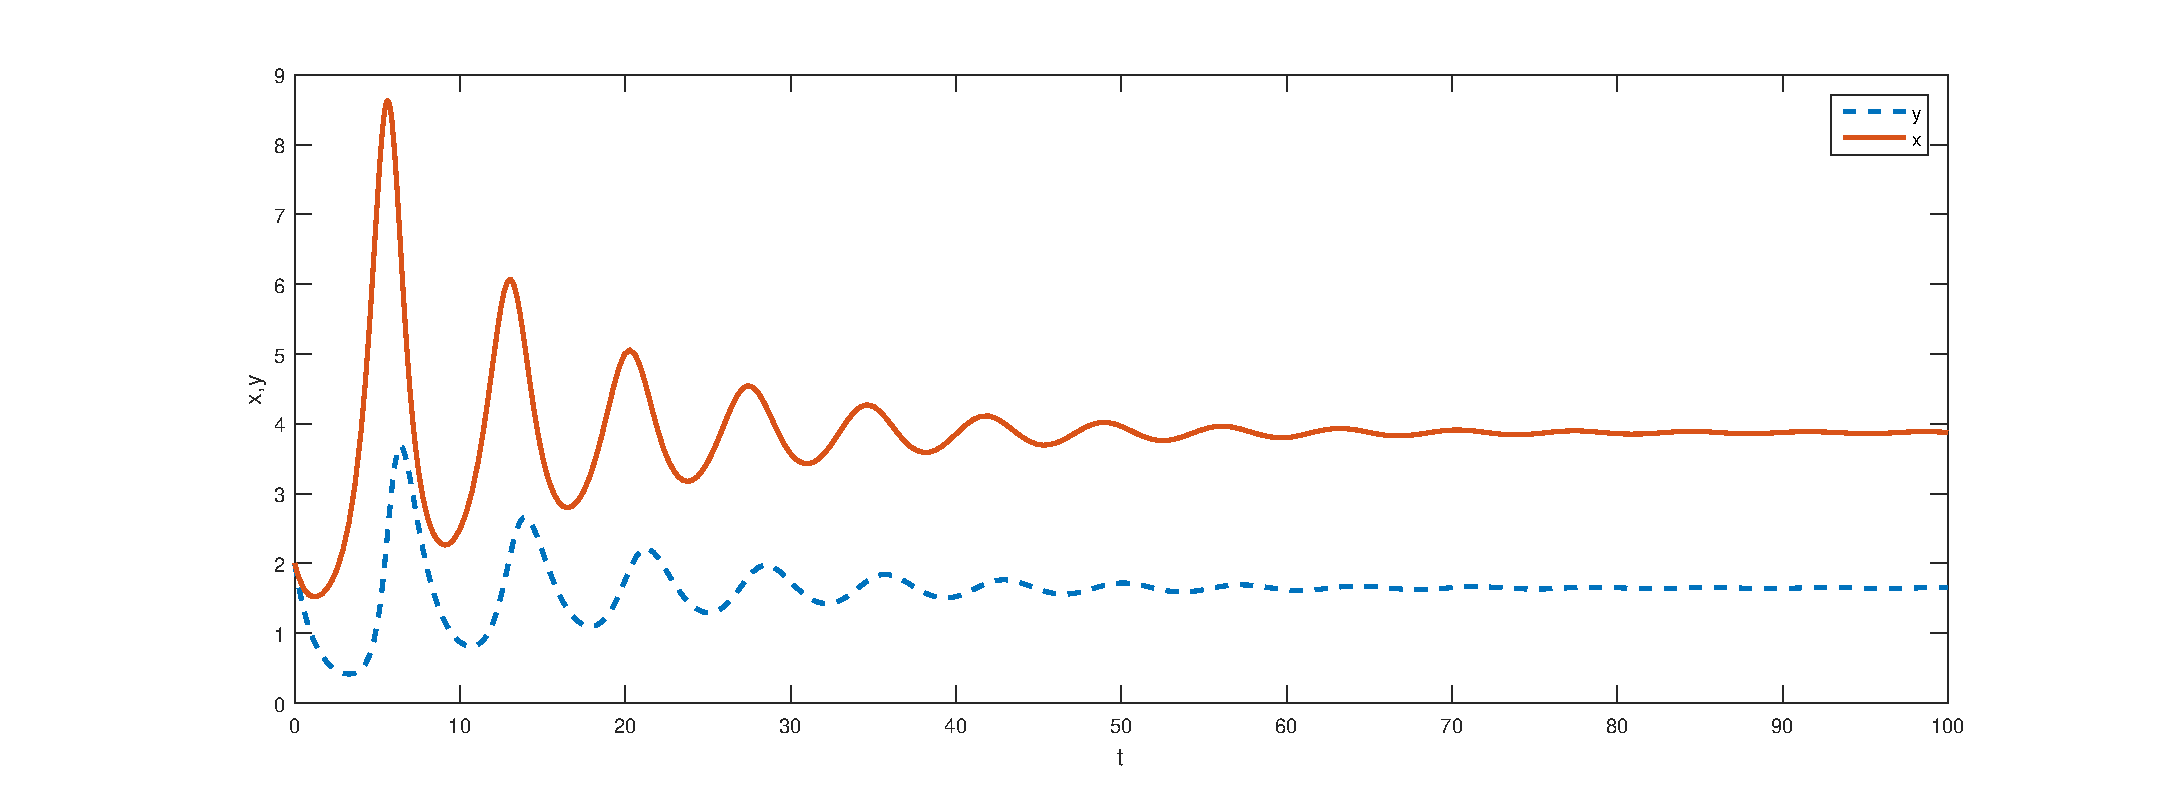
\includegraphics[width=9cm, height=6cm]{23a.eps}}
	\endminipage\hfill
	\minipage{0.5\textwidth}
	{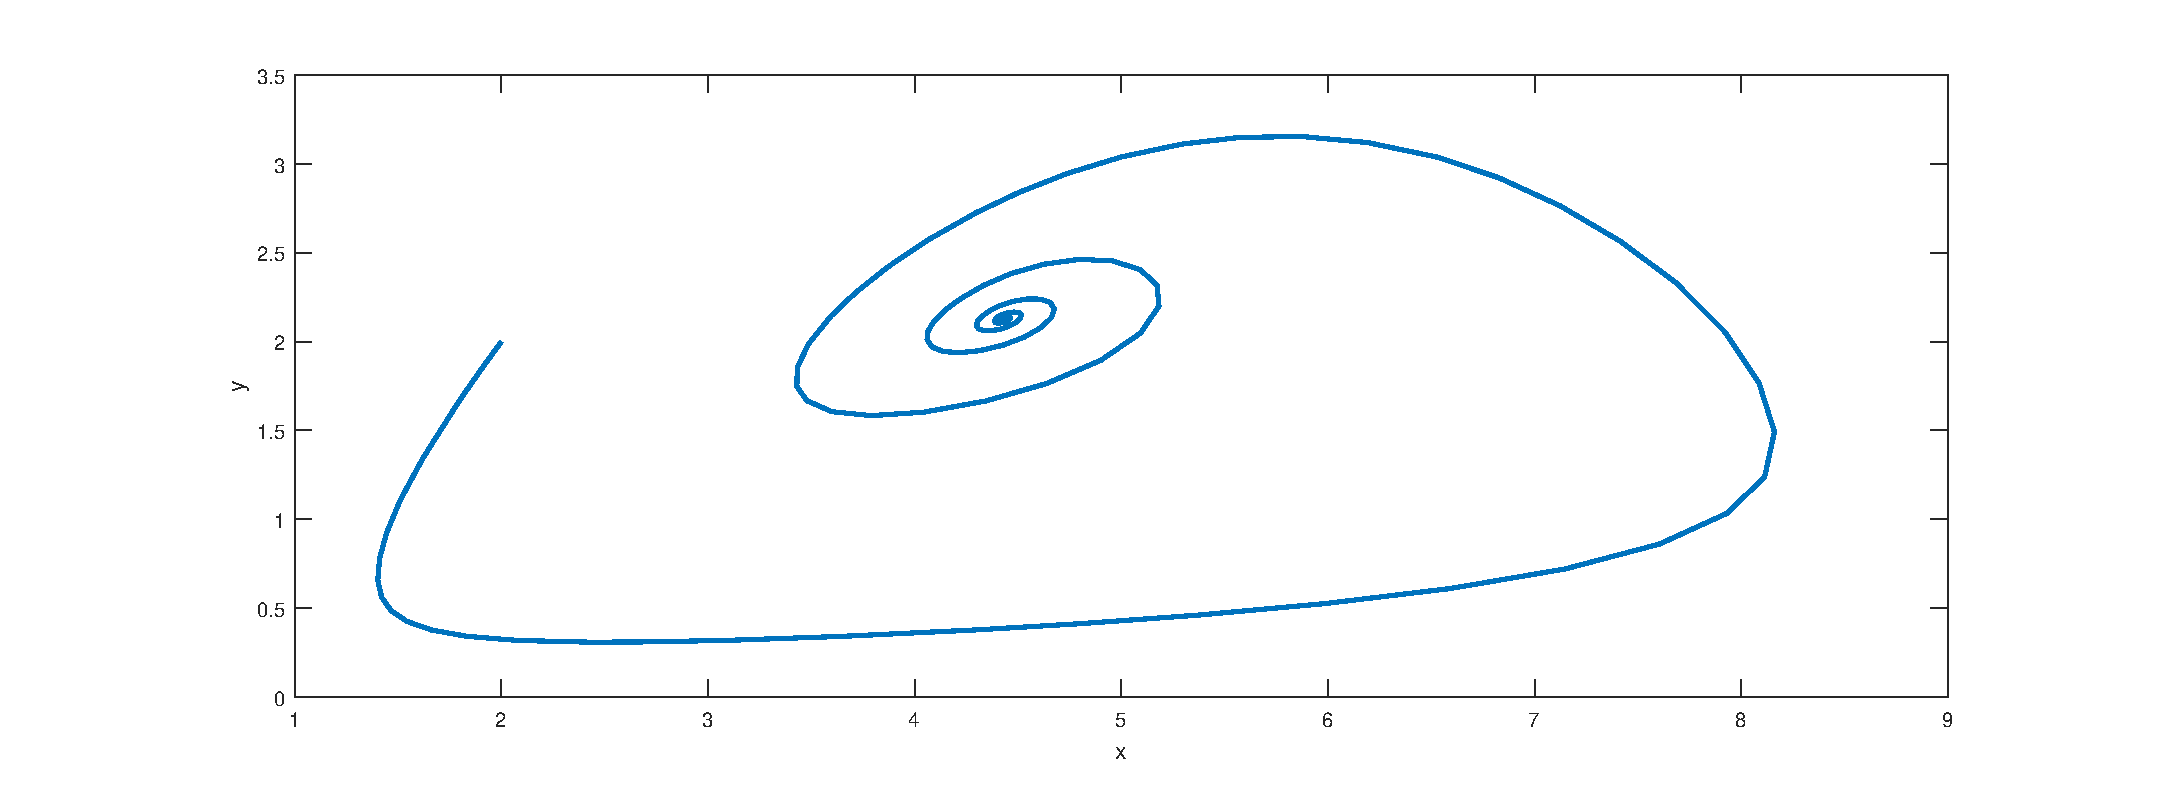
\includegraphics[width=9cm, height=6cm]{23b.eps}}
	\endminipage\hfill
	\begin{center} Figure 16: Time series of $x$ and $y$ (a) and phase portrait (b) for $\theta=4~\textless~\theta_*.$ $E_*$ is asymptotically stable.  \end{center}
\end{figure}
On the other hand the system (3), with weak Allee effect in prey population, with same values of parameters condition (8) holds true. Therefore system has only one interior equilibrium point $E_*(3.8732,1.6471)$. The system (3) also exhibits Hopf-bifurcation but the threshold value of $\theta$ moves on $\theta_*=4.54.$ Hence the system is stable when $\theta=4 ~\textless~\theta_*$ (fig. 17) and shows periodic solution when  $\theta=6~\textgreater~\theta_*$ (fig. 9).
\begin{figure}[H]
	\minipage{0.5\textwidth}
	{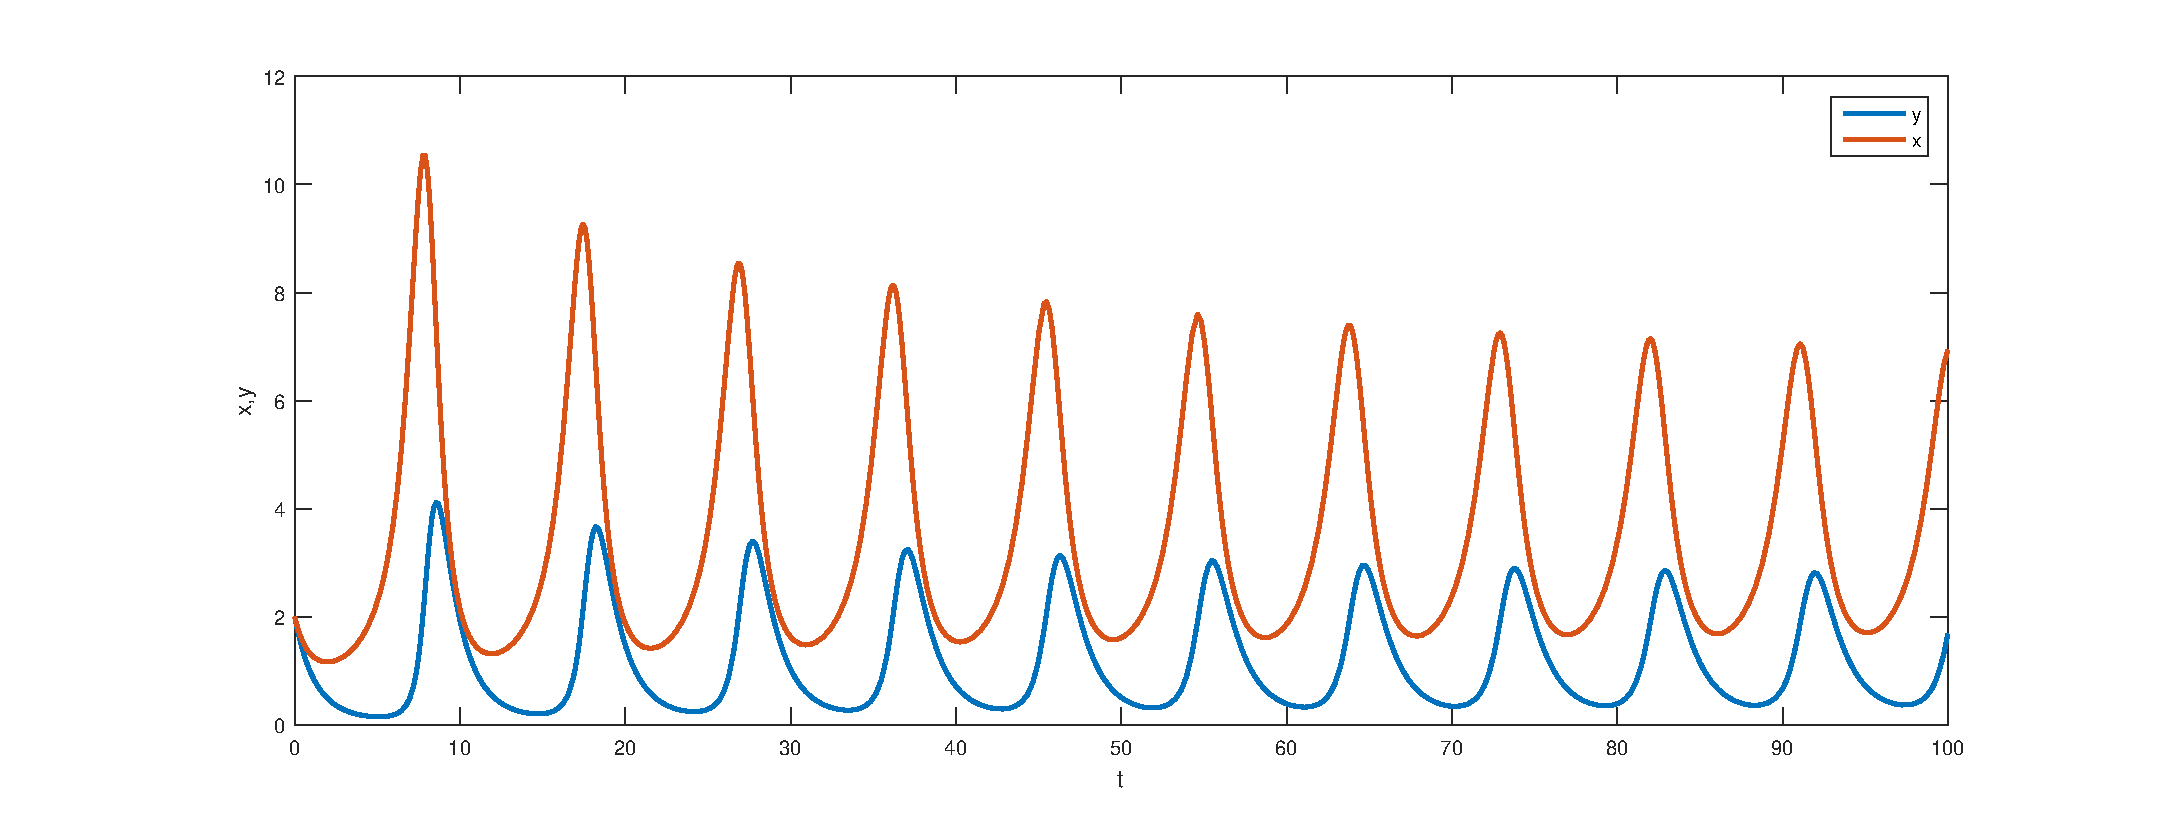
\includegraphics[width=9cm, height=6cm]{24a.eps}}
	\endminipage\hfill
	\minipage{0.5\textwidth}
	{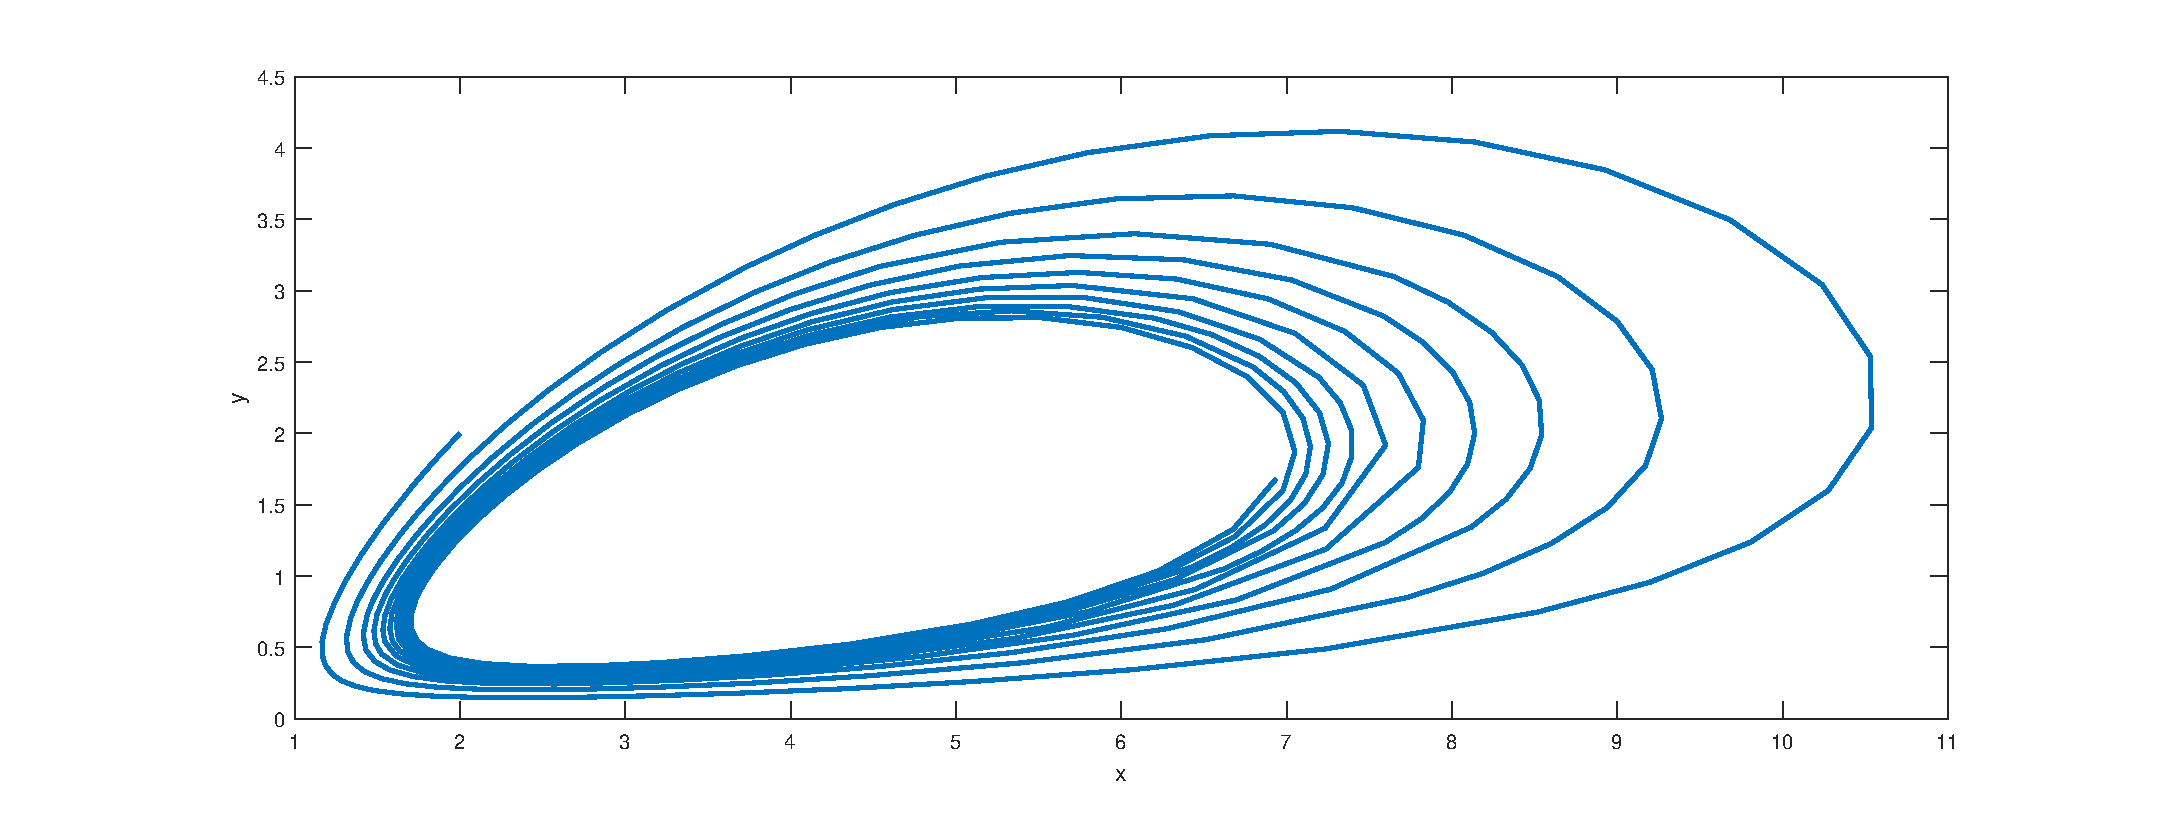
\includegraphics[width=9cm, height=6cm]{24b.eps}}
	\endminipage\hfill
	\begin{center} Figure 17: Time series of $x$ and $y$ (a) and existence of periodic solution (b) for $\theta=6~\textgreater~\theta_*.$   \end{center}
\end{figure}
The bifurcation diagram has been shown in figure 10(a-b) by taking $\theta$ as a bifurcation parameter. This figure depicts the dynamics of the system as the Allee parameter increases. From the figure, it is evident that $\theta~\textless~\theta_*,$ the system (3) is stable but as $\theta$ crosses its critical value, the system exibits periodic solutions.
\begin{figure}[H]
	\minipage{0.5\textwidth}
	{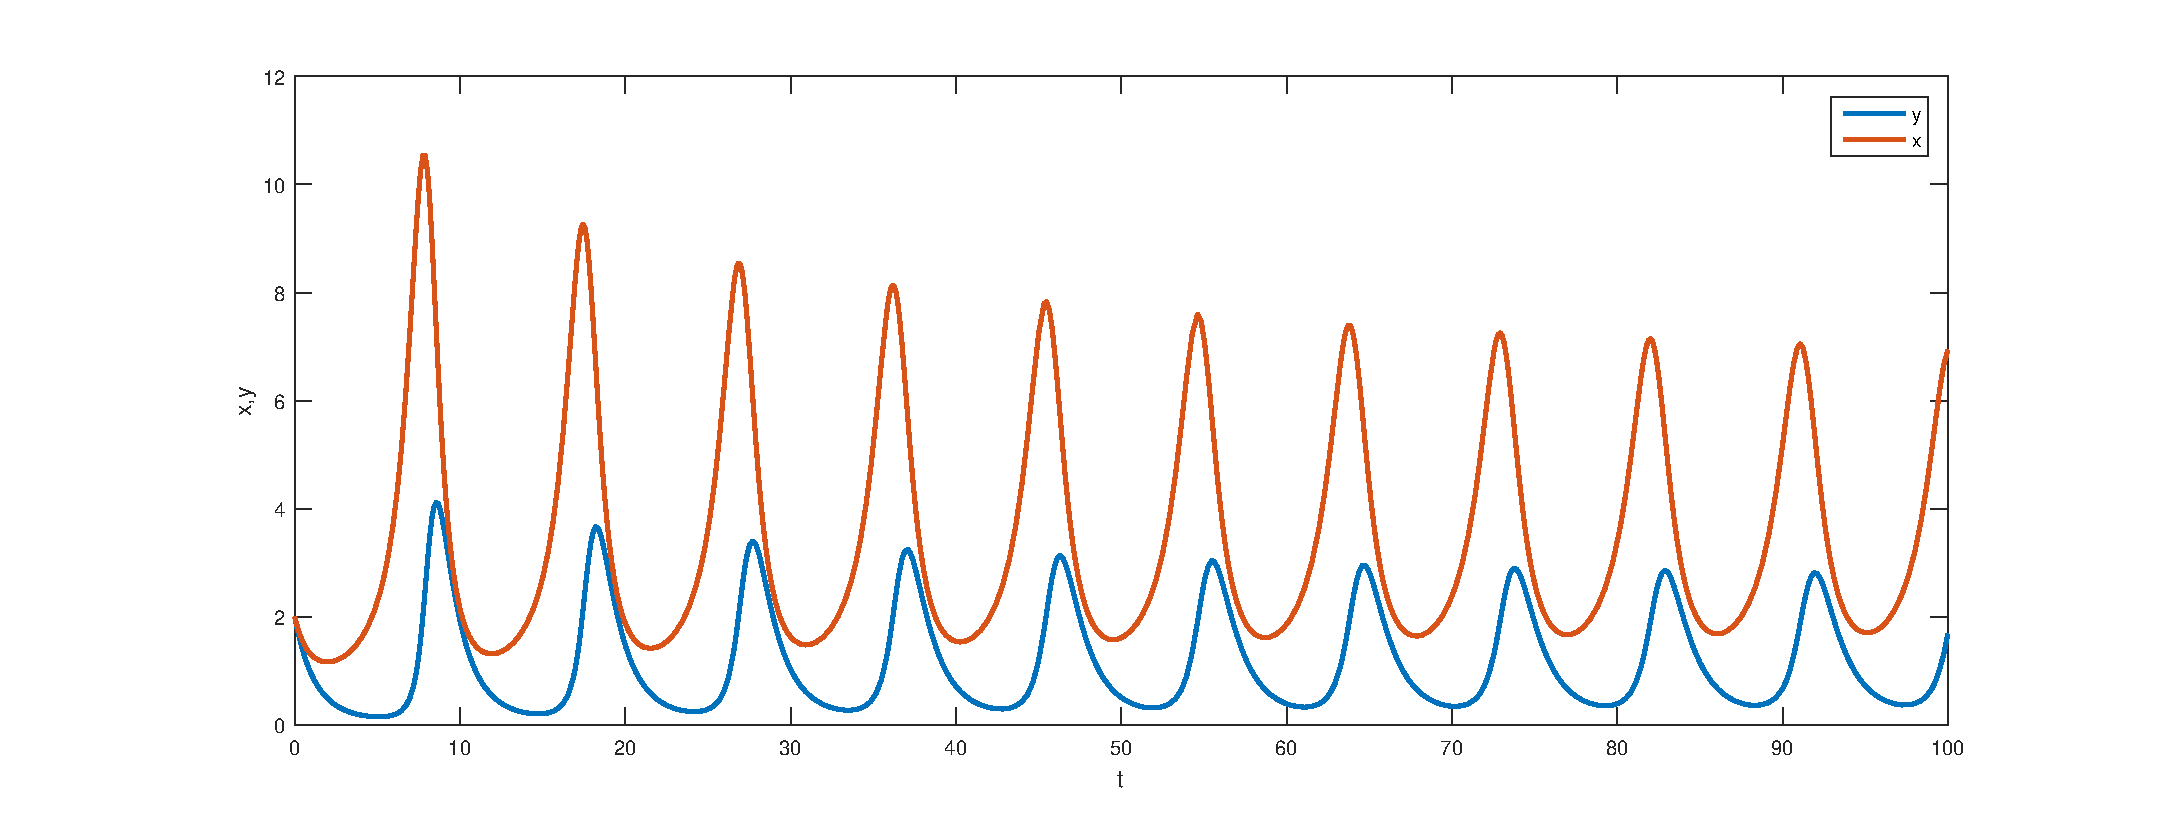
\includegraphics[width=9cm, height=6cm]{24a.eps}}
	\endminipage\hfill
	\minipage{0.5\textwidth}
	{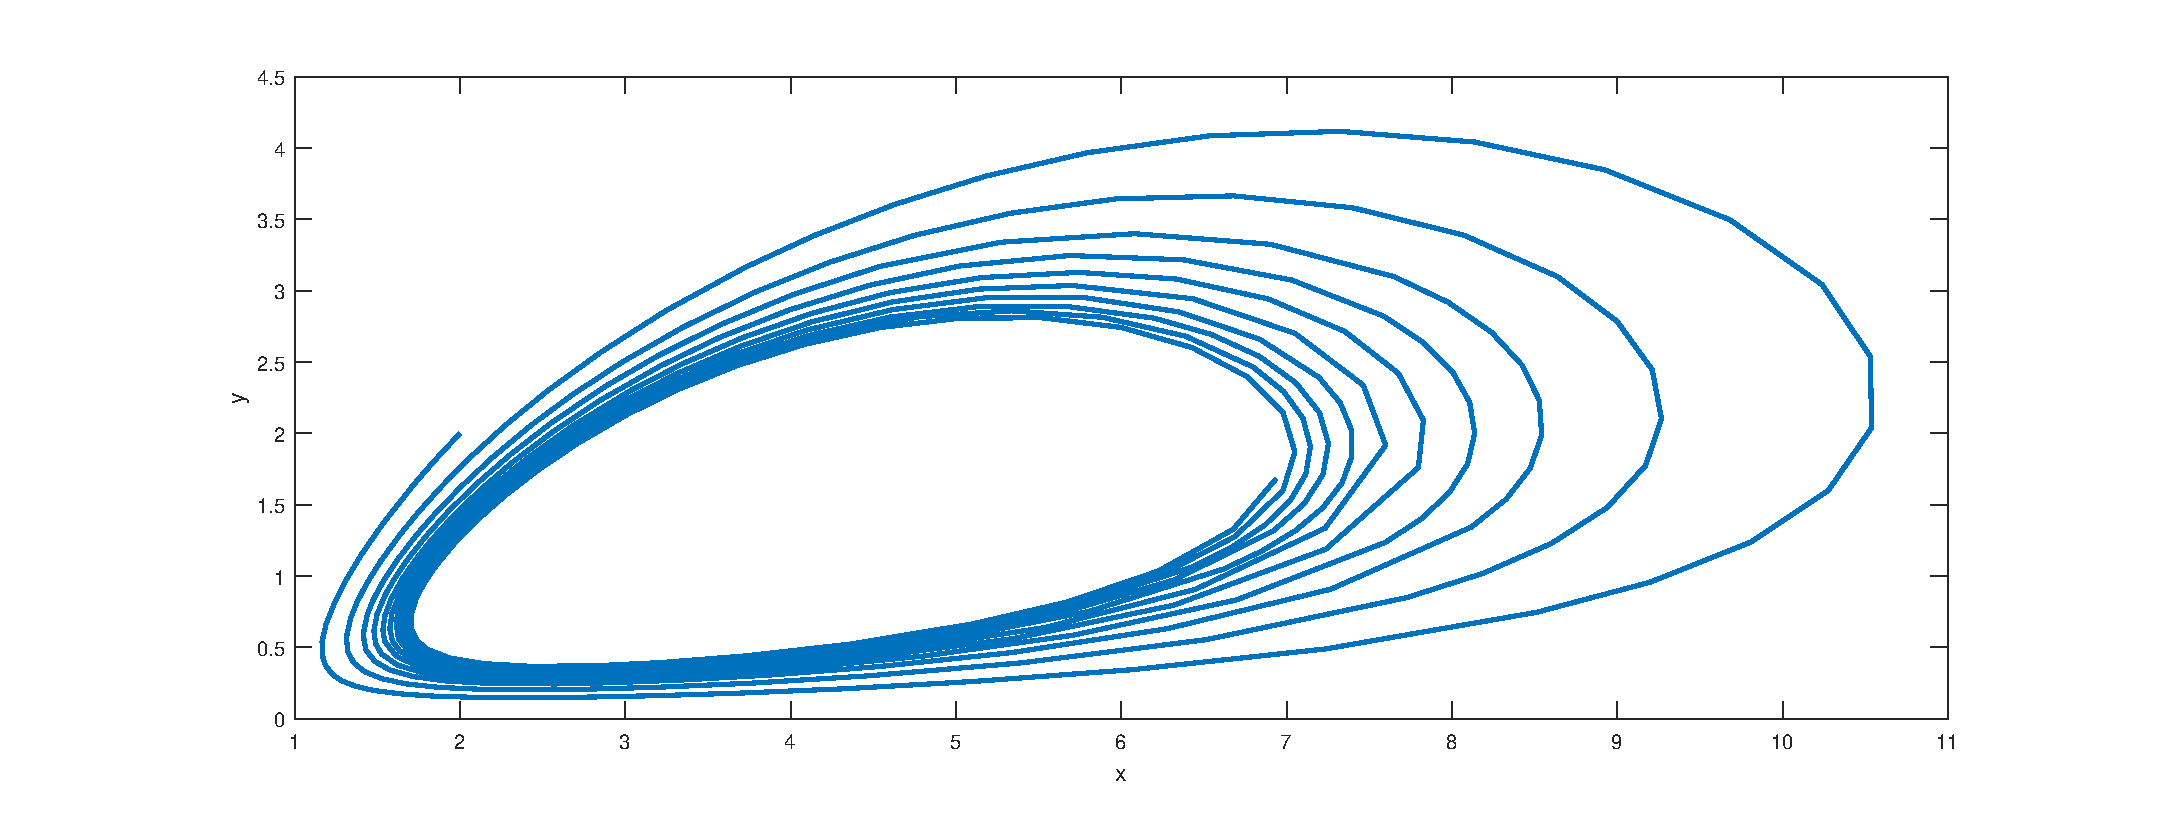
\includegraphics[width=9cm, height=6cm]{24b.eps}}
	\endminipage\hfill
	\begin{center} Figure 18: Bifurcation diagram of the prey and predator population with respect to Allee parameter $\theta.$  \end{center}
\end{figure}

\begin{figure}[H]
	\minipage{0.5\textwidth}
	{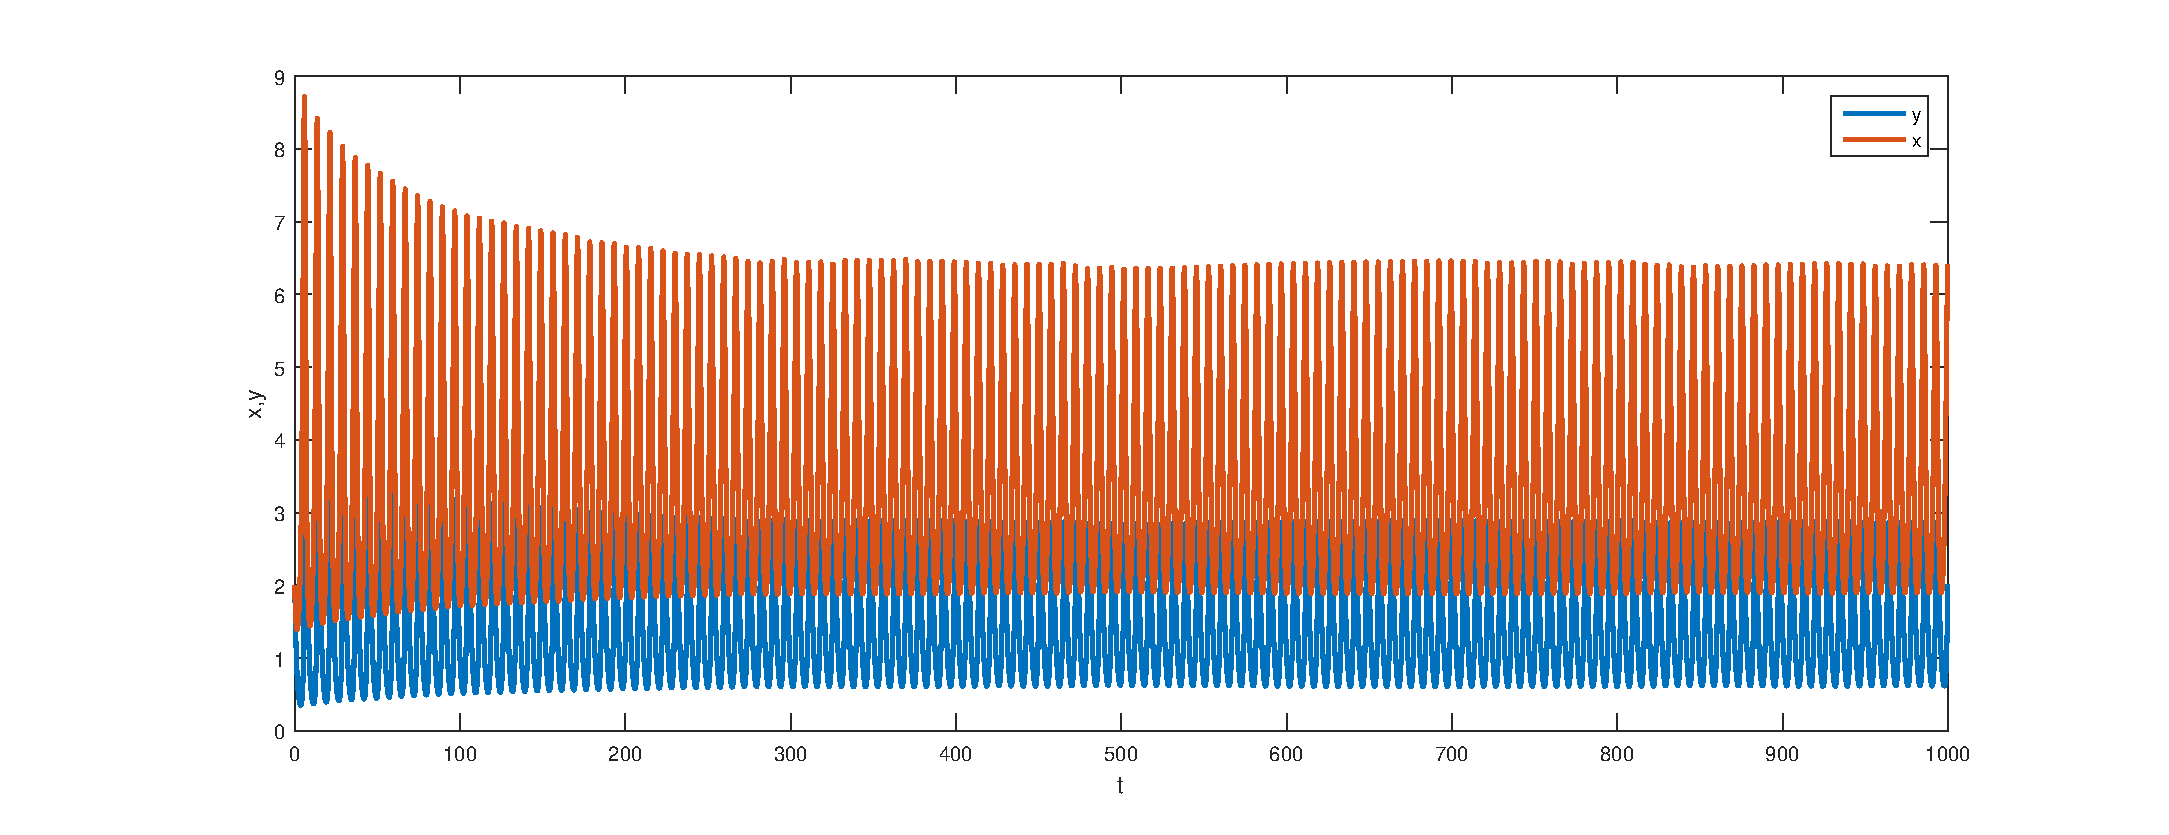
\includegraphics[width=9cm, height=6cm]{25a.eps}}
	\endminipage\hfill
	\minipage{0.5\textwidth}
	{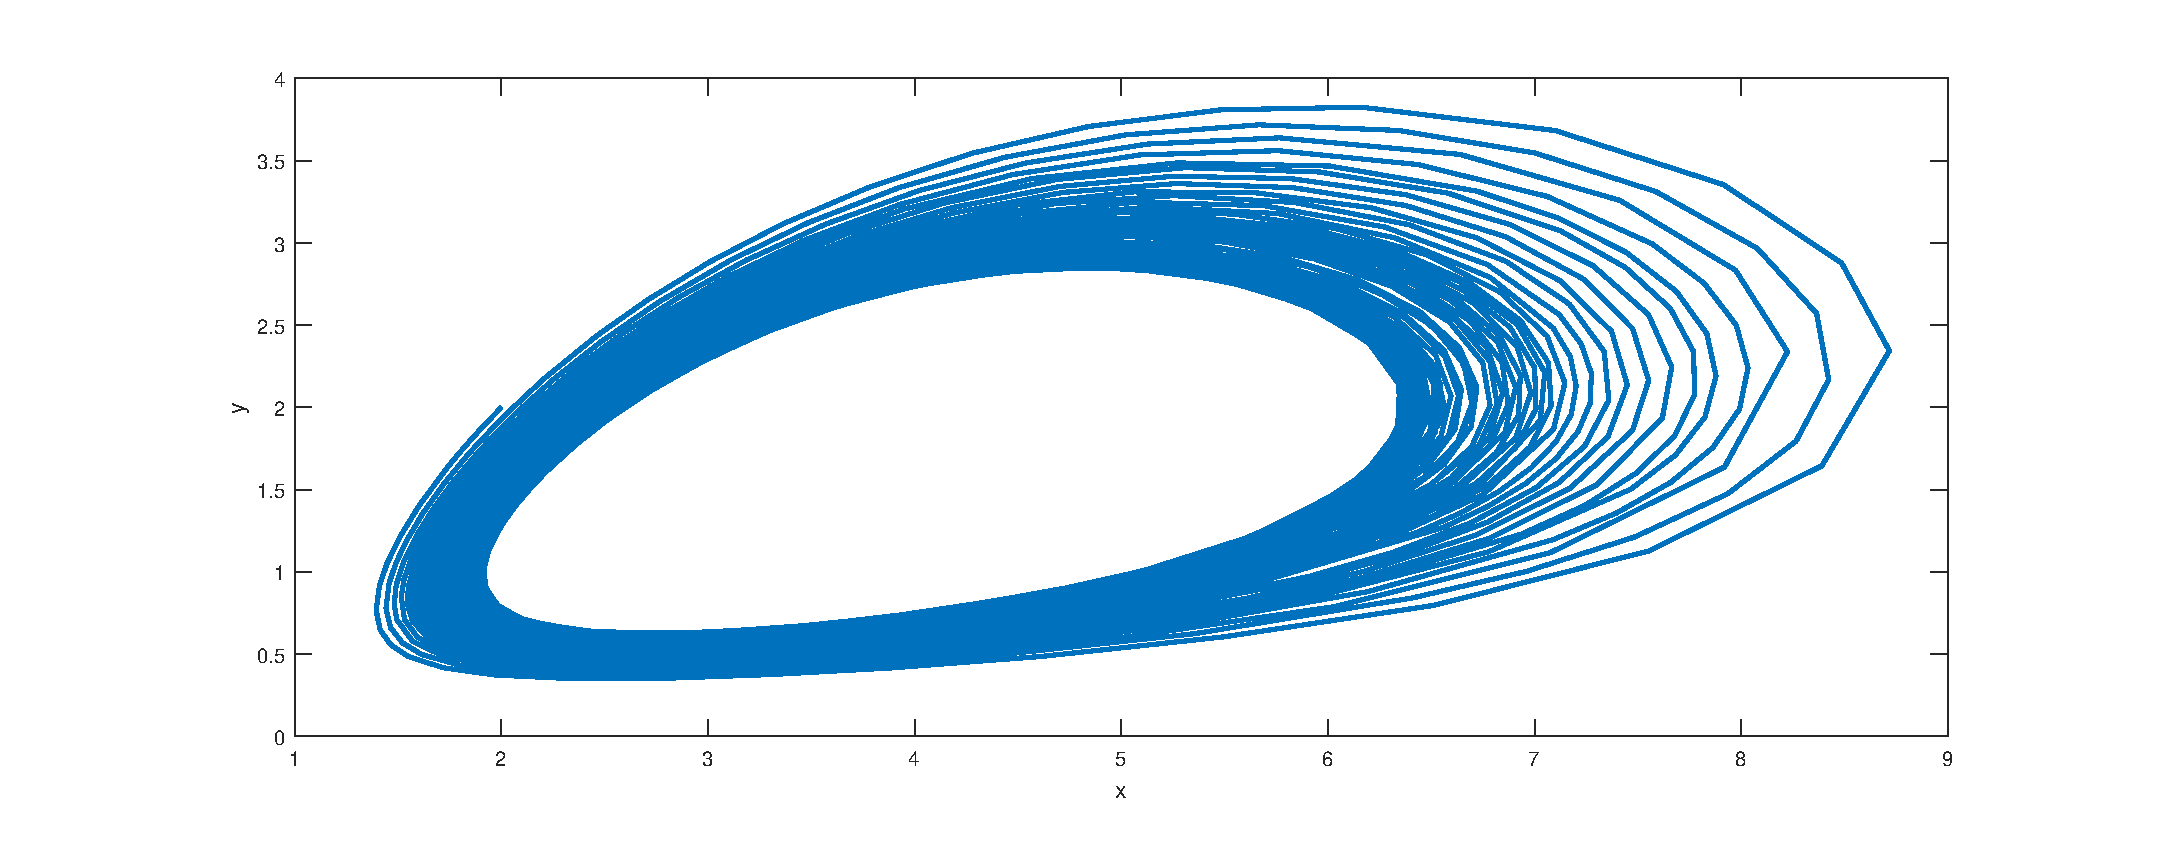
\includegraphics[width=9cm, height=6cm]{25b.eps}}
	\endminipage\hfill
	\begin{center} Figure 19: Time series of $x$ and $y$ (a) and phase portrait (b) for $b=0.03~\textless~b*.$ $E_*$ is unstable.  \end{center}
\end{figure}
From the figure, it is evident that $b~\textless~b^*,$ the system (3) is stable but as $b$ becomes less than its critical value($b^*=0.04$), the system shows periodic solutions.

\begin{figure}[H]
	\minipage{0.5\textwidth}
	{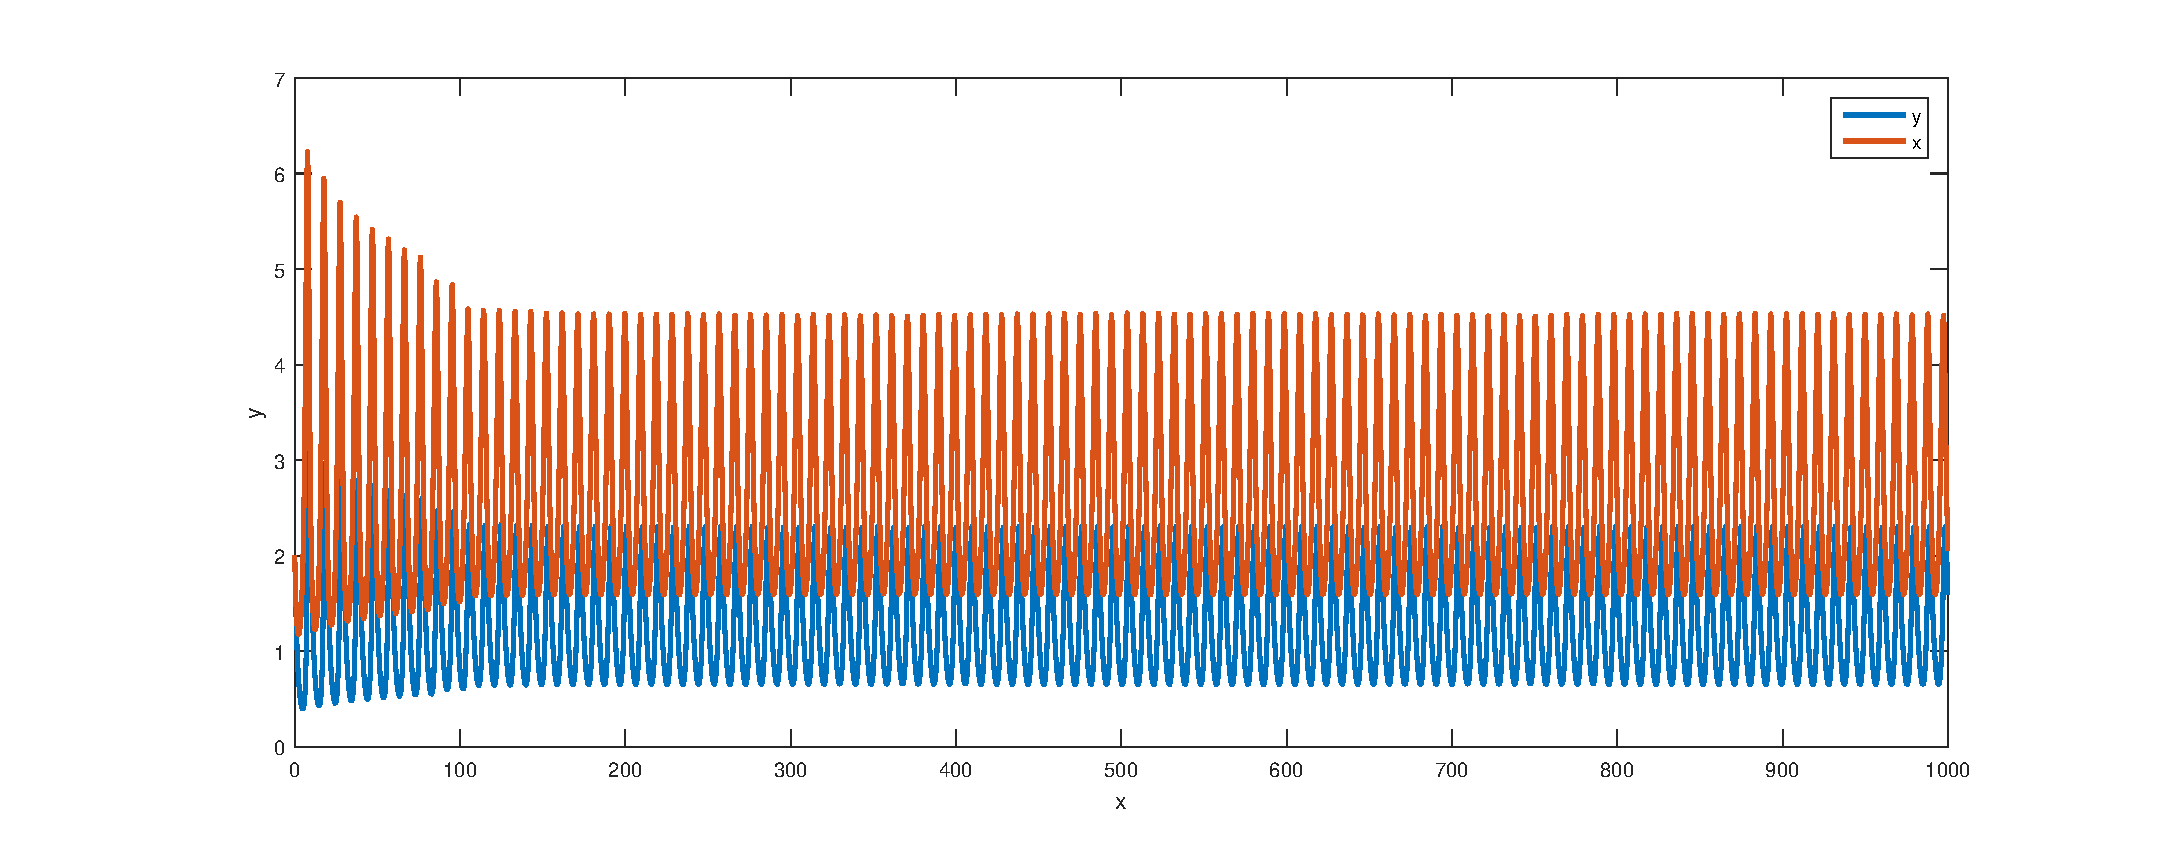
\includegraphics[width=9cm, height=6cm]{26a.eps}}
	\endminipage\hfill
	\minipage{0.5\textwidth}
	{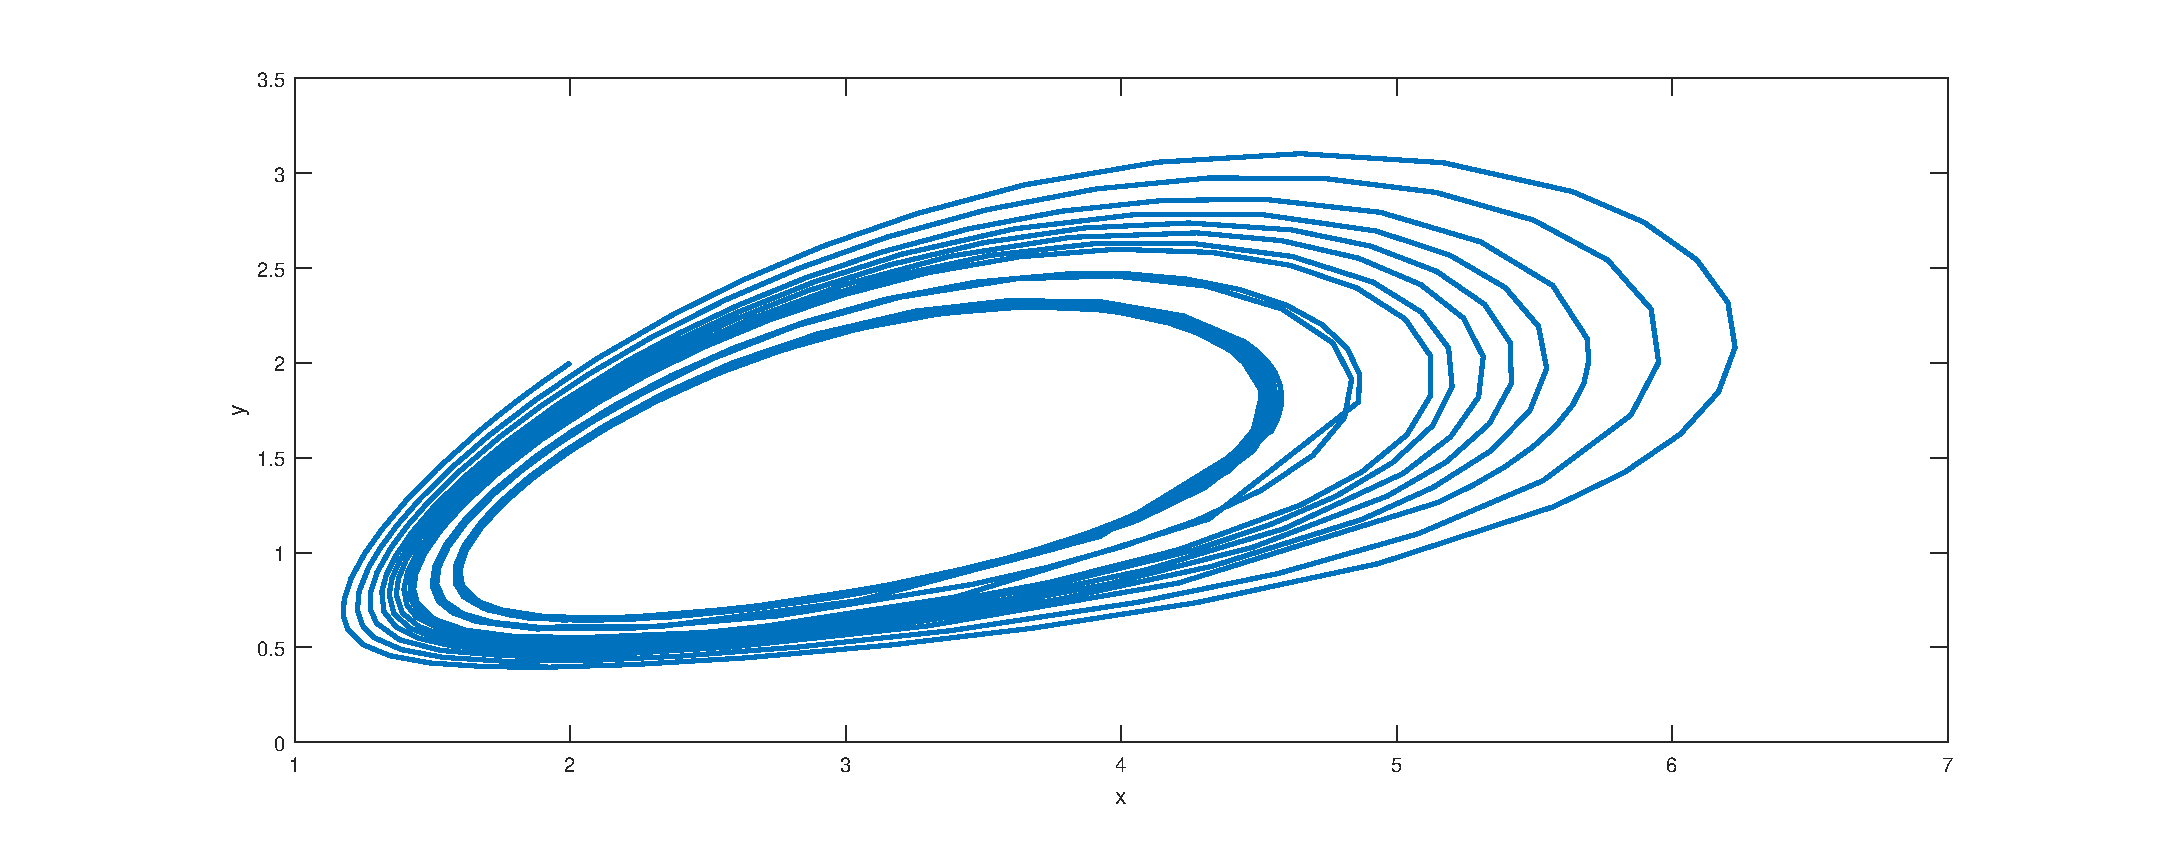
\includegraphics[width=9cm, height=6cm]{26b.eps}}
	\endminipage\hfill
	\begin{center} Figure 20: Time series of $x$ and $y$ (a) and phase portrait (b) for $\delta_0=0.7~\textless~\delta_0*.$ $E_*$ shows periodic solutions.  \end{center}
\end{figure}
From the figure, it is evident that $\delta_0~\textless~\delta_0^*,$ the system (3) is stable but as $\delta_0$ crosses its critical value($\delta_0^*=0.73$), the system exibits periodic solutions.

\begin{figure}[H]
	\minipage{0.5\textwidth}
	{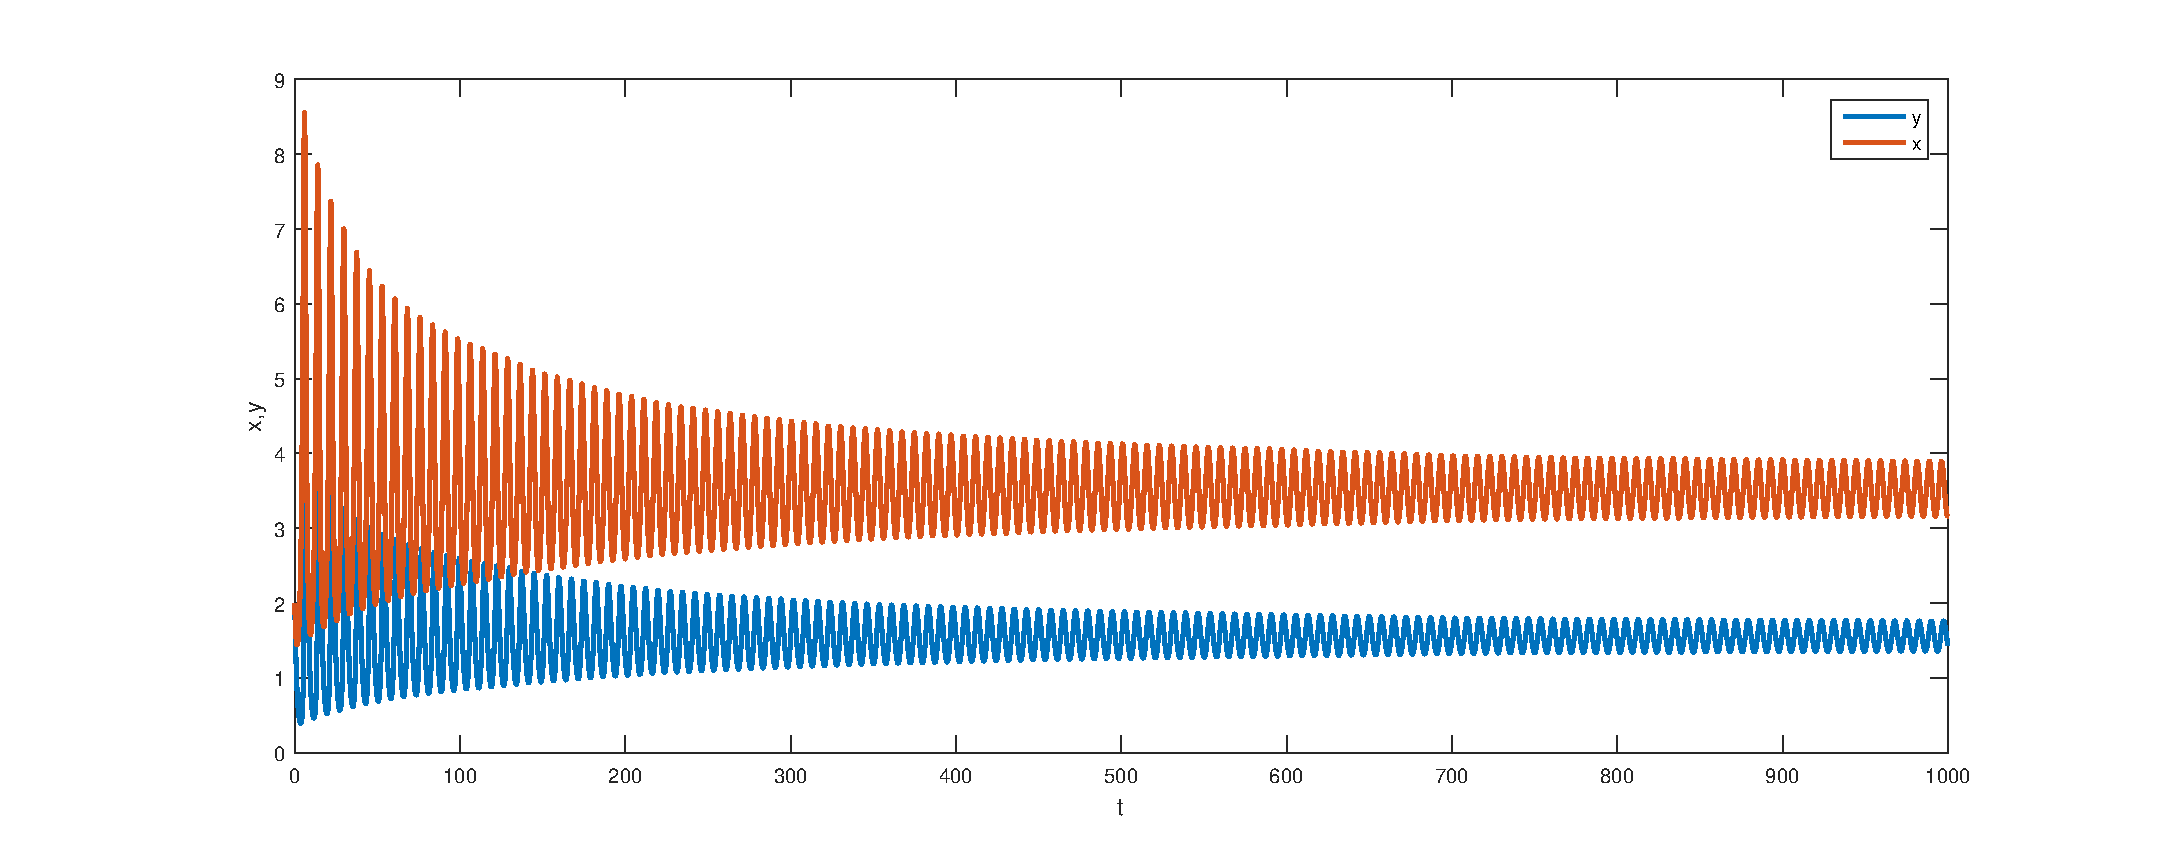
\includegraphics[width=9cm, height=6cm]{27a.eps}}
	\endminipage\hfill
	\minipage{0.5\textwidth}
	{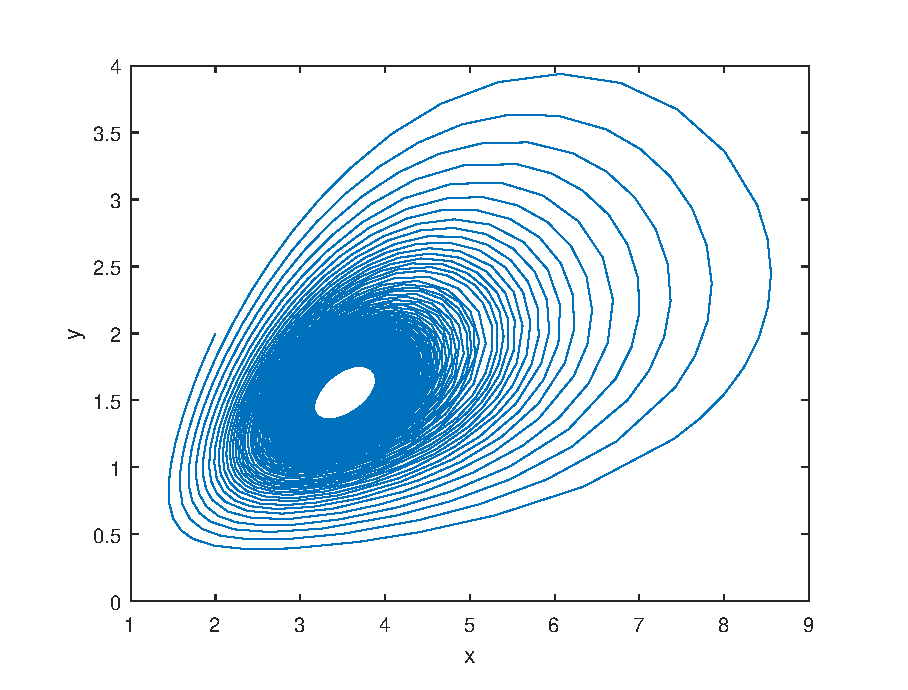
\includegraphics[width=9cm, height=6cm]{27b.eps}}
	\endminipage\hfill
	\begin{center} Figure 21: Time series of $x$ and $y$ (a) and phase portrait (b) for $\delta_1=0.2~\textless~\delta_1*.$ $E_*$ shows periodi solutions.  \end{center}
\end{figure}
From the figure, it is evident that $\delta_1~\textless~\delta_1^*,$ the system (3) is stable but as $\delta_1$ crosses its critical value($\delta_1^*=0.248$), the system exibits periodic solution.

\section{Conclusion} In this work, we made an attempt to discuss the impact of Allee effect (strong and weak both) in the model. They analyzed a density dependent non-linear mathematical model (1). In that model, prey grows logistically and predator fully depends on prey for food that followed by Beddington functional response.\par
Allee effect plays an important role in the structure of population. The Allee effect increases the possibilities of extinction. Thus, we include Allee effect into the model (1). Since there are two types of Allee effect; strong Allee effect and weak Allee effect so we studied both the models separately. In the study, we discussed positivity, boundedness of the solutions, existence of equilibrium points and their stability analysis of both the models. Positivity and boundedness of the solutions refer that the system is well behaved and not beyond to our nature.\par
We have shown that system (2) and (3) may have more than one interior equilibrium point. Under a sufficient condition (4) the systems have one interior equilibrium point. We also investigated a sufficient condition for asymptotic stability of interior equilibrium point. Then we found that model system (2) is bi-stable in the presence of positive equilibrium. The existence of periodic solution with respect to strong Allee parameter $\beta$ in model (2) and weak Allee parameter $\theta$ in model (3) also have been shown. We also observed that the time of fluctuations for both prey and predator increases with increment in Allee parameter for system (2). But after a critical value, interior equilibrium $E^*$ becomes unstable. In this situation system converges to stable trivial equilibrium $E_0,$ which shows extinction of species after a critical value of Allee parameter.\par

The numerical simulation is based on some hypothetical data to support our theoretical results. Time series and phase portrait diagram with respect to $\beta$ and $\theta$ help us to understand about the stability behavior of the system. This study is important to reduce the possibilities of extinction of species at low density level of prey population. We hope that our results in this work may help to understanding the dynamics of prey-predator system with Allee effect. \\\\



\textbf{\large References}\\
$[1]$Aziz-Alaoui MA, Okiye MD. Boundedness and global stability for a predator–prey model with modified Leslie–Gowerand Holling-type II schemes. Appl.Math.Lett 2003;16:1069–1075.\\
$[2]$OatenA, MurdochW. Functional response and stability in predator–prey systems. Am.Nat. 1975;109:289–298.\\
$[3]$Cantrell and Cosner,On the Dynamics of Predator–Prey Models with the Beddington–DeAngelis Functional Response. J.Math.Anal.Appl. 2001;257:206–222. \\
$[4]$Jian Zu, Masayasu Mimura, The impact of Allee effect on a predator–prey system with Holling type II functional response. Appl.Math.Comp. 2010;217:3542–3556.   \\
$[5]$Pallav Jyoti Pal, Prashanta Kumar Mandal, Bifurcation analysis of a modified Leslie–Gower predator–prey model with Beddington–DeAngelis functional response and strong Allee effect. Math.Comp.Simul. 2014;97:123-146 \\
$[6]$Haque M,A detailed study of the Beddington–DeAngelis predator–prey model.Math.Biosci. 2011;234:1–16.\\
$[7]$R.M. May, Stability and complexity in model ecosystems, Princeton University Press, 1973.\\
  

\end{document}